\documentclass[a4paper,justified,openany]{tufte-book}
\usepackage[utf8]{inputenc}
\usepackage[T1]{fontenc}

\usepackage{geometry}
\usepackage{soul}
\usepackage{amsmath}
\usepackage{ulem}
\usepackage{graphicx}
\graphicspath{{graphics/}}
\usepackage{upgreek}
\usepackage{amssymb}
\usepackage{esint}

\usepackage[caption=false]{subfig}
\usepackage[colorinlistoftodos]{todonotes}

\usepackage{hyperref}
\usepackage{color}
\usepackage{pdfpages}
\usepackage[version=3]{mhchem}

\usepackage{booktabs} % book-quality tables
\usepackage{multicol} % multiple column layout facilities
%\fvset{fontsize=\normalsize}% default font size for fancy-verbatim environments

% Formatting headers
\pagestyle{fancy}
\fancyhf{}
\rhead{Physique 3 - Ondes}
\lhead{\leftmark}
\cfoot{\thepage}

% Numbering chapters and sections
\setcounter{secnumdepth}{1}

\definecolor{bleuclair}{rgb}{0.7, 0.7, 1.0}
\usepackage[french]{babel}
% --------------------------------------------------------------------------------------------------------------------------------------------------------------------------------------------------------------------------------------------------------------------------

%%%%% REMARQUES GENERALES CONCERNANT CE FICHIER : 

%%%%%% Quand l'attention des professeurs est requise pour - un approfondissement - une vérification - (autre) : veuillez le signaler en commentaire avec, pour commencer :  /!\ PROFESSEURS 

%%%%%% Si vous désirez seulement ajouter des commentaires à ce qui a été écrit à un endroit : veuillez le signaler en commentaire avec, pour commencer : /!\ COMMENT 

%%%%%% Merci de votre compréhension et faisons de ce document un réel investissement collectif! 

% --------------------------------------------------------------------------------------------------------------------------------------------------------------------------------------------------------------------------------------------------------------------------

\begin{document}
	
	\title{Physique 3 - Ondes}
	\author{Martin Braquet\\Jérôme Louveaux\\Claude Oestges\\Balazs Udvarhelyi\\Guillaume Van Dessel}
	\publisher{École Polytechnique de Louvain}
	
	% Prints the month name (e.g., January) and the year (e.g., 2008)
	\newcommand{\monthyear}{%
		\ifcase\month\or January\or February\or March\or April\or May\or June\or
		July\or August\or September\or October\or November\or
		December\fi\space\number\year
	}
	
	
	% Prints an epigraph and speaker in sans serif, all-caps type.
	\newcommand{\openepigraph}[2]{%
		%\sffamily\fontsize{14}{16}\selectfont
		\begin{fullwidth}
			\sffamily\large
			\begin{doublespace}
				\noindent\allcaps{#1}\\% epigraph
				\noindent\allcaps{#2}% author
			\end{doublespace}
		\end{fullwidth}
	}
	
	\maketitle
	\vfill
	\openepigraph{
		Ce syllabus a été réalisé à l'issue du premier comité de  quadrimestre 2015 dans l'optique de créer un support de cours davantage formel et complet qui puisse aider les étudiants à approfondir leur compréhension de la matière. Il a été décidé qu' une collaboration étroite entre les étudiants et les professeurs du cours de Physique 3 soit établie afin de rendre ce document 
		le plus valable possible. \\
		Ce document est par conséquent modifiable par les étudiants et les professeurs; ces derniers vérifieront de temps à autre 
		son contenu et ajouteront des notes si nécessaire. \\
		Sous la supervision des professeurs, ce syllabus a été rédigé en majorité par trois étudiants: Martin Braquet (chapitres 5 et 6), Balazs Udvarhelyi (chapitres 4, 7 et l'annexe) et Guillaume Van Dessel (chapitres 1,2,3,4 et 8).
	}{ }
	\vfill
	\begin{figure*}
		\centering
		
\includegraphics[width=150pt]{epl.png}
	\end{figure*}
	\vfill
	
	\tableofcontents
	% AUTEUR :: Guillaume Van Dessel || SOURCE :: Slides || DATE :: 17.10.2015

\chapter{Champs électromagnétiques} 

 
\section{Introduction}

La première partie du cours de Physique 3 traite des champs électromagnétiques. \\
Comme son nom le suggère, le champ électromagnétique est un \textit{\textbf{champ vectoriel}} spatial
tri-dimensionnel (en toute généralité) dépendant également du \textit{temps}.  Il est la résultante d'une composante \textit{champ 
électrique} et d'une composante \textit{champ magnétique}. 

\section{Lois générales : formulation \textit{intégrale}}

Afin de se figurer comment une telle combinaison de champs se propage dans l'espace et le temps, il est nécessaire d'aborder les grandes 
lois de l'électricité et du magnétisme. 

\subsection{Rappels qualitatifs}
%\begin{fullwidth}



{\huge 1} : Des charges électriques \textit{\textbf{immobiles}} créent un \textit{\textbf{champ électrostatique}}.

\textit{Propriété} : Ce champ est \textit{conservatif} et dérive d'un \textbf{potentiel scalaire}.

\textit{Propriété} : \textbf{Force} sur charges électriques en mouvement et stationnaires.

{\huge 2} : Des courants constants\sidenote{Déplacements de charges électriques à débit constant} créent un \textit{\textbf{champ magnétique}} \sidenote{Champ magnétique \textit{d'excitation} $\vec{H}$ qui, couplé à la perméabilité magnétique de l'endroit où il vit donne le champ magnétique d'induction $\vec{B}$}\\constant.

\textit{Propriété} : Des charges en mouvement (accéléré ou non) créent des champs électriques se \textit{déplaçant}.

\textit{Propriété} : \textbf{Force} sur charges électriques en mouvement uniquement.

%\vspace{5mm} \hline \vspace{5mm}

\subsection{Théorème de Gauss dans la matière}

Le théorème de Gauss énonce que le flux du \textit{\textbf{champ de déplacement électrique}} ($\vec{D} = \epsilon_{r}\epsilon_{0}\vec{E} = \epsilon \vec{E}$)
à travers une surface \textit{fermée} vaut exactement la charge électrique comprise dans le volume qu'elle décrit dans l'espace. Cela se traduit par l'équation 

\begin{equation}
 \oint_{S} \vec{D} \cdot d\vec{s} = \int_{V} \rho dv = q_{incl}
 \label{GaussIntegral}
\end{equation}

\subsection{Absence de monopole magnétique}

Cette loi traduit le fait que le champ magnétique (d'\textit{excitation} ou \textit{induit}) n'admet pas de pôle. 
Autrement dit, chaque ligne de champ forme une \textit{courbe} fermée dans l'espace, de telle sorte que le flux 
du champ magnétique à travers une surface \textit{fermée} soit \textbf{nul}.

\begin{equation}
 \oint_{S} \vec{B} \cdot d\vec{s} = 0
 \label{MonoPoleIntegral}
\end{equation}

\subsection{Loi de Lenz-Faraday}

Comme le champ électrostatique dérive d'un potentiel scalaire, par définition mathématique, son intégrale le long 
d'une courbe \textit{fermée} dans l'espace est \textbf{nulle}. % /i\ COMMENT : L'intégrale dépend uniquement du point de départ à d'arrivée, le chemin emprunté n'importe pas. 
\textit{Cependant, si nous avons affaire à un flux magnétique dont la dérivée temporelle est non-nulle, le membre de droite de l'équation n'est plus nul !}

\begin{equation}
 \oint_{C} \vec{E} \cdot d\vec{l} = 0 \hspace{10pt} \mbox{ si } \frac{d\phi}{dt} \not = 0 \Rightarrow  \oint_{C} \vec{E} \cdot d\vec{l} = -\int_{S} \frac{\partial \vec{B}}{\partial t} \cdot d\vec{s}
 \label{PotentielIntegral}
\end{equation}

\subsection{Loi d'Ampère (incomplète)}

La Loi d'Ampère relie l'intégrale de contour du champ magnétique d'excitation au courant traversant la surface décrite par le contour en question. 
Comme nous allons le voir très bientôt, cette loi, formulée comme ci-dessous (équation \ref{AmpèreIntegral}), est \textbf{incomplète} car elle n'envisage pas toutes les géométries possibles.
\begin{equation}
 \oint_{C} \vec{H} \cdot d\vec{l} = I + ? = \int_{S} \vec{J} \cdot d\vec{s} + ? 
 \label{AmpèreIntegral}
\end{equation}

\section{Analyse vectorielle}

Nous avons découvert au quadrimestre passé les concepts de \textit{rotationnel}, \textit{divergence} pour un champ vectoriel et \textit{gradient} pour un champ scalaire.
Nous n'allons pas revenir sur ces concepts fondamentaux mais seulement rappeler deux définitions importantes qui nous permettront de construire les \textbf{lois de Maxwell}. 
Ces dernières sont réellement le ciment de notre connaissance concernant l'électricité et ses phénomènes.

\subsection{Divergence} 
\begin{marginfigure}[0cm]
	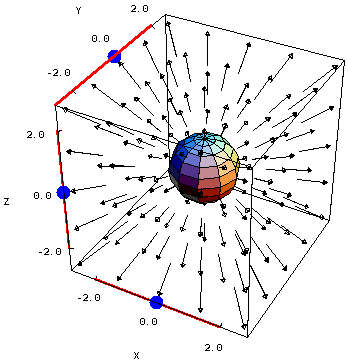
\includegraphics[width=4.5cm]{rep_div}
	\caption{Représentation de la divergence}
\end{marginfigure}

La divergence d'un champ vectoriel $\vec{F}$ satisfait les équations suivantes : 

\[ \text{div}(\vec{F}) = \nabla \cdot \vec{F} = \lim_{\Delta v \to 0} \frac{\oint_{S} \vec{F} \cdot d\vec{s}}{\Delta v} \]

\[\mbox{Théorème de la divergence : } \hspace{15pt} \oint_{S} \vec{F} \cdot d\vec{s} = \int_{V} (\nabla \cdot \vec{F}) \, dv\]

où $\Delta v$ correspond au volume \textit{infinitésimal} défini par la surface \textit{fermée} $S$.



\subsection{Rotationnel} 
\begin{marginfigure}
	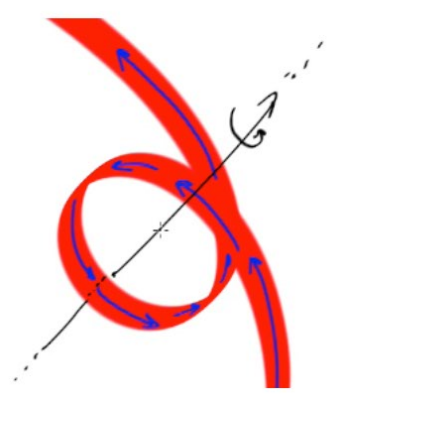
\includegraphics[width=4.5cm]{rep_rot}
	\caption{Représentation du rotationnel}
\end{marginfigure}

Le rotationnel\footnote{Le rotationnel est un concept inhérent à un espace tri-dimensionnel, nous pouvons le ramener à un espace de dimension moindre 
mais au delà de 3, il perd son sens.} d'un champ vectoriel $\vec{F}$ satisfait les équations suivantes  

\[  \vec{\text{rot}}(\vec{F}) \cdot \vec{n}   = (\nabla \times \vec{F}) \cdot \vec{n} = \lim_{\Delta s \to 0} \frac{\oint_{C} \vec{F} \cdot d\vec{l} }{\Delta s}\]

\[\mbox{Théorème de Stokes : } \hspace{15pt} \oint_{C} \vec{F} \cdot d\vec{l} = \int_{S} (\nabla \times \vec{F}) \cdot d\vec{s}\]

où $\Delta s$ correspond à la surface (aire) infinitésimale décrite par la courbe fermée $C$

\subsection{Propriétés des opérateurs différentiels}

Dans ce paragraphe, nous rappelons diverses propriétés des opérateurs différentiels que nous avons étudiées au second quadrimestre. 

\textit{Le rotationnel d'un champ vectoriel dérivant d'un potentiel scalaire est le champ «nul».} 

\[\nabla \times \nabla V = \vec{0} \] 

\textbf{NOTE :} Le rotationnel du champ électrostatique défini par $\vec{E} = -\nabla V$ est donc par conséquent nul !

\textit{La divergence d'un champ vectoriel rotationnel est  «nulle».}  

\[\nabla \cdot (\nabla \times \vec{A})  = 0 \]

\section{Equations de Maxwell}
Désormais, nous avons toutes les informations pour commencer à compléter les équations de Maxwell \sidenote{Enlever les intégrales revient à dire : \textit{\textbf{localement}}, l'équation est valable !}. 
Seule la Loi d'Ampère nécessitera une légère modification à la fin.

\begin{center}

\begin{tabular}{|c|c|}

\hline

1 & L'équation (1) devient : $ \oint_{S} \vec{D} \cdot d\vec{s}  =  \int_{V} (\nabla \cdot \vec{D} ) dv =  \int_{V} \rho dv$ \\  
- & $\Rightarrow \forall  \hspace{3pt} \mbox{ vol infinitésimal} \hspace{5pt} (\nabla \cdot \vec{D} ) = \rho$  \\

\hline

2 & L'équation (2) devient : $ \oint_{S} \vec{B} \cdot d\vec{s}  =  \int_{V} (\nabla \cdot \vec{B} ) dv =  \int_{V} 0 \:dv$ \\ 
- & $\Rightarrow \forall  \hspace{3pt} \mbox{ vol infinitésimal} \hspace{5pt} (\nabla \cdot \vec{B} ) = 0 $ \\

\hline

3 & L'équation (3) devient : $   \oint_{C} \vec{E} \cdot d\vec{l} = \int_{S} (\nabla \times \vec{E}) d\vec{s}= -\int_{S} \frac{\partial \vec{B}}{\partial t} \cdot d\vec{s}$ \\  
- &$ \Rightarrow \forall  \hspace{3pt} \mbox{ surf infinitésimale} \hspace{5pt} (\nabla \times \vec{E} ) = -\frac{\partial \vec{B}}{\partial t}$\\

\hline

\end{tabular}

\end{center}

\subsection{Terme manquant de la loi d'Ampère}

Nous allons ici montrer l'\textit{incohérence} de la loi d'Ampère pour certains cas de figure. \\
Prenons par exemple  le cas d'un circuit RC basique. Nous branchons en série une résistance $\mathcal{R}$ (ne joue pas de rôle particulier mais permet de formaliser les choses) et un condensateur plan $\mathcal{C}$ à une source de tension $\mathcal{V}$. Un courant $I_{c}(t)$ va naitre depuis la source de tension. Il passe à travers la résistance et atteint la borne \textbf{positive}\sidenote{Nous prenons la convention d'un courant de charges positives} du condensateur. Là, les particules sont théoriquement stoppées car le diélectrique présent entre les deux plaques assure une isolation électrique entre ces deux dernières.\sidenote{Jusqu'à une certaine tension de claquage évidemment} Il apparait alors une répulsion électrostatique de l'autre côté du condensateur plan  et un même nombre de particules, chargées positivement elles aussi, quitte la borne \textbf{négative} \sidenote{Négative car au fur et à mesure, une polarité négative s'installe étant donné que les particules chargées positivement quittent la paroi}. Si nous appliquons la loi d'Ampère sous forme intégrale en prenant en compte le vecteur densité de courant $\vec{J}$ et une surface définie par un cercle autour du conducteur électrique par lequel transite le courant total $I_{c}(t)$, nous avons alors 

\[  \oint_{C} \vec{H} \cdot d\vec{l} = I_{c}(t) = \int_{S} \vec{J} \cdot d\vec{s} \]

\begin{marginfigure}[0cm]
	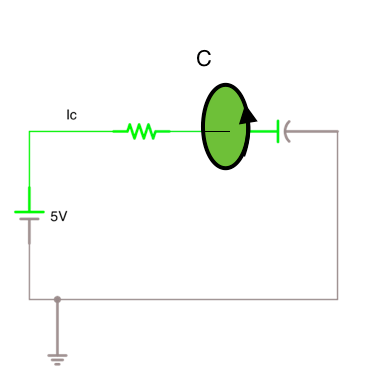
\includegraphics[width=5cm]{circ_ampere_naif}
	\caption{La surface plane définie par C intercepte le courant Ic}
\end{marginfigure}

Cependant, par la loi d'Ampère, nous pouvons prendre \textit{n'importe quelle surface définie par ce même cercle, le résultat devrait être \textbf{identique}}.

Tenons dès lors compte de ce même cercle avec le même circuit mais en changeant la surface considérée pour l'application de l'intégrale de surface de $\vec{J}$. 
Prenons désormais une demi-sphère de cercle principal le cercle autour du conducteur et englobant la borne \textbf{positive} du condensateur. La surface de cette demi-sphère sert
à l'intégration de $\vec{J}$. Nous avons : 

\[  \oint_{C} \vec{H} \cdot d\vec{l} =  \int_{S} \vec{J} \cdot d\vec{s} = I_{out}(t)\] 

où $I_{out}(t)$ représente le courant sortant de la borne \textbf{positive} du condensateur vers l'autre borne. 
\begin{marginfigure}[0cm]
	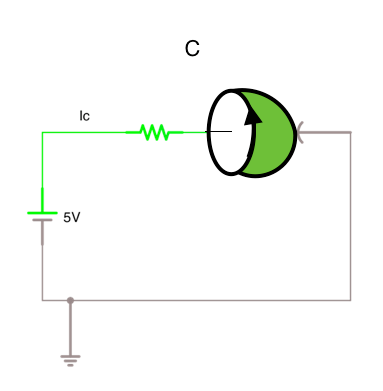
\includegraphics[width=5cm]{circ_ampere_bug}
	\caption{La surface de la semi-sphère définie par C n'intercepte pas le courant Ic}
\end{marginfigure}
Il est évidemment nul, par définition ! Dès lors, nous sommes confrontés à une contradiction : $I_{c}(t) = I_{out}(t) = 0\:?$ 

Cette contradiction peut être réglée par le développement suivant tiré des slides :
\[I_{c}(t) = \int_{S} \vec{J} \cdot d\vec{s} = -\frac{dQ_{out}(t)}{dt} = - \int \frac{d \sigma(t)}{dt} ds\] 
où $Q_{out}$ représente la charge de la borne \textbf{négative} du condensateur par où le courant $I_{c}(t)$ est «restitué».

Comme nous avons pour un condensateur plan les relations suivantes \sidenote{Certaines lettres représentent les normes de vecteurs qui leur sont associées. Ex : E = $\lvert\lvert\vec{E}\rvert\rvert$.}

\[ E \simeq \frac{V}{d} = \frac{Q}{Cd} = \frac{Qd}{\epsilon S d} = \frac{\sigma}{\epsilon} \Rightarrow \frac{\partial E}{\partial t} = \frac{1}{\epsilon} \frac{\partial \sigma}{\partial t} \]
où $d,V,Q,C,S,\sigma,E$ sont respectivement pour le condensateur la distance entre les deux plaques, la différence de potentiel électrique entre les deux plaques, la charge en valeur absolue de chacune des plaques, 
la capacité, la surface d'une des deux plaques, la densité de charge par plaque et le champ électrique entre les deux plaques.
Nous pouvons maintenant écrire :

\[ I_{c}(t) = \int_{S} \vec{J} \cdot d\vec{s} = -\int_{SurfOut} \epsilon \frac{\partial \vec{E}}{\partial t} \cdot d\vec{s} \]
\[ = - \int_{SurfOut} \frac{\partial \vec{D}}{\partial t} \cdot d\vec{s}  =  \int_{SurfOut} \vec{J}_{D} \cdot d\vec{s}\]
où $SurfOut$ représente la surface de la plaque associée à la borne \textbf{négative} du condensateur.

Entre les deux plaques du condensateur, nous pouvons donc observer une \textit{variation} du champ électrique au cours du temps. Cela implique en réalité une variation de champ magnétique par la même occasion ! \\
Posons alors que le terme manquant à notre loi d'Ampère soit $\frac{\partial \vec{D}}{\partial t}$. En effet, ce terme est en quelque sorte \textit{relié} à une variation de champ magnétique alors que le champ magnétique apparait dans l'intégrale du terme de gauche de la loi d'Ampère.
Nous aurions donc par la formule de Stokes : 

\[ \oint_{C} \vec{H} \cdot d\vec{l} = \int_{S} (\vec{J} +\frac{\partial \vec{D}}{\partial t}) \cdot d\vec{s} \]
\[ \Rightarrow \forall  \hspace{3pt} \mbox{surface infinitésimale,} \hspace{5pt} (\nabla \times \vec{H} ) = \vec{J} + \frac{\partial \vec{D}}{\partial t}\]

De plus, par la propriété des opérateurs différentiels qui dit que $\text{div}(\vec{\text{rot}}\:\vec{F}) = 0$, nous pouvons écrire : 

\[ \nabla \cdot (\vec{J} + \frac{\partial \vec{D}}{\partial t}) = 0 \Rightarrow \nabla \cdot \vec{J} = - \nabla \cdot \frac{\partial \vec{D}}{\partial t} = - \frac{\partial \rho}{\partial t}\]

Nous avons d'un côté de l'équation, un terme exprimant une \textit{somme de courants sortant en un endroit de l'espace} ($\nabla \cdot \vec{J}$) et de l'autre l'expression de l'\textit{évolution de la densité de charge en cet endroit} ($- \frac{\partial \rho}{\partial t}$). Le signe $-$ est tout à fait justifié. Une manière de s'en convaincre est la suivante : si nous avons des courants \textit{positifs}, alors la densité de charge diminuera mais le signe $-$ donnera un terme doublement négatif donc \textit{positif}.

\subsection{Expression générale du champ électrique}

Cette sous-section admet un objectif purement théorique. En effet, elle vise à exprimer, sur base de nos constats, le champ électrique de manière formelle. 
Repartons dès lors de la \textit{loi de Lenz-Faraday} écrite sous forme \textit{différentielle}.
Nous pouvons définir un \textit{\textbf{potentiel vecteur}} $\vec{A}$ tel que $\nabla \times \vec{A} = \vec{B}$\sidenote{Cette affirmation est vraie pour tout champ vectoriel $\vec{B}$ \textit{régulier} et de \textit{divergence nulle} sur un domaine \textit{ouvert et étoilé}.}. Dès lors, nous pouvons écrire 

\[\nabla \times \vec{E} = - \frac{\partial \vec{B}}{\partial t} = -\frac{\partial (\nabla \times \vec{A})}{\partial t} = - \nabla \times \frac{\partial \vec{A}}{\partial t} \]
\[\nabla \times (\vec{E} + \frac{\partial \vec{A}}{\partial t}) = \vec{0} \]

Ce qui veut dire, par la propriété différentielle $\vec{\text{rot}}(\text{grad}\:V) = \vec{0}$ que $(\vec{E} + \frac{\partial \vec{A}}{\partial t})$ dérive d'un potentiel scalaire.
Nous supposons qu'il s'agit bien du potentiel électrique $\mathcal{V}$. Nous spécifions alors l'équation finale exprimant $\vec{E}$ : 

\[(\vec{E} + \frac{\partial \vec{A}}{\partial t}) = - \nabla \mathcal{V} \Rightarrow \vec{E} = - (\nabla \mathcal{V} + \frac{\partial \vec{A}}{\partial t}) \]
 
 \subsection{Conditions aux interfaces}
 
 Les lois de Maxwell gouvernent aussi la continuité des champs électromagnétiques aux interfaces entre deux milieux aux propriétés électromagnétiques différentes.
 
 \begin{marginfigure}[-10cm]\\
 	\normalsize 
 	\label{interface1}
 	\caption{\textit{\textbf{En absence de charges et de courants de surface}} à l'interface: }
	\begin{center}
	\begin{tabular}{|ccc|}
		\hline
		$\vec{D}_{1,n} $ & = & $\vec{D}_{2,n} $ \\
		$\vec{B}_{1,n} $ & = & $\vec{B}_{2,n} $ \\
		$\vec{E}_{1,t} $ & = & $\vec{E}_{2,t} $ \\
		$\vec{H}_{1,t} $ & = & $\vec{H}_{2,t} $ \\
		\hline
	\end{tabular}
	
	%%%%% /!\ PROFESSEURS : Puisque D et E et B et H sont, dans notre théorie, égaux à une constante de proportionnalité près. Pourquoi dans le cas du déplacement électrique et de 
	%%%%% l'induction magnétique impose t'on la continuité de la composante normale à l'interface alors qu'avec le champ électrique et l'excitation magnétique ce sont les composantes tangentielles qui
	%%%%% requièrent la continuité ? Merci d'avance.  
	
	%%%%% /!\ COMMENT : vidéo trouvée expliquant le phénomène : https://www.youtube.com/watch?v=wahmW7h-AKo&feature=youtu.be&t=10m21s
	
	%\includegraphics[height = 130pt, width = 400pt]{milieux.png} 
	
	\end{center}

 \end{marginfigure}
 
  \begin{marginfigure}[-2cm]
 	\normalsize 
 	\caption{Les conditions aux limites deviennent alors (en toute généralité):}
 	\begin{center}
 		\begin{tabular}{|ccc|}
 			\hline
 			$\vec{n} \cdot (\vec{D}_{1} - \vec{D}_{2}) $ & = & $ \rho_S$ \\
 			$\vec{n} \cdot (\vec{B}_{1} - \vec{B}_{2}) $ & = & $ 0 $ \\
 			$\vec{n} \times (\vec{E}_{1} - \vec{E}_{2}) $ & = & $ 0$ \\
 			$\vec{n} \times (\vec{H}_{1} - \vec{H}_{2}) $ & = & $ \vec{K}$ \\
 			\hline
 		\end{tabular}
 	\end{center}
 	
 	En l'absence de charges et courants de surface, $\rho_S = 0$ et $\vec{K} = \vec{0}.$
 	
 	% \textbf{NOTE : } Il y a deux directions $\hat{t}$ car en réalité quand nous %parlons de direction tangentielle à l'interface (Ex : $\vec{H}_{1,t}$), 
 	%nous voulons plutôt signifier: pour la partie tangentielle à l'interface, la %condition de continuité s'applique. Mais comme à la surface de l'interface il %existe un plan entier admettant 
 	%des directions tangentielles, nous devons donc rajouter une deuxième %dimension avec le second vecteur unitaire $\hat{t}$ pointant vers le lecteur.
 \end{marginfigure}
 
 Pour démontrer le résultat de la figure \ref{interface1}, partons des équations de Maxwell. On imagine au niveau de l'interface un petit cylindre de section $dS$ (dont l'axe est perpendiculaire à l'interface) et une boucle de longueur $dl$ (dont l'axe est parallèle à l'interface). 
\begin{itemize}
\item Si le champ électrique est purement normal, la loi de Gauss appliquée au cylindre  implique que $\vec{D}_{1}\cdot d\vec{S_1} +  \vec{D}_{2}\cdot d\vec{S_2} = Q_{int} = \rho_S dS$; comme $d\vec{S_1} = \vec{n}dS = -d\vec{S_2}$, on trouve que $\vec{n}\cdot(\vec{D}_{1} - \vec{D}_{2}) = \rho_S$. En l'absence de charges à l'interface, $\rho_S = 0$ et donc, $\vec{n}\cdot(\vec{D}_{1} - \vec{D}_{2}) = 0$, soit ${D}_{1,n} = {D}_{2,n}$.
\item Sur base de la loi sur le flux du magnétique, on trouve de manière similaire pour un champ magnétique purement normal que $\vec{n}\cdot(\vec{B}_{1} - \vec{B}_{2}) = 0$, soit ${B}_{1,n} = {B}_{2,n}$.
\item Si le champ électrique est purement tangentiel, la loi de circulation de $\vec{E}$ sur la boucle donne $\vec{E}_1\cdot d\vec{l_1} + \vec{E}_2\cdot d\vec{l_2} = 0$; comme $d\vec{l_1} = - d\vec{l_2}$, on trouve  ${E}_{1,t} =  {E}_{2,t}$.
\item Si le champ magnétique est purement tangentiel, l'application de la loi d'Ampère sur la boucle donne $\vec{H}_1\cdot d\vec{l_1} + \vec{H}_2\cdot d\vec{l_2} = I_{enc}$. Si un courant de surface $\vec{K}$ existe, alors $I_{enc} = \vec{K} d\cdot{l_1}$, puisqu'un courant de surface est défini en Ampères par mètre de largeur. En l'absence de courant à la surface, on trouve que ${H}_{1,t} =  {H}_{2,t}$.
\end{itemize} 
 
% \includegraphics[height = 150pt, width = 250pt]{interface.png} 
Ces lois sont également valables si les champs ne sont pas purement normaux ou tangentiels : il suffit de prendre la projection normale ou tangentielle des champs.\sidenote[][-8cm]{Il y a une infinité de directions tangentielles à l'interface: dès lors, on ne spécifie pas de vecteur tangentiel comme on le fait pour le vecteur normal, noté $\vec{n}$ et pris par convention comme pointant du milieu 2 vers le milieu 1; quand on parle de direction tangentielle à l'interface (Ex : $\vec{H}_{1,t}$), 
	on veut bien signifier la projection sur l'interface du champ vectoriel: pour la partie tangentielle à l'interface, la condition de continuité s'applique. Une manière élégante de représenter cette projection est d'écrire, par exemple, ${H}_{1,t}\vec{t} = \vec{n} \times \vec{H}_{1}$. }
% /!\ COMMENT & /!\ PROFESSEURS
  %  Quid de cette phrase ? :) (voir en dessous) 
 %Les champs ne sont donc pas, en toute généralité, continus à une interface ! \\ \\
 

 %\todo{Expliquer illustration divergeance et rotationnel.}
 %\subsection{Résumé (slide)}
 %\includegraphics[height = 300pt, width = 450pt]{CM1.png}

	\chapter{Ondes électromagnétiques}

%%%%% /!\ PROFESSEURS : Quid des singularités pour l'espace? Nous parlons d'un espace vide de charges et de courants en ce qui concerne les ondes EM mais pourquoi ? 
%%%%% Comment se figurer un tel espace? Aussi, il semble que les ondes EM se propagent très bien malgré la présence de charges ou de courants?  ==>> CLARIFICATION NECESSAIRE

Dans cette section, nous allons aborder une partie primordiale du cours qui concerne les ondes électromagnétiques. \\
\textit{Qu'est ce qu'une onde électromagnétique}? Nous pouvons définir une onde EM comme la \textbf{propagation d'un signal} à travers l'espace; 
ce signal correspond à une \textbf{\textit{variation couplée}} d'un champ électrique et d'un champ magnétique.  Ce signal se transmet à une vitesse qui est propre au milieu traversé comme nous le verrons à la section suivante. 
Pour l'instant, nous allons partir des équations de Maxwell pour aboutir sur l'équation définissant les ondes EM. Pour rester relativement global tout en simplifiant parfois les choses, nous approcherons le problème de manière générale et traiterons ensuite en profondeur des cas particuliers. 
\footnote{Théorie provenant conjointement des slides et de \textit{wikipédia} : \url{https://fr.wikipedia.org/wiki/Établissement_de_l\%27équation_de_propagation_à_partir_des_équations_de_Maxwell}}

%\subsection{Formulation générale et équation d'Alembert}

\section{Notions et notations}

Cette sous-section vise à introduire les notions mathématiques et physiques dont nous aurons besoin afin d'arriver à nos fins. 
%\begin{fullwidth}
%	\begin{center}
%		
%		\begin{tabular}{|c|c|c|}
%			
%			\hline
%			
%			1 & Champ électrique & $\vec{E}(x,y,z,t) = E_{x}(x,y,z,t) \hat{x} + E_{y}(x,y,z,t) \hat{y} + E_{z}(x,y,z,t) \hat{z}$ \\
%			
%			\hline
%			
%			2 & Champ magnétique d'excitation &  $\vec{H}(x,y,z,t) = H_{x}(x,y,z,t) \hat{x} + H_{y}(x,y,z,t) \hat{y} + H_{z}(x,y,z,t) \hat{z}$ \\
%			
%			\hline 
%			
%			3 & \textit{\textbf{Laplacien}} vectoriel & $\Delta \vec{R} = \nabla^{2}(R_{x}(x,y,z,t) \hat{x} + R_{y}(x,y,z,t) \hat{y} + R_{z}(x,y,z,t) \hat{z}) $\\
%			
%			\hline
%			
%			4 & Propriété & $\nabla \times (\nabla \times \vec{R}) = \nabla(\nabla \cdot \vec{R}) - \Delta \vec{R} $\\
%			
%			\hline
%			
%			5 & Première équation de \textit{\textbf{Maxwell}} & $\nabla \cdot \vec{E} = \frac{\rho}{\epsilon}$ \\
%			
%			
%			6 & Troisième équation de \textit{\textbf{Maxwell}} & $\nabla \times \vec{E} = - \mu \frac{\partial \vec{H}}{\partial t}$ \\
%			
%			
%			7 & Quatrième équation de \textit{\textbf{Maxwell}} & $\nabla \times \vec{H} =  \vec{J} + \epsilon \frac{\partial \vec{E}}{\partial t}$ \\
%			
%			\hline
%			
%		\end{tabular}
%		
%	\end{center}
%\end{fullwidth}
\begin{enumerate}
\item{Champ électrique} \begin{center}$\vec{E}(x,y,z,t) = E_{x}(x,y,z,t) \hat{x} + E_{y}(x,y,z,t) \hat{y} + E_{z}(x,y,z,t) \hat{z}$\end{center} 
\item{Champ magnétique d'excitation } \begin{center}$\vec{H}(x,y,z,t) = H_{x}(x,y,z,t) \hat{x} + H_{y}(x,y,z,t) \hat{y} + H_{z}(x,y,z,t) \hat{z}$\end{center} 
\item{\textit{\textbf{Laplacien}} vectoriel} \begin{center} $\Delta \vec{R} = \nabla^{2}(R_{x}(x,y,z,t) \hat{x} + R_{y}(x,y,z,t) \hat{y} + R_{z}(x,y,z,t) \hat{z}) $\end{center} 
\item{Propriété} 
\begin{center}$\nabla \times (\nabla \times \vec{R}) = \nabla(\nabla \cdot \vec{R}) - \Delta \vec{R} $\end{center} 
\item{Première équation de \textit{\textbf{Maxwell}}} 
\begin{center}$\nabla \cdot \vec{E} = \frac{\rho}{\epsilon}$\end{center} 
\item{Troisième équation de \textit{\textbf{Maxwell}}}
\begin{center}
$\nabla \times \vec{E} = - \mu \frac{\partial \vec{H}}{\partial t}$
\end{center} 
\item{Quatrième équation de \textit{\textbf{Maxwell}}} \begin{center} $\nabla \times \vec{H} =  \vec{J} + \epsilon \frac{\partial \vec{E}}{\partial t}$\end{center} 
\end{enumerate}
\section{Développement par combinaison}

Maintenant que nous avons introduit les différentes données de notre développement, nous pouvons  commencer à combiner les équations. 
Si nous dérivons la quatrième équation de Maxwell (7) par rapport au temps, nous pouvons écrire\sidenote{Grâce au théorème de \textbf{Schwarz}.} 

\[ \frac{\partial (\nabla \times \vec{H})}{\partial t} = \nabla \times \frac{\partial \vec{H}}{\partial t} = \frac{\partial(\vec{J} + \epsilon \frac{\partial \vec{E}}{\partial t})}{\partial t} \]

Nous nous rendons rapidement compte que cette dérivée partielle peut également faire apparaitre la troisième équation de Maxwell : 

\[ \nabla \times \frac{\partial \vec{H}}{\partial t} = -\frac{1}{\mu}( \nabla \times (\nabla \times \vec{E}))\]

En recombinant rapidement ces deux équations, nous pouvons mettre en exergue la relation suivante : 

\[-\mu(\frac{\partial \vec{J}}{\partial t} + \epsilon \frac{\partial^{2} \vec{E}}{\partial t^{2}}) = \nabla \times (\nabla \times \vec{E})\]

Etant donnée la propriété\sidenote{Que nous n'allons pas démontrer car cette démonstration sort du cadre du cours.} (4 ème entrée du tableau) concernant le rotationnel du rotationnel, 
nous pouvons écrire la dernière équation sous une forme ne faisant plus intervenir le rotationnel : 

\[ \Delta \vec{E} - \mu \epsilon  \frac{\partial^{2} \vec{E}}{\partial t^{2}} = \mu \frac{\partial \vec{J}}{\partial t} + \nabla(\nabla \cdot \vec{E}) \]

La première équation de Maxwell nous permet d'affiner notre équation d'onde en jouant avec les densités de charge : 

\[ \Delta \vec{E} - \mu \epsilon  \frac{\partial^{2} \vec{E}}{\partial t^{2}} = \mu \frac{\partial \vec{J}}{\partial t} + \frac{\nabla \rho}{\epsilon} \]

\section{Cas particulier des conducteurs ohmiques}

Pour les \textit{conducteurs Ohmiques}, la loi d'\textit{Ohm} lie le vecteur densité de courant au champ électrique. \\
Cette dernière s'écrit de la manière suivante : 

\[\vec{J} = \sigma_{\Omega} \vec{E} \]

où $\sigma_{\Omega}$ représente la \textit{conductivité électrique}.\footnote{L'inverse de la \textit{résistivité}.} En introduisant ceci dans la dernière équation et en considérant que la
\textit{densité de charge} reste \textit{constante} 

\[ \Delta \vec{E} - \mu \epsilon  \frac{\partial^{2} \vec{E}}{\partial t^{2}} = \mu \sigma_{\Omega} \frac{\partial \vec{E}}{\partial t} \]
Nous allons voir plus loin ce que cela représente vraiment mais voici l'\textit{impédance caractéristique} du système en $\vec{E},\vec{H}$ : 

\[ \frac{|| \vec{E} ||}{|| \vec{H} ||} =  \frac{E}{H} =\sqrt{\frac{\mu}{\sqrt{\epsilon(1+\frac{\sigma_{\Omega}^{2}}{\epsilon^{2} \omega^{2}})}}}\]

\section{Cas particulier du vide (3D)} 

Dans le \textit{cas particulier du \textbf{vide}}, nous avons affaire à une \textit{densité de charge} supposée \textit{constante} ainsi que des \textit{densités de courant} supposées \textit{nulles} également.
($\epsilon = \epsilon_{0}$ et $\mu = \mu_{0}$)

\[ \Delta \vec{E} = \mu \epsilon  \frac{\partial^{2} \vec{E}}{\partial t^{2}} = \mu_{0} \epsilon_{0}  \frac{\partial^{2} \vec{E}}{\partial t^{2}} =\frac{1}{c^{2}} \frac{\partial^{2} \vec{E}}{\partial t^{2}} \]

où $c^{2}$ est la \textit{vitesse de la lumière} au carré ($c = 299 792 458 [m/s]$).

\begin{center}
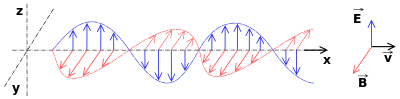
\includegraphics[height = 100pt, width = 300pt]{ondeEM.png}
\end{center}


\section{Cas particulier du vide (1D) : équations d'Alembert}

Nous allons traiter ici du \textit{cas particulier du \textbf{vide}} en une seule dimension spatiale.  \\
C'est à dire que nous allons considérer que le champ électrique ne dépend que d'une seule variable spatiale et du temps et pointe dans une seule direction (qui n'est pas celle de la variable pour éviter la confusion par après).
Nous écrivons alors $\vec{E}(x,y,z,t) \Rightarrow \vec{E_{y}}(x,t)$. \\
Il en est de même pour le champ magnétique d'excitation (ou d'induction) nous considérons qu'il est 
\textit{orthogonal} au champ électrique et dépend aussi de $x$ et $t$ seulement ; $\vec{H}(x,y,z,t) \Rightarrow \vec{H_{z}}(x,t)$. 

\begin{itemize}
	\item
Soit nous repartons de ce que nous avons déjà fait pour le cas général, l'équation d'onde est alors immédiate. \\
En effet, en 1D, le \textbf{Laplacien} vectoriel de $\vec{E}$ donne simplement sa dérivée partielle seconde en son unique variable
spatiale : 
\[ \Delta \vec{E} = \mu_{0} \epsilon_{0}  \frac{\partial^{2} \vec{E}}{\partial t^{2}} \Rightarrow \frac{\partial^{2} \vec{E} }{\partial x^2} = \frac{1}{c^{2}}  \frac{\partial^{2} \vec{E}}{\partial t^{2}}\]
qui se résout de manière \textit{scalaire} pour la direction unitaire de la variable ($y$ par exemple ici) : 
\[\frac{\partial^{2} E_{y}}{\partial x^{2}} = \frac{1}{c^{2}}  \frac{\partial^{2} E_{y}}{\partial t^{2}}\]


\item Soit nous repartons de zéro et adoptons une méthode plus \textit{faible} mathématiquement parlant et faisons les hypothèses suivantes.\\
Nous admettrons pour ce qui suit que la matrice \textit{Hessienne} des uniques fonctions scalaires liées à $\vec{E}$ et $\vec{H}$ soit symétrique. 
Plus particulièrement, nous pouvons imposer que ces fonctions soient de classe $\mathcal{C}^{2}$ ce qui vérifie la condition sur la \textit{Hessienne}.

Nous pouvons dès lors écrire, tout en se basant sur les équations de Maxwell : 


\begin{equation*}
	\begin{split}
\nabla \times \vec{E} =& -\mu_{0} \frac{\partial \vec{H}}{\partial t} \\=& (\frac{\partial E_{z}}{\partial y} - \frac{\partial E_{y}}{\partial z})\hat{x} +   (\frac{\partial E_{x}}{\partial z} - \frac{\partial E_{z}}{\partial x})\hat{y} +
(\frac{\partial E_{y}}{\partial x} - \frac{\partial E_{x}}{\partial y})\hat{z} \\=& \frac{\partial E_{y}}{\partial x} \hat{z}
	\end{split}
\end{equation*}
\begin{equation*}
\begin{split}
\nabla \times \vec{H} &= \epsilon_{0} \frac{\partial \vec{E}}{\partial t} \\&= (\frac{\partial H_{z}}{\partial y} - \frac{\partial H_{y}}{\partial z})\hat{x} +   (\frac{\partial H_{x}}{\partial z} - \frac{\partial H_{z}}{\partial x})\hat{y} +
(\frac{\partial H_{y}}{\partial x} - \frac{\partial H_{x}}{\partial y})\hat{z} \\&= -\frac{\partial H_{z}}{\partial x} \hat{y}
	\end{split}
\end{equation*}

Nous possédons alors un système d'EDP linéaires couplées deux à deux de premier ordre. \\
La résolution de ce genre de système est un problème typique lié aux \textit{équations aux dérivées partielles} et est abordé dans le cours
de mathématiques 3. Nous allons ici transformer ce système en deux EDP linéaires de second ordre dont la résolution est semblable. \\
Nous pouvons dériver la première équation ci-dessus par rapport à $x$ et la seconde par rapport au temps $t$ : 

\[  \frac{\partial^{2} \vec{H}}{\partial x \partial t} = -\frac{1}{\mu_{0}} \frac{\partial^{2} E_{y}}{\partial x^{2}} \hat{z}\]
\[  \frac{\partial^{2} H_{z}}{\partial t \partial x} \hat{y} = - \epsilon_{0} \frac{\partial^{2} \vec{E}}{\partial t^{2}} \]

Comme les dérivées partielles secondes sont \textit{croisées} et si nous travaillons en termes de \textbf{\textit{normes}} :

\[\frac{\partial^{2} E_{y}}{\partial x^{2}} = \frac{1}{c^{2}}  \frac{\partial^{2} E_{y}}{\partial t^{2}} \hspace{10pt} \mbox{||} \hspace{10pt} \frac{\partial^{2} H_{z}}{\partial x^{2}} = \frac{1}{c^{2}}  \frac{\partial^{2} H_{z}}{\partial t^{2}}\]
\end{itemize}

\textit{Les EPD de second ordre linéaires homogènes en 1D (et temps) de type hyperbolique} admettent une solution générale du type\footnote{A nouveau, se référer au cours de Mathématiques 3}  : 
$ \xi(x,t) = \frac{1}{2}(f(x-ct)+f(x+ct)) $. \\ 
Dans le cas d'ondes, nous travaillerons souvent avec des fonctions $f$ sinusoïdales admettant parfois un déphasage $\phi$ çà et là. 
 

\section{Propriétés des EDP linéaires couplées de premier ordre (1D et temps)}

De manière tout à fait générale, si deux grandeurs \textit{scalaires} A et B dépendant d'une variable temporelle et une variable spatiale sont 
liées par des équations de type 

\[\frac{\partial A}{\partial x} = -\alpha \frac{\partial B}{\partial t}\]

\[\frac{\partial A}{\partial t} = -\beta \frac{\partial B}{\partial x}\]

elles \textbf{obéissent toutes deux à une même équation d'onde de type} : $\frac{1}{c^{2}} \frac{\partial^{2} A,B}{\partial t^{2}} = \frac{\partial^{2} A,B}{\partial x^{2}}$. 
Le paramètre $c$ représente toujours la \textit{vitesse} de propagation de la grandeur scalaire et vaut : $c = \sqrt{\frac{\beta}{\alpha}}$. 
Le rapport entre ces deux grandeurs est nommé \textit{impédance caractéristique} et vaut quant à elle : $\mathcal{Z} = \sqrt{\alpha\beta}$.\footnote{Les grands voyageurs parmi vous auront immédiatement reconnu la fameuse enseigne grecque :\\ le supermarché low-cost Alpha-Beta} 

Nous pouvons prouver l'existence d'un tel $\mathcal{Z}$ comme marqué dans les slides. Soient donc deux solutions à l'équation d'onde et aux équations couplées données par les expressions suivantes :

\[S_{1}(x,t) = \mathcal{F}(x-ct) + \mathcal{F}(x+ct)\]
\[S_{2}(x,t) = \mathcal{G}(x-ct) + \mathcal{G}(x+ct)\]

Si nous posons $w = x-ct$ et $u = x+ct$ nous pouvons écrire grâce aux équations couplées : 
\begin{fullwidth}
	\[\frac{\partial S_{1}}{\partial x} = -\alpha \frac{\partial S_{2}}{\partial t} \Leftrightarrow \frac{\partial \mathcal{F}(w)}{\partial w}\frac{\partial w}{\partial x} + \frac{\partial \mathcal{F}(u)}{\partial u}\frac{\partial u}{\partial x} 
	= -\alpha (\frac{\partial \mathcal{G}(w)}{\partial w}\frac{\partial w}{\partial t} + \frac{\partial \mathcal{G}(u)}{\partial u}\frac{\partial u}{\partial t})\]
	
	\[\frac{\partial S_{1}}{\partial t} = -\beta \frac{\partial S_{2}}{\partial x} \Leftrightarrow \frac{\partial \mathcal{F}(w)}{\partial w}\frac{\partial w}{\partial t} + \frac{\partial \mathcal{F}(u)}{\partial u}\frac{\partial u}{\partial t} 
	= -\beta (\frac{\partial \mathcal{G}(w)}{\partial w}\frac{\partial w}{\partial x} + \frac{\partial \mathcal{G}(u)}{\partial u}\frac{\partial u}{\partial x})\]
\end{fullwidth}	
	En simplifiant les équations : 
\begin{fullwidth}	
	\begin{equation}
	\frac{\partial \mathcal{F}(w)}{\partial w} + \frac{\partial \mathcal{F}(u)}{\partial u}
	= -\alpha (-c \frac{\partial \mathcal{G}(w)}{\partial w} + c \frac{\partial \mathcal{G}(u)}{\partial u}) \Rightarrow
	\frac{\partial \mathcal{F}(w)}{\partial w} + \frac{\partial \mathcal{F}(u)}{\partial u} = -\alpha c (-\frac{\partial \mathcal{G}(w)}{\partial w} +\frac{\partial \mathcal{G}(u)}{\partial u}) 
	\end{equation}
	
	\begin{equation}
	-c \frac{\partial \mathcal{F}(w)}{\partial w} + c \frac{\partial \mathcal{F}(u)}{\partial u}
	= -\beta (\frac{\partial \mathcal{G}(w)}{\partial w} + \frac{\partial \mathcal{G}(u)}{\partial u}) \Rightarrow -\frac{\partial \mathcal{F}(w)}{\partial w} + \frac{\partial \mathcal{F}(u)}{\partial u}
	= -\frac{\beta}{c} (\frac{\partial \mathcal{G}(w)}{\partial w} + \frac{\partial \mathcal{G}(u)}{\partial u})
	\end{equation}
\end{fullwidth}	

En additionnant les équations (5) et (6), et en définissant $\mathcal{Z} = \frac{\beta}{c} = \alpha c$ nous obtenons : 

\begin{equation}
 \frac{\partial \mathcal{F}(u)}{\partial u} =  \mathcal{Z} \frac{\mathcal{G}(u)}{\partial u}
\end{equation}

Ce qui donne, après intégration (le résultat est exactement symétrique pour le cas $\mathcal{F}(w), \mathcal{G}(w)$) 

\[\mathcal{F}(u) = \mathcal{Z} \cdot \mathcal{G}(u) + \mathcal{K}\]

Si nous considérons des \textbf{phénomènes physiques} de \textit{propagation}, la constante $\mathcal{K}$ est tout simplement nulle car 
à l'origine, la propagation n'a pas encore eu lieu. 


Etant donnée la symétrie des équations, nous pouvons tirer la même conclusion quant aux grandeurs $\mathcal{S}_{1},\mathcal{S}_{2}$. 
Immédiatement, il vient que l'\textit{impédance caractéristique} d'une onde\\ électromagnétique, en considérant le vecteur $\vec{J}$ nul, vaut 
$\mathcal{Z} = \sqrt{\frac{\mu}{\epsilon}} \simeq120 \pi \simeq 377 [\Omega] $. 

\section{Représentation du cas particulier 1D}

Etant donné que nous avons pu caractériser l'équation d'onde du cas particulier et en tirer certaines conclusions, 
voici donc la forme générale du champ électrique d'une \textit{onde EM plane monochromatique} (\textit{polarisée linéairement}, nous y reviendrons).

\[\vec{E}(x,y,z,t) \Rightarrow \vec{E}_{y}(x,t) = \xi sin(k x - \omega t + \phi) \hat{y} \]
où $\xi,\omega,t,k,x,\phi$ sont respectivement l'élongation maximale en chaque point de l'espace, la \textit{pulsation} (la fréquence  vaut $f = \frac{w}{2 \pi} = \frac{1}{T}$ où $T$ 
est la période du signal), le temps, le nombre d'onde ($k = \frac{2\pi}{\lambda}$ où $\lambda$ est la longueur d'onde), la position sur l'axe des X, le déphasage  du champ électrique. 
\begin{marginfigure}
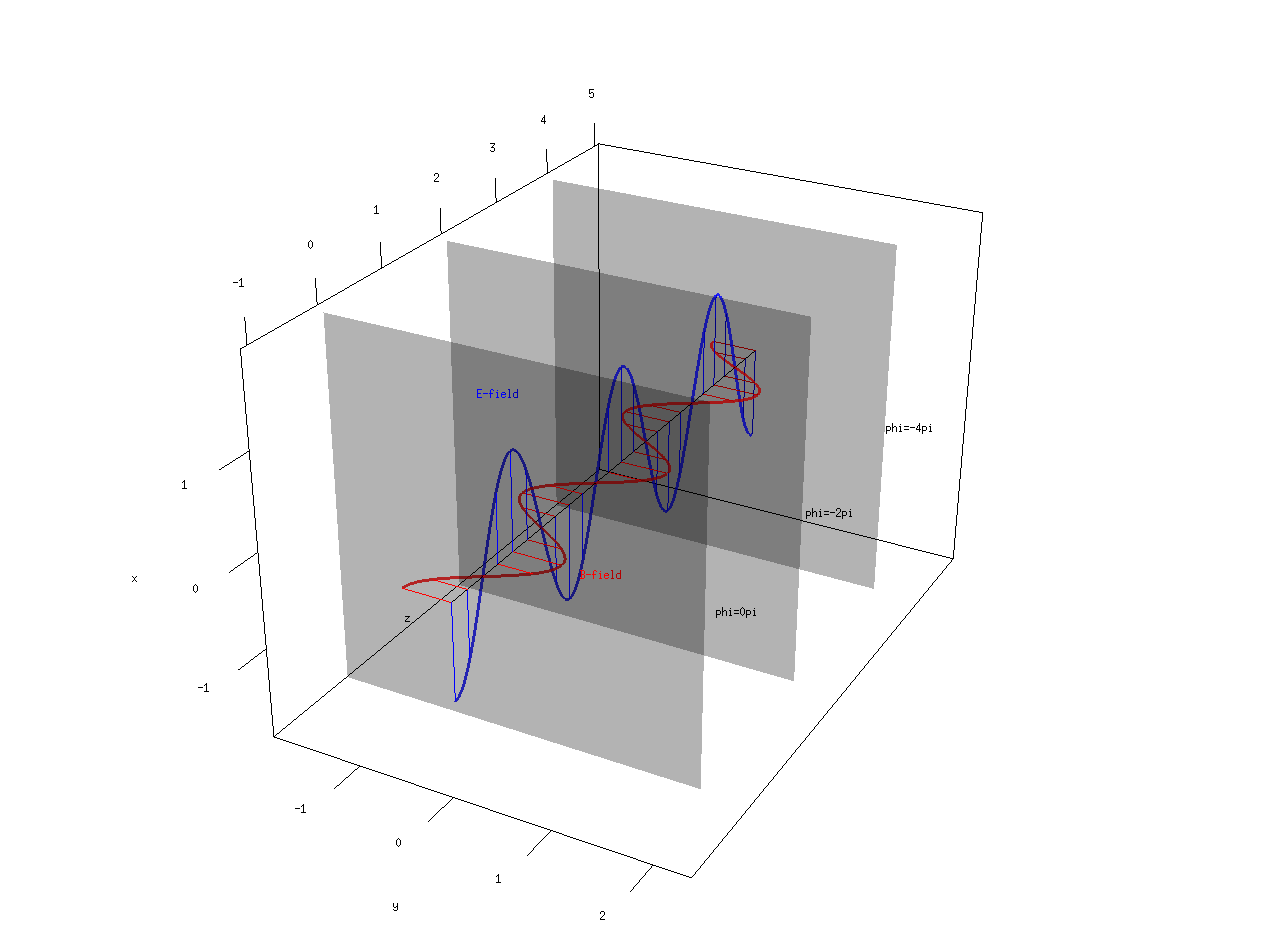
\includegraphics[width = \linewidth]{onde.png}
\caption{\textit{\textbf{Représentation d'une onde EM plane monochromatique polarisée linéairement ($\vec{E}$ vers $\hat{x}$).}}}
\end{marginfigure}

\section{Intensité d'une onde EM}  %%%%% /!\ PROFESSEURS : Avez-vous une démonstration plus complète que les slides quant à l'intensité d'une onde EM?

% AUTEUR :: Brieuc Pinon || SOURCE ::  YOUNG 13th p.1176->1178 || DATE :: 18.10.15
Quelle énergie transporte une onde électromagnétique?

Pour rappel les densités d'énergie dans le vide associées au magnitudes des champs électrique et magnétique sont 
\[u=\frac{1}{2}\epsilon_0E^{2}\]
\[u=\frac{\mu_0H^{2}}{2}\]

On sait que $\mu_0H=\frac{E}{c}=\sqrt{ \epsilon_0 \mu_0 }E$ dans le vide. On en déduit en sommant les énergies électrique et magnétique
\[u=\frac{1}{2}\epsilon_0E^{2} + \frac{1}{2\mu_0}(\sqrt{ \epsilon_0 \mu_0 }E)^{2} = \epsilon_0E^{2}\]

On remarque que les énergies associées aux champs électrique et magnétique sont égales dans notre onde.

L'énergie transportée par une onde électromagnétique peut être exprimée en fonction de la densité d'énergie, de sa vitesse et de la surface qu'elle traverse comme suit (avec A la surface perpendiculaire au déplacement de l'onde et c la célérité)
\[dU=udV=(\epsilon_0E^{2})Ac dt\]

Que l'on peut écrire sous forme d'un débit d'énergie par seconde par unité de surface (soit des $\frac{W}{m^{2}}$), que l'on appelle S
\[S=\frac{1}{A}\frac{dU}{dt}=\epsilon_0cE^{2}\]
ou en substituant $c$ par $1/\sqrt{\epsilon_0 \mu_0}$
\[S=\frac{EB}{\mu_0}\]

\begin{figure}
	\centering
	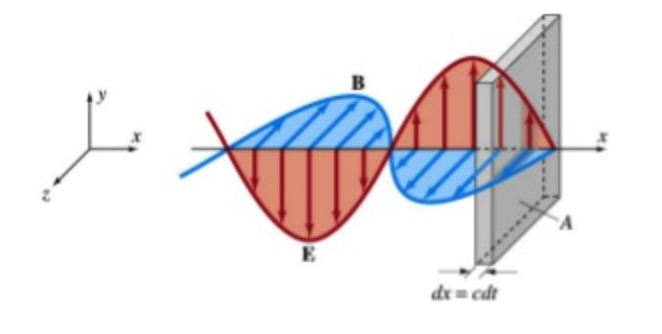
\includegraphics[height = 80pt, width = 200pt]{poynting.png}
	\caption{Vecteur de Poynting}
	\label{poynting}
\end{figure}

Afin de pouvoir l'utiliser en pratique avec des surfaces, on doit le définir sous forme d'un vecteur dont la direction et le sens sont ceux de propagation. On choisit évidemment $S$ comme norme.
\[\vec{S}=\vec{E} \times \vec{H} \]
Ce vecteur est le vecteur de \textit{\textbf{Poynting}} (vecteur \textit{normal} au pavé : voir figure \ref{poynting}), ici défini dans le vide.
Ce nouveau vecteur nous permet de définir la puissance passant à travers une surface comme
\[P=\oint_{S}\vec{S} \cdot d\vec{A}\] %%%% /!\ PROFESSEURS le Young prend une surface fermée mais ça ne parait pas très générale comme expression, l'expression est-elle correcte pour une surface ouverte?

Cette expression n'est pas encore très pratique en application directe car nos champs électromagnétiques varient dans le temps (faut-il le rappeler?). La moyenne de $S$ parait un choix plus judicieux dans nos applications, nous appelons cette moyenne l'intensité de l'onde électromagnétique. L'intensité dépend de la fonction d'onde dans le cas  d'une fonction sinusoïdale, nous obtenons (rappel: $\int_0^{2\pi} \sin^{2}(x) \, dx = \frac{1}{2}$)

\[I_{moy} = S_{av} = \frac{ E_{max} H_{max}}{2} = \frac{E_{max}^{2}}{2\mu_0c} = \frac{1}{2} \sqrt{\frac{\epsilon_0}{\mu_0}} E_{max}^{2} = \frac{1}{2}\epsilon_0 c E_{max}^{2}\]
toujours en $\frac{W}{m^{2}}$.

Tous les résultats peuvent facilement être adaptés dans des milieux de propagation non-vides. Il est nécessaire d'appliquer les substitutions $\epsilon_0 \rightarrow \epsilon$, $\mu_0 \rightarrow \mu$ et $c \rightarrow v $.

%%%% COMMENT écrire directement sous cette forme les équations?


%%%%%/!\ COMMENT cette partie est en doublon supprimer/fusionner? 
%%%%% /!\  OUI effectivement :) 
%Nous n'avons malheureusement pas trouvé de démonstration %convaincante à ce sujet. \\
%Pour rappel, nous définissons que l'\textit{intensité %maximale} d'une onde EM, c'est à dire 
%le produit de sa densité d'énergie maximale par sa vitesse, vaut ....

Notons encore que dans certains exercices, il peut être intéressant de connaitre la valeur maximale à l'instant $t$ de cette intensité. Elle vaut simplement le double de $I_{moy}$ si la fonction d'onde concernée est de type \textit{sinuosïdale}. 

\[I_{max} = \epsilon c E_{max}^{2} = \sqrt{\frac{\epsilon}{\mu}}E_{max}^{2} = \sqrt{\frac{\mu}{\epsilon}}H_{max}^{2} = E_{max} H_{max} \hspace{5pt} [W/m^{2}]\]


% Etant donné que la moyenne d'un sinus au carré (car $\vec{E}$ %et $\vec{H}$ sont très souvent exprimés de cette manière) %vaut $\frac{1}{2}$

%\[I_{moy} = \epsilon c \frac{E_{max}^{2}}{2} = %\sqrt{\frac{\epsilon}{\mu}}\frac{E_{max}^{2}}{2} = %\sqrt{\frac{\mu}{\epsilon}}\frac{H_{max}^{2}}{2} = ù\frac{E_{max} H_{max}}{2} \hspace{5pt} [J/m^{2}]\] 

	%%%%%% /!\ AUTHOR : Guillaume Van Dessel || DATE : 19.10.2015 
\chapter{Ondes mécaniques et acoustiques} 

Ce troisième chapitre est consacré aux ondes dites \textit{\textbf{mécaniques}}. Nous verrons ainsi toutes les analogies entre ondes EM et ondes mécaniques ainsi que certaines différences qui subsistent entre ces deux types d'onde.

Il est important de mentionner que les ondes EM se propagent sans l'aide d'un \textit{support matériel}, c'est là leur grande différence en comparaison avec les ondes mécaniques, qui ont besoin de «matière» pour qu'il y ait propagation. 

\section{Ondes mécaniques : Exemple de la corde vibrante}

Admettons qu'il existe une corde \textit{parfaitement souple et élastique}\footnote{Pas de couple de torsion.} dans un référentiel exempt de \textit{potentiel gravitationnel} \footnote{Ou alors dont l'effet de la pesanteur est \textit{\textbf{négligeable.}}}. La \textit{tension} longitudinale $F$ le long de la corde est supposée \textit{constante} et les déplacements longitudinaux sont considérés comme \textit{\textbf{négligeables}}.

Seuls les déplacements verticaux sont pris en compte et nous noterons : $\vec{\xi}(x,t) = y(x,t) \ \vec{a}_{y}$.

Nous admettrons aussi que lorsqu'une déformation se déplace le long de la corde, le reste de la corde n'est pas visé par la déformation et se trouve dès lors au \textit{repos} en ce sens où chacun des points du reste de la corde présente un déplacement vertical nul : $\vec{\xi}(x_{r},t) = \vec{0}$.

Considérons alors un déplacement vertical sur une portion de corde $\Delta x$ comme représenté sur la figure ci-après.  La pente de la corde dans le plan XY lorsque $\Delta x$ tend vers $0$ est donnée par $\tan (\alpha) = \frac{\partial y}{\partial x}$.

\begin{center}
	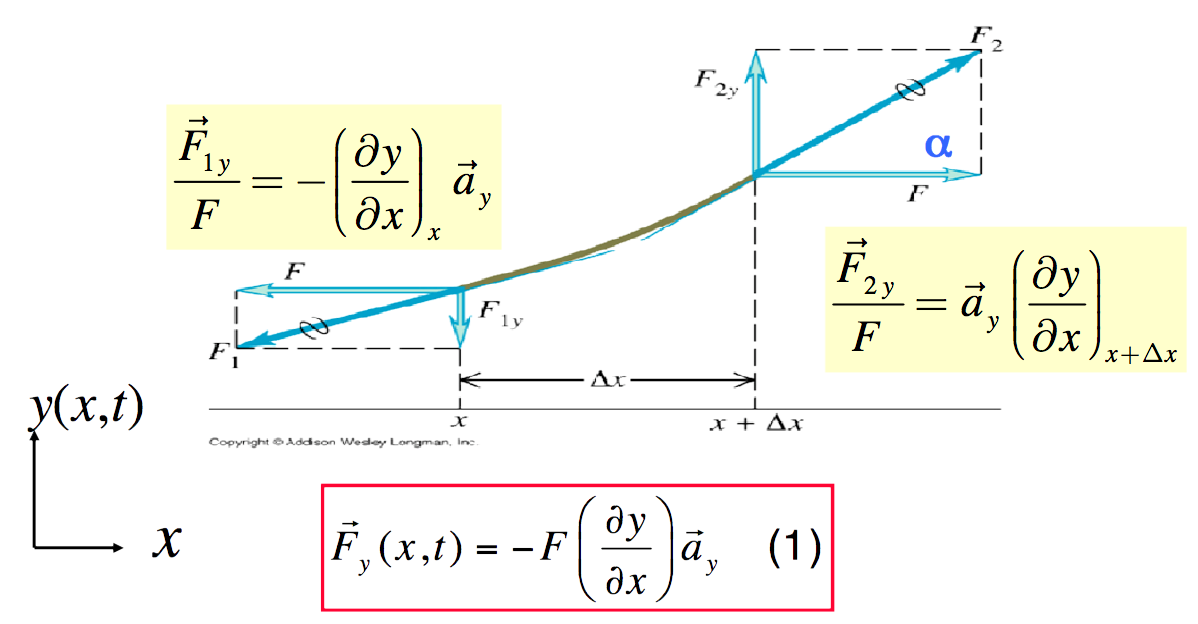
\includegraphics[width = 0.8\linewidth]{SlideCM3.png}
\end{center}

Les forces verticales en $x$ et $x+\Delta x$ valent respectivement

\begin{equation}
\vec{F}_{1y}(x,t) = - F  \left(\frac{\partial y}{\partial x}\right)_{x}  \vec{a}_{y} 
\label{Force1}
\end{equation}

\begin{equation}
\vec{F}_{2y}(x+\Delta x,t) = F \left(\frac{\partial y}{\partial x}\right)_{x+\Delta x} \vec{a}_{y}
\label{Force2}
\end{equation}

Si nous dérivons par rapport au temps, nous obtenons (en écrivant désormais $\vec{F}_{1y} = \vec{F}_{y}(x)$, puisqu'on fait tendre $\Delta x$ vers $0$, et donc qu'on s'intéresse à la force en $x$),

\begin{equation}
\frac{\partial \vec{F}_{y}}{\partial t} = - F \left(\frac{\partial^{2} y}{\partial t \partial x}\right) \vec{a}_{y} = - F \left(\frac{\partial u}{\partial x}\right) \vec{a}_{y}
\label{Force4}
\end{equation}

où $u=\frac{\partial y}{\partial t}$ est la norme de $\vec{u}(x,t)$ qui est \textbf{la vitesse verticale de déplacement d'un point de masse de la corde en fonction de sa position longitudinale $x$ et du temps $t$}.

Si nous dérivons désormais par rapport à $x$, nous obtenons une nouvelle identité intéressante : 

\begin{equation}
\frac{\partial \vec{F}_{y}}{\partial x} = -F \frac{\partial^{2} y}{\partial x^{2}} \vec{a}_{y} 
\label{ForceLOL}
\end{equation}

Établissons un bilan des forces dans la direction verticale : 

\[\sum_{i} \vec{F}_{y} = \vec{F}_{1y} + \vec{F}_{2y}  = F \left[\left(\frac{\partial y}{\partial x}\right)_{x+\Delta x} - \left(\frac{\partial y}{\partial x}\right)_{x}\right] \vec{a}_{y} \]

Étant donné que $\Delta x$ est supposé tendre vers $0$, en multipliant par $\Delta x$ en haut et en bas de la fraction : 

\begin{equation}
\sum \vec{F}_{y} \Rightarrow \lim_{\Delta x \to 0}  F \Delta x \frac{\left(\frac{\partial y}{\partial x}\right)_{x+\Delta x} - \left(\frac{\partial y}{\partial x}\right)_{x}}{\Delta x} \vec{a}_{y} = F \Delta x \frac{\partial^{2} y }{\partial x^{2}} \vec{a}_{y} 
\label{Force5}
\end{equation}

Par la troisième \textit{loi de \textbf{Newton}}, nous égalons l'expression trouvée au produit d'une masse par une accélération (donnée par la dérivée de la vitesse):
\begin{equation}
\sum \vec{F}_{y}  = m \frac{\partial^{2} y }{\partial t^{2}} \vec{a}_{y} =  (\mu \Delta x) \frac{\partial u }{\partial t} \vec{a}_{y}  
\label{Force6}
\end{equation}
où $\mu$ est la masse linéique de la corde (masse par unité de longueur).

Nous pouvons dès lors mettre en exergue la relation liant l'équation \eqref{Force5} et l'équation \eqref{Force6} : 

\begin{equation}
\frac{\partial^{2} y }{\partial t^{2}} = \frac{F}{\mu}  \frac{\partial^{2} y }{\partial x^{2}}
\label{EqOnde}
\end{equation}

ce qui représente exactement le même type d'équation que nous avons abordé à la section précédente ! 
En effet, le scalaire $\sqrt{\frac{F}{\mu}}$ équivaut ici à la vitesse de propagation de l'onde.

De même, nous observons que nous retrouvons des \textbf{EDP couplées} en $F_{y}$ et $u$.

Afin de s'en convaincre, nous utilisons les équations \eqref{Force4}, \eqref{ForceLOL} et \eqref{EqOnde} :

\[ \frac{\partial F_{y}}{\partial t} = - F \left(\frac{\partial u}{\partial x}\right)\]

\[ \frac{\partial F_{y}}{\partial x} = -F \frac{\partial^{2} y}{\partial x^{2}} = -\mu \frac{\partial^{2} y}{\partial t^{2}} = -\mu \frac{\partial u}{\partial t} \]

La résolution de l'équation \eqref{EqOnde} s'établit de la même manière que pour les ondes EM.
 
Bien entendu, les deux grandeurs scalaires impliquées dans les équations couplées admettent cette même propriété
d'\textit{impédance caractéristique}. En effet, étant donnée leur caractéristique physique, il convient que le paramètre $\mathcal{K}$ 
dans $F_{y}(x,t) = \mathcal{Z}u(x,t) + \mathcal{K}$ soit \textit{nul}.

Nous avons alors, 

\[\frac{F_{y}(x,t)}{u(x,t)} = \mathcal{Z} = \sqrt{F\mu} \hspace{8pt} [N\cdot s / m]\]

Étant donné que la corde se déplace sous l'effet d'une force, nous pouvons conclure que $\vec{F_{y}}$ exerce un travail sur la corde. 
La puissance étant par définition un travail par unité de temps, nous avons que le produit scalaire entre la force et la vitesse de son point d'application 
donne la puissance recherchée en un temps et un point donné sur l'axe :
\[P(x,t) = \vec{F}_{y}(x,t) \cdot \vec{u}(x,t) \]
Comme $\vec{F}_{y}$ et $\vec{u}$ ont la même direction, nous écrirons alors dans ce cas : 
\[ P(x,t) = F_{y}(x,t) u(x,t) = \mathcal{Z} u^{2}(x,t) = \sqrt{F \mu}\: u^{2}(x,t) = \frac{F_{y}^2(x,t)}{\mathcal{Z}}\]
Si nous considérons que le signal de l'onde mécanique le long de la corde est de \textit{type sinusoïdal}, 
nous pouvons entreprendre de calculer la valeur moyenne (sur une période) de la puissance de l'onde. 

Soit donc $\vec{y}(x,t) = \xi_{0} \cos(kx-\omega t) \vec{y}$ et dès lors $\vec{u}(x,t) = \omega \xi_{0} \sin(kx-\omega t) \vec{y}$, la \textit{valeur moyenne de ce signal \textbf{au carré}} sur un nombre entier de périodes vaut $\frac{\xi_{0}}{2}$, dès lors : 
\[ \overline{P(x,t)} = \frac{\mathcal{Z} u^{2}_{max}}{2} = \frac{\omega^{2} \xi_{0}^{2}}{2} \mathcal{Z}\]
Nous pouvons aussi définir des concepts comme celui d'\textit{énergie cinétique} de la corde en un \textit{tronçon infinitésimal} et un temps donnés.

Cette énergie cinétique vaut le produit de la masse de ce très petit tronçon, considéré comme un point de masse équivalente au tronçon, et du carré de sa vitesse
verticale en $t$. 
\[\Delta U_{k}(x,t) = \frac{(\mu \Delta x)u^{2}(x,t)}{2} \] 
La valeur maximale de cette expression (par unité de longueur) se donne par la relation : 
\[U_{k,max} = \frac{\mu u_{max}^{2}}{2}\]
Nous définissons encore le concept d'énergie \textit{potentielle de déformation} comme l'énergie du couple de forces $\vec{F}_{1y}$ et $\vec{F}_{2y}$, obtenue en multipliant la force verticale par la variation de l'angle $\alpha$
\[\Delta W = (F_{y}(x,t) \Delta l)(-\Delta \alpha)= F_{y}(x,t) \Delta l \frac{\Delta F_{y}(x,t)}{F} \]
\[\hspace{2cm} \Delta W = \frac{\Delta l}{F} \int_{0}^{F_{y}(x,t)} F_{y'} \ \mathrm{d}F_{y'} = \frac{F_{y}^{2}(x,t)}{2F}\Delta l \]

Encore une fois, la valeur maximale de cette expression (par unité de longueur) s'écrit :
\[U_{p,max} = \frac{F_{y,max}^{2}}{2F}\]
Nous remarquons alors que ces deux valeurs sont \textit{équivalentes} ! 
\\ En effet, comme $F_{y}^{2}(x,t)  = \mathcal{Z}^{2} u^{2}(x,t)$, nous pouvons écrire 

\[ U_{k,max} = \frac{\mu u_{max}^{2}}{2} =   \frac{\mathcal{Z}^{2} u_{max}^{2}}{2F} = \frac{F_{y,max}^{2}}{2F} = U_{p,max}\]

A titre de complément\footnote{Image tirée de l'adresse suivante : \url{https://ccrma.stanford.edu/realsimple/lab_inst/img31.png}}, voici la \textit{distribution de l'énergie d'une corde vibrante soumise à un \textbf{amortissement de son amplitude}} (le \textit{frottement }dissipant de l'énergie en chaleur peut être une cause de l'atténuation) : 
\begin{center}
	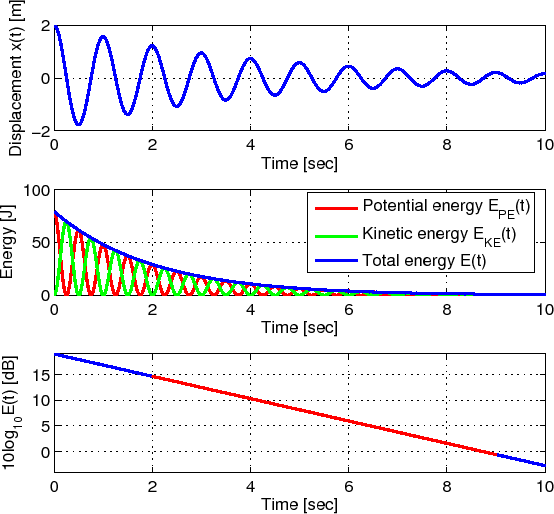
\includegraphics[width = \linewidth]{BIG.png}
\end{center}

\section{Ondes acoustiques}

Etant donnée la complexité apparente du phénomène en 3D, nous allons aborder ici le cas simplifié et \textit{\textbf{moins général}} d'une 
\textit{onde acoustique} 1D. A nouveau, nous parlons ici d'une onde \textit{\textbf{mécanique}}, c'est à dire qu'elle nécessite un support physique afin 
de pouvoir se propager dans l'espace. Cependant, nous la distinguons du cas de la corde vibrante de la section précédente à ce point-ci près; 
elle est non plus \textit{transversale}, mais bien \textit{\textbf{longitudinale}}. Les déformations du milieu traversé par l'onde ne sont plus perpendiculaires mais 
bien dans le sens du
\textit{déplacement}
de l'onde.

\subsection{Hypothèses}

Afin de pouvoir écrire les équations qui vont suivre sereinement, il nous faut dresser une liste d'hypothèses qui justifieront les écritures. 
Tout d'abord, il faudra admettre que nous travaillons avec un milieu (\textit{par exemple ici de l'air}) aux propriétés thermodynamiques \textit{parfaites}. \footnote{Source : \url{https://fr.wikiversity.org/wiki/Introduction_à_l\%27acoustique/Équation_d\%27onde}}
Nous considérons que les déplacements longitudinaux respectent la condition $L = \sqrt{DT} << \lambda$ où $\lambda$ est la longueur d'onde, $D$ le coefficient de diffusion de l'onde et 
$T$ la période de l'onde. Cette relation est vérifiée pour les basses fréquences. Ceci implique l'isentropie et l'absence de phénomènes thermodynamiques irréversibles dont l'effet sur les équations est difficilement abordable dans le cadre de ce cours. \footnote{Pour plus de formalisme, se référer à \url{https://fr.wikiversity.org/wiki/Introduction_à_l\%27acoustique/Hypothèse_acoustique}}

Dans la prochaine section, nous allons nous attarder sur le cas d'une propagation dans l'air et, sans le démontrer, accepter que ce raisonnement tienne pour la propagation dans 
d'autres milieux.

\subsection{Équations constitutives} 

Nous considérons le mouvement (en avant et en arrière) des particules  lors de la compression et de la dilatation (réversible) d'un gaz parfait dans un cylindre de section $A$. On note par $p_{y}$ la pression différentielle $\Delta p$ par rapport à la pression au repos.\\

\textbf{Loi de \textit{Newton}} : Sous forme \textit{scalaire} car la direction de déplacement des particules est supposée tout le temps horizontale et en phase avec le déplacement
de droite à gauche du piston, la loi de Newton nous fournit une relation entre la force exercée sur le gaz par le piston (la pression «\textit{locale}» aux points d'application, en notant que la pression est une force par unité de surface) et la dérivée de la vitesse des particules à ces endroits.

Nous écrirons ceci : 

$$F_{y} = -p_{y} A = m \frac{\partial{u}}{\partial t}$$ 

En notant qu'une tranche d'air d'épaisseur $\Delta x$  au repos occupe un volume $A\Delta x$, et en multipliant chaque terme par $\Delta x$, nous obtenons 
$$-p_{y} A\Delta x = \Delta x m \frac{\partial{u}}{\partial t}$$ 

Passant à  un volume \textit{infinitésimal} et définissant la masse volumique 
$\rho_{0}$ comme la masse par unité de volume, la loi de Newton se ramène à

\[\frac{\partial p_{y}}{\partial x} = - \rho_{0} \frac{\partial{u}}{\partial t}\]


\textbf{Loi de la conservation de la masse}  : Elle nous indique que si le volume diminue, la pression augmente, en vertu de la définition du module d'élasticité isostatique $B$, qui relie la pression à la variation relative de volume:
\[\Delta p  = - B \frac{\Delta V}{V} \]

Dans notre cas, $\Delta p = p_y$, $V = A \Delta x$ et $\delta V = A \Delta y$, puisque $\Delta y$ est la variation de largeur de la tranche d'air sous l'effet de la pression $p_y$. On obtient donc, en passant à la limite:

\[p_{y}  = - B \frac{\partial y}{\partial x}\] et en dérivant par rapport au temps,

\[\frac{\partial p_{y}}{\partial t} =  - B \frac{\partial u}{\partial x}\]


Une fois de plus, nous avons affaire à des EDP linéaires couplées du premier ordre. Il en résulte que les grandeurs physiques \textit{force} ou \textit{pression} (selon que l'on multiplie par $A$ ou non) et 
\textit{vitesse longitudinale} sont liées et vérifient l'équation d'onde. La vitesse de propagation du signal vaut donc machinalement\footnote{Si nous considérons la vitesse du son à travers un solide : $v = \sqrt{\frac{Y}{\rho_{0}}}$ où $Y$ est le module de \textit{Young}.} : $v = \sqrt{\frac{B}{\rho_{0}}}$.  Si nous travaillons bien avec des
gaz \textbf{parfaits}, nous pouvons écrire : $$p_{0} = \frac{nRT}{V_{0}}= \frac{mR^{*}T}{V_{0}} = \rho_{0}R^{*}T \Rightarrow v = \sqrt{\frac{\gamma RT}{M}}$$ où $M$ est la \textit{masse molaire} du gaz.

Prenons le cas de l'air, $\gamma$ est considéré comme une constante (voir \textit{Transformations adiabatiques réversibles}) et vaut approximativement $1.4$. $M$ vaut à peu près $\SI{0.02896}{[kg/mol]}$. Nous avons alors une expression approchée de la \textit{vitesse du son dans l'air} à température $T$. 
\[ v \simeq \sqrt{\frac{\gamma R}{M}} \sqrt{T} \simeq 20.05 \sqrt{T} \Rightarrow \hspace{5 pt} \mbox{pour $T = \SI{293.15}{[K]}$ : } \hspace{5pt} v \simeq \SI{343.3}{[m/s]}\]

L'impédance caractérique est donnée par :
\[
    \mathcal{Z} = \frac{p_y(x,t)}{u(x,t)} = \sqrt{B\rho_0}
\]

\subsection{Puissance et intensité}

De manière analogue\footnote{Selon les unités, le cas de la \textit{corde vibrante} renseignait sur la puissance et \textbf{non} l'intensité} aux autres cas d'ondes mécaniques, nous pouvons définir l'intensité d'une onde acoustique comme le produit de son \textit{impédance caractéristique}
par la norme de la \textit{vitesse} de la déformation locale du milieu.
Nous avons alors, 
\[I(x,t) = \mathcal{Z} u^{2}(x,t) = \frac{p_{y}^{2}(x,t)}{\mathcal{Z}}\]

dans un cas \textit{sinusoïdal}%\footnote{ C'est à dire où $y(x,t) = \xi_{max} cos(kx-\omega t)$} 
, nous pouvons définir également une intensité \textit{moyenne} sur une période : \[ |I_{moy}| = \frac{\mathcal{Z} u^{2}_{max}}{2} = \frac{\sqrt{B \rho_{0}} \omega^{2} \xi_{max}^{2}}{2}\]

Notons que $\mathcal{Z}$ dépend de facteurs thermodynamiques comme la température, c'est pourquoi nous pouvons écrire aussi sous une autre forme l'intensité moyenne en fonction de
la pression maximale locale : 
\[ |I_{moy}| = \frac{p_{max}^{2}}{2 \mathcal{Z}} \Rightarrow \hspace{5pt} \mbox{pour $T = 293.15[K]$ , $ 2 \mathcal{Z} \simeq 825.6$  : } \hspace{5pt} I_{moy} = \frac{p_{max}^{2}}{825.6}\]

\begin{center}
	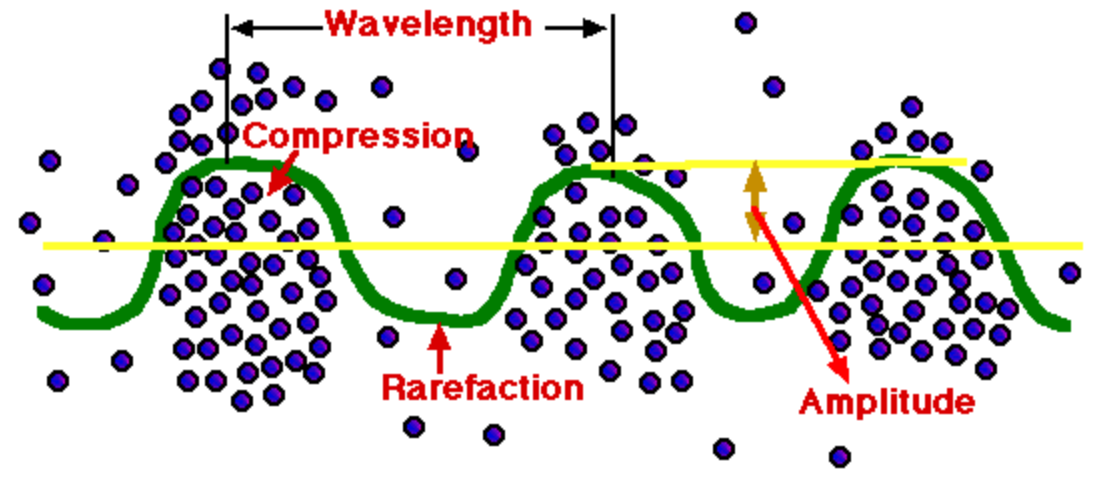
\includegraphics[width = 0.9\linewidth]{pression.png}
\end{center}

\section{Ondes planes, cylindriques et sphériques}

Nous avons introduit le \textbf{vecteur de \textit{Poynting}} à la fin de la section concernant les ondes EM. La puissance totale d'une source \textit{ponctuelle} se donne par l'expression 

\[P_{tot} = \oint \vec{S} \cdot \mathrm{d}\vec{A}\]

Dans le cas de propagations symétriques dans des configurations spéciales, nous pouvons déduire l'expression des champs électriques et magnétiques et leur \textit{décroissance} apparente, comme 
lorsque nous jetons une pierre dans une mare et voyons la propagation de type circulaire autour de la singularité. 

\subsection{Ondes sphériques} 

L'intensité perçue à une distance $r = \sqrt{x^{2} + y^{2} + z^{2}}$ de la source est proportionnelle à $\frac{1}{r^{2}}$ car la relation impliquant le vecteur de Poynting nous 
donne $P_{tot} = 4 \pi r^{2} I$. \\ 
Comme nous savons que l'intensité d'une onde EM est proportionnelle à la norme du vecteur de Poynting (de par sa définition même!), nous pouvons écrire 

\[ EH \propto \frac{1}{r^{2}} \Rightarrow E,H \propto \frac{1}{r}\]

Nous avons de manière générale, en admettant un terme \textit{d'Alembert} homogène, une expression du champ électrique : 

\[\vec{E}(\vec{r},t) = \frac{1}{r} \:f(r-vt) \:\hat{u}_{r},\] 

et pour une onde sphérique \textit{monochromatique sinusoïdale},

\[\vec{E}(\vec{r},t) = \frac{E_{0}}{r} \sin(kr-\omega t) \hat{u}_{r} = \frac{E_{0}}{r} \sin(k(r- vt)) \hat{u}_{r}, \]

où $\hat{u}_{r}$ est un vecteur unitaire dont la direction est orthogonale au vecteur de propagation (depuis le centre vers $\vec{r}$).


\subsection{Ondes cylindriques} 

L'intensité perçue à une distance $r = \sqrt{x^{2} + y^{2}}$ de la source est proportionnelle à $\frac{1}{r}$ car la relation impliquant le vecteur de Poynting nous 
donne $P_{tot} = 2 \pi r h I$.

En effet, il faut s'imaginer un exemple de source \textbf{non plus ponctuelle} mais \textit{linéique} à l'instar d'un champ magnétique à une 
distance $r$ d'un courant linéique. Chaque source ponctuelle présente sur le «fil» donne lieu à une propagation sphérique mais toutes ces propagations sphériques mises bout à bout donnent 
des \textit{fronts d'onde} sous forme d'enveloppes cylindriques concentriques autour de ce même «fil» de source linéique. Si nous imaginons un «fil» infini, à la limite,
nous avons bien la relation liant la puissance totale à l'enveloppe d'un cylindre de hauteur $h$. Si le fil est fini, cette relation est une approximation tout à fait valable sauf 
aux bords.

Comme nous savons que l'intensité d'une onde EM est proportionnelle à la norme du vecteur de Poynting (de par sa définition même!), nous pouvons écrire 

\[ EH \propto \frac{1}{r} \Rightarrow E,H \propto \frac{1}{\sqrt{r}}\]

Nous avons de manière générale, en admettant un terme \textit{d'Alembert} homogène, une expression du champ électrique : 

\[\vec{E}(\vec{r},t) = \frac{1}{\sqrt{r}} f(r-vt) \hat{u}_{r},\] 

et pour une onde cylindrique \textit{monochromatique sinusoïdale},

\[\vec{E}(\vec{r},t) = \frac{E_{0}}{\sqrt{r}} \sin(kr - \omega t) \hat{u}_{r} = \frac{E_{0}}{\sqrt{r}} \sin(k(r - v t)) \hat{u}_{r}\]

où $\hat{u}_{r}$ est ici un vecteur unitaire dont la direction est orthogonale au vecteur de propagation (depuis la projection orthogonale de $\vec{r}$ sur la source linéique jusqu'à $\vec{r}$ lui-même).


\subsection{Ondes planes} 

Le cas d'une propagation plane tout comme celui d'une propagation cylindrique est «\textit{idéal}» et n'est pas réellement envisageable physiquement.

Quoi qu'il en soit, nous pouvons tout de même faire l'expérience d'esprit qu'une onde puisse, pour tous les $\vec{r}$ présents sur un plan dont la normale est la direction 
de propagation, avoir la même intensité pour ses composantes (champ électrique ou magnétique). Nous y reviendrons à la prochaine section.

Dans ce cas-là, toute la puissance est \textit{partagée} à chaque fois sur chaque même plan infini (ils sont parallèles entre eux) et nous \textbf{n'observons plus} de décroissance 
en $1/r^{n}$! Nous écrivons alors simplement les relations suivantes : 
\[E,H \propto 1\]
\[\vec{E}(\vec{r},t) = E_{0} \sin(\vec{r}\cdot \vec{k}-\omega t) \hat{u}_{r}\]

où $\hat{u}_{r}$ est un vecteur unitaire dont la direction est orthogonale au vecteur de propagation.

\section{Effet Doppler}

Considérons des référentiels galiléens et \textit{négligeons les effets relativistes}. 
Si la source d'une onde ou bien son observateur se déplacent l'un par rapport à l'autre, l'observateur, malgré une \textit{pulsation identique}, verra les fronts d'onde avec une fréquence différente de celle de la source!

Nous allons uniquement étudier ce phénomène en régime dit «\textit{stationnaire}» car si la fréquence de la source varie ou que la vitesse de la source varie ou que celle-ci 
passe à proximité directe de l'observateur et le dépasse, l'observateur aura droit à une phase «\textit{transitoire}» qui ne respectera pas à la lettre la loi que nous allons énoncer.

Nous garderons à l'esprit qu'une vitesse \textbf{positive} est une vitesse dans le sens \textit{source $\rightarrow$ observateur}.

L'effet Doppler est décrit par l'équation suivante, à vitesses $v_{o}$ et $v_{s}$ constantes et dans un même milieu de propagation (vitesse de l'onde $v$ constante) : 

\[f_{o} = \frac{v-v_{0}}{v-v_{s}}f_{s}\]

On peut écrire cette relation sous la forme
$$ f_{o} = f_s\Big(1+\frac{v_s-v_{0}}{v-v_{s}}\Big)$$
Dans le cas où $v_{o},v_{s} \ll v$, le terme $v-v_s$ vaut approximativement $v$ et nous ramenons l'égalité précédente à 

\[f_{o} \simeq f_{s} (1 + \frac{\Delta v_{s,o}}{v}) \]
avec $\Delta v_{s,o}=v_s-v_0$.

\textbf{Notons} toutefois la version \textit{relativiste} de l'effet Doppler, d'application traditionnellement lorsque $v \geq 10^{-1} c$ : 
\[  f_{o} = \sqrt{\frac{c-v}{c + v}} f_{s}\]

\begin{figure*}
	
\includegraphics[width = 0.65\linewidth]{doppler.png}
\end{figure*}

\section{Principe de l'intensité \textit{relative} et décibels} 

Nous sommes tous familiers de près ou de loin à ce concept de \textit{décibels}. Nous en entendons parler lorsqu'il s'agit de musique et d'intensité sonore. Il faut toutefois repartir de la définition: le décibel est une unité relative, qui permet d'exprimer tout rapport de puissance (ou d'intensité) dans une échelle logarithmique:
\[ (P_2/P_1)_{dB} = 10 \log_{10}\left(\frac{P_2}{P_1}\right) \]

Par exemple, si $P_2 = 2P_1$, on dira que $P_2$ est de 3 dB supérieure à $P_1$. 

Toutefois, le décibel peut devenir une unité absolue si on fixe $P_1$ à une valeur de référence: si $P_1 = 1$ W, le rapport en décibels exprime la puissance de $P_2$ en dBW (un émetteur de 3 dBW émet 2 Watts); si $P_1 = 1$ mW, le rapport en décibels exprime la puissance de $P_2$ en dBm. 

Enfin, dans le cas du son, on peut exprimer l'intensité d'une onde acoustique en comparant l'intensité absolue à une valeur de référence égale au seuil d'audibilité de l'oreille humaine $I_0 = 10^{-12}$ W/m$^2$. Dans ce cas on parlera de dB(A), où le (A) se lit comme acoustique. L'intensité du son en dB(A) est naturellement donnée par 
\[ I_{dB(A)} = 10 \log_{10}\left(\frac{I}{I_{0}}\right) \]
A titre d'exemple, l'intensité produite par un concert de rock vaut 1 W/m$^2$, autrement dit 120 dB(A), ou encore $10^{12}$ fois plus que le seuil d'audibilité. 
\begin{marginfigure}[-5cm]
	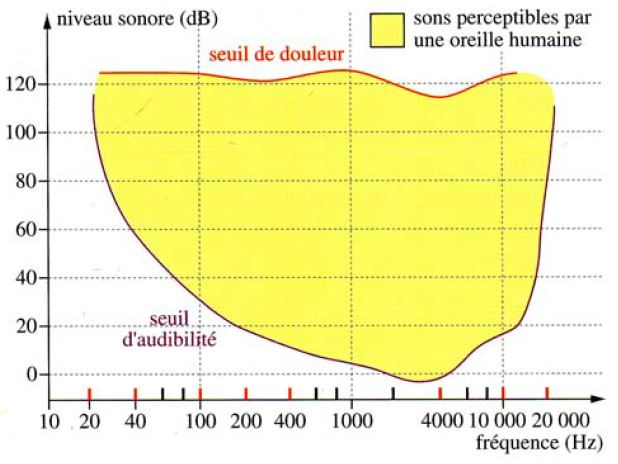
\includegraphics[width = \linewidth]{audition.jpg}
	\caption{Seuil de douleur et d'audibilité de l'oreille humaine}
\end{marginfigure}

	\chapter{Polarisation, réflexion, réfraction}

\section{Polarisation} 

La \textit{polarisation d'une onde électromagnétique} est le lieu décrit au cours du temps à un endroit donné de l'espace par l'extrémité du vecteur champ
électrique associé à cette onde. Ce concept est inhérent aux ondes \textbf{transverses}. 
Dans le cadre de ce cours, nous allons nous intéresser aux ondes EM transverses planes afin d'analyser la polarisation de l'onde "facilement" étant donné que le vecteur champ électrique sera toujours
contenu dans un plan et que les plans successifs sont tous parallèles. 

\subsection{Expression générale du champ électrique d'une onde EM transverse plane}
\begin{marginfigure}
	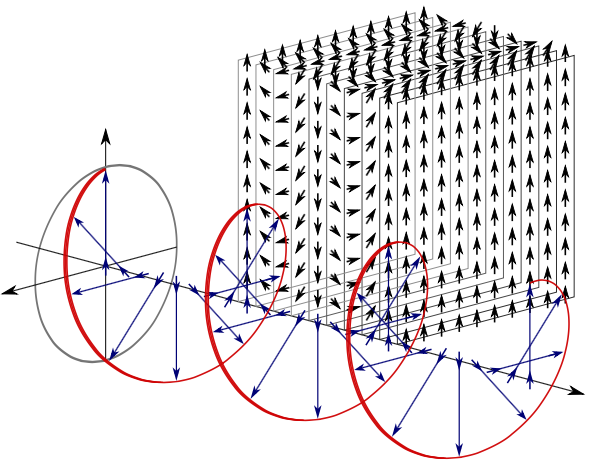
\includegraphics[width = \linewidth]{polarisationL.png}
	\caption{Illustration de la polarisation circulaire d'une onde plane Nous pouvons en effet observer que le lieu décrit par la pointe du vecteur E est un cercle.}
\end{marginfigure}
Avec la définition que nous venons de donner, nous pouvons simplement écrire (pour des plans d'équation : $ z = ||\vec{r}||$) 

\[\vec{E}(\vec{r},t) = A_{x} \sin(\vec{k}\cdot \vec{r} - \omega t) \hat{x} + A_{y} \sin(\vec{k}\cdot \vec{r} - \omega t + \phi) \hat{y}\] 

où $\vec{r} = (x,y,z)$ représente les coordonnées cartésiennes du point considéré, \\ $\phi$ est le \textbf{déphasage} angulaire entre 
la composante en Y
et la composante en X.\\

Si $A_{x},A_{y}, \phi$ 
sont quelconques, la polarisation est dite
 \textit{\textbf{elliptique}}
et cela se vérifie facilement.\\
Dans le cas particulier où $\phi = n \pi$, l'effet du déphasage n'est plus perceptible réellement car nous aurions, en fonction 
de $n$ pair ou impair, un second terme valant en norme $\pm A_{y} \sin(\vec{k}\cdot \vec{r} - \omega t)$ \\
Dès lors, nous pourrions regrouper les deux sinus en un seul dans une direction de pente 1 en X et Y car nous aurions une combinaison 
des vecteurs unitaires $\hat{x}$ et $\hat{y}$. Dans ce cas-là, la polarisation devient \textit{\textbf{linéaire}}. \\
Dans le cas particulier où $\phi = \frac{(2n+1) \pi }{2}$ \textbf{et} la valeur absolue des amplitudes $A_{x}, A_{y}$ est identique, 
nous avons affaire, par le même genre de raisonnement, à une polarisation \textit{\textbf{circulaire}} (voir image\footnote{Source: \url{https://fr.wikipedia.org/wiki/Onde_plane}}). 
En effet, le second terme devient ici un cosinus de même pulsation angulaire et son amplitude vaut $\pm A_{x}$. 



\section{Réflexion et réfraction} 


\subsection{Mise en route: réflexion et transmission d'une onde mécanique le long d'une corde} 

\begin{figure*}
	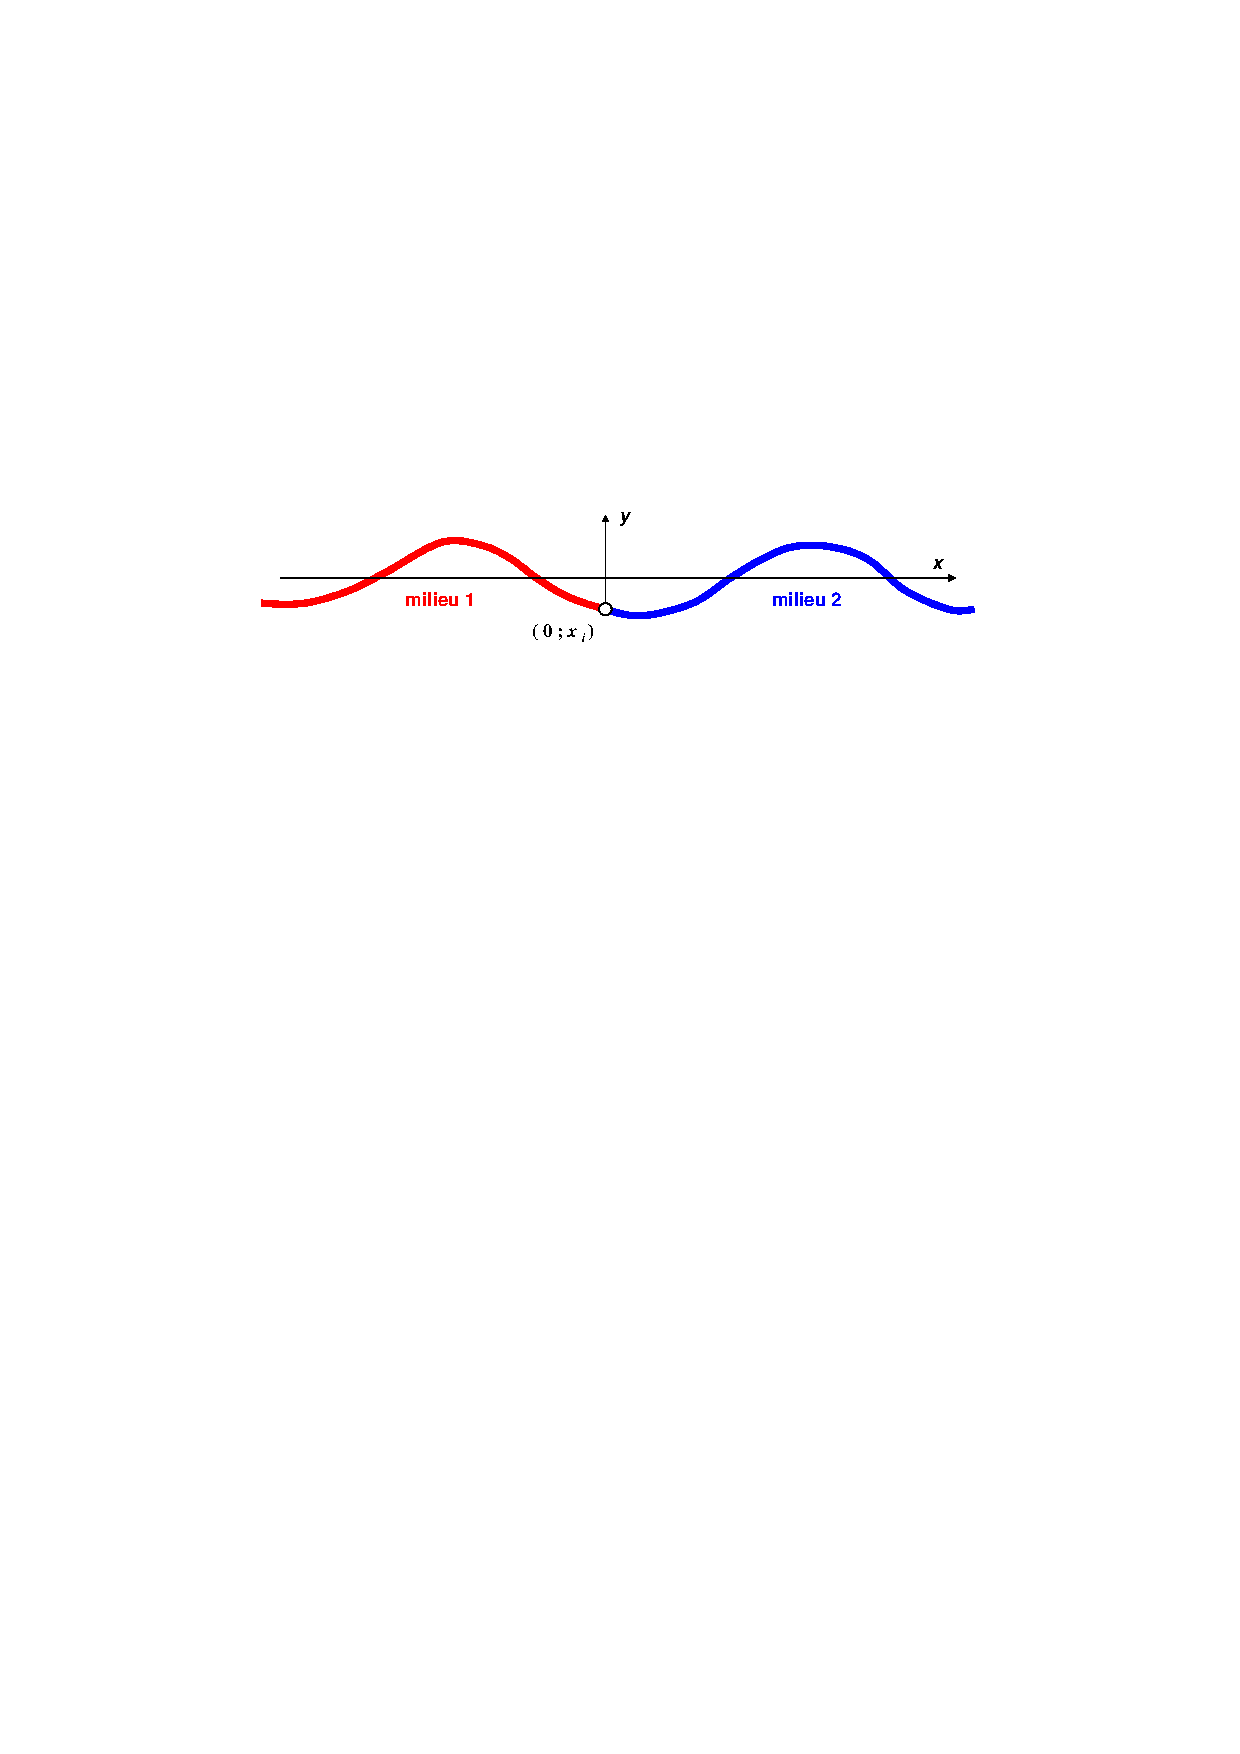
\includegraphics[width=\linewidth]{CM4_condlimite}
	\caption{L'interface de la corde tendue.}
\end{figure*}
Avant de développer le cas des ondes EM, étudions la transmission (et la réflexion qui en résulte forcément) d'une onde \textit{mécanique} transversale d'un milieu défini par les paramètres $({F}_1,{\mu_1})$ à un autre défini par $({F}_2,{\mu_2})$ (pour rappel, $F$ est la tension dans la corde et $\mu_i$, dans le contexte de la corde, représente sa masse par unité de longueur; la vitesse de phase s'exprime par $v_i = \sqrt{\frac{F_i}{\mu_i}}$, et le nombre d'onde $k_i = \omega/v_i$, $i = 1, 2$). Cette vitesse change d'un milieu à un autre.\\
L'onde \textit{incidente} (c.-à-d. l'onde avant qu'elle ne rencontre l'interface) peut s'écrire sous forme scalaire


\[ \xi_{1i}(x,t) = I \sin(k_{1}r - \omega t) \]

L'onde réfléchie et l'onde transmise auront pour équations respectives\footnote{-$k_{1}$ dénote bien que l'onde réfléchie se déplace dans la direction opposée par rapport à l'onde incidente.} : 
\[ \xi_{1ir}(x,t) = R \sin(-k_{1}r - \omega t) \]
\[ \xi_{2t}(x,t) = T \sin(k_{2}r - \omega t) \]

\textit{Les conditions aux interfaces impliquent ici la continuité du déplacement vertical de la corde $\xi$ et la continuité de la force 
verticale $F_y$}.  L'application de ces conditions de continuité résulte en un système de 2 équations à 2 inconnues $(R,T)$ :

\[\xi_{1i}(0,t) + \xi_{1r}(0,t) = \xi_{2t}(0,t) \Leftrightarrow I + R = T\]
\[F_{y,1i}(0,t) + F_{y,1r}(0,t) = F_{y,2t}(0,t) \Leftrightarrow k_{1}I - k_{1}R = k_{2}T\]

Nous obtenons trivialement pour chaque inconnue les relations suivantes : 

\[R = \frac{k_{1} - k_{2}}{k_{1} + k_{2}}I\]
\[T = \frac{2 k_{1}}{k_{1} + k_{2}}I\]

On observe que tant l'onde transmise que l'onde réfléchie dépendent des caractéristiques des deux tronçons de corde !



\subsection{Réflexion et réfraction d'une onde EM} 


Nous pouvons transposer l'analyse ci-dessus aux ondes électromagnétiques, afin de décrire leur comportement à l'interface entre un milieu 1 ($\epsilon_{1}, \mu_{1}$) et un milieu 2 ($\epsilon_{2},\mu_{2}$), chaque milieu étant caractérisé par sa \textit{\textbf{perméabilité magnétique}} $\mu_i$
et sa \textbf{\textit{permittivité électrique}} $\epsilon_i$.  \\

Pour rappel, la vitesse\footnote{Vitesse dite de \textit{phase}.} d'une onde électromagnétique vaut  

\[v = \frac{1}{\sqrt{\epsilon \mu}}\ = \frac{1}{\sqrt{\epsilon_{r} \mu_{r}}} \frac{1}{\sqrt{\epsilon_{0} \mu_{0}}} = \frac{1}{\sqrt{\epsilon_{r} \mu_{r}}} c,  \] 

et l'impédance caractéristique est définie par 

\[Z = \sqrt{\frac{\mu}{\epsilon}} = \sqrt{\frac{\mu_0\mu_r}{\epsilon_0\epsilon_r}} = Z_0 \sqrt{\frac{\mu_r}{\epsilon_r}}.  \]

On peut également définir l'indice de réfraction comme le rapport $n = c/v = \sqrt{\epsilon_{r}\mu_r}$.  \\

Une onde, lorsqu'elle passe d'un milieu à un autre, conserve sa \textbf{fréquence}. La longueur d'onde (et donc le nombre d'onde) sont quant à eux tous affectés 
par le changement de milieu car ils dépendent directement de la vitesse de l'onde.


Afin de clarifier les choses, les différentes notations que nous allons utiliser sont reprises à la figure \ref{fig_CM4_conventions_k}.
\begin{marginfigure}
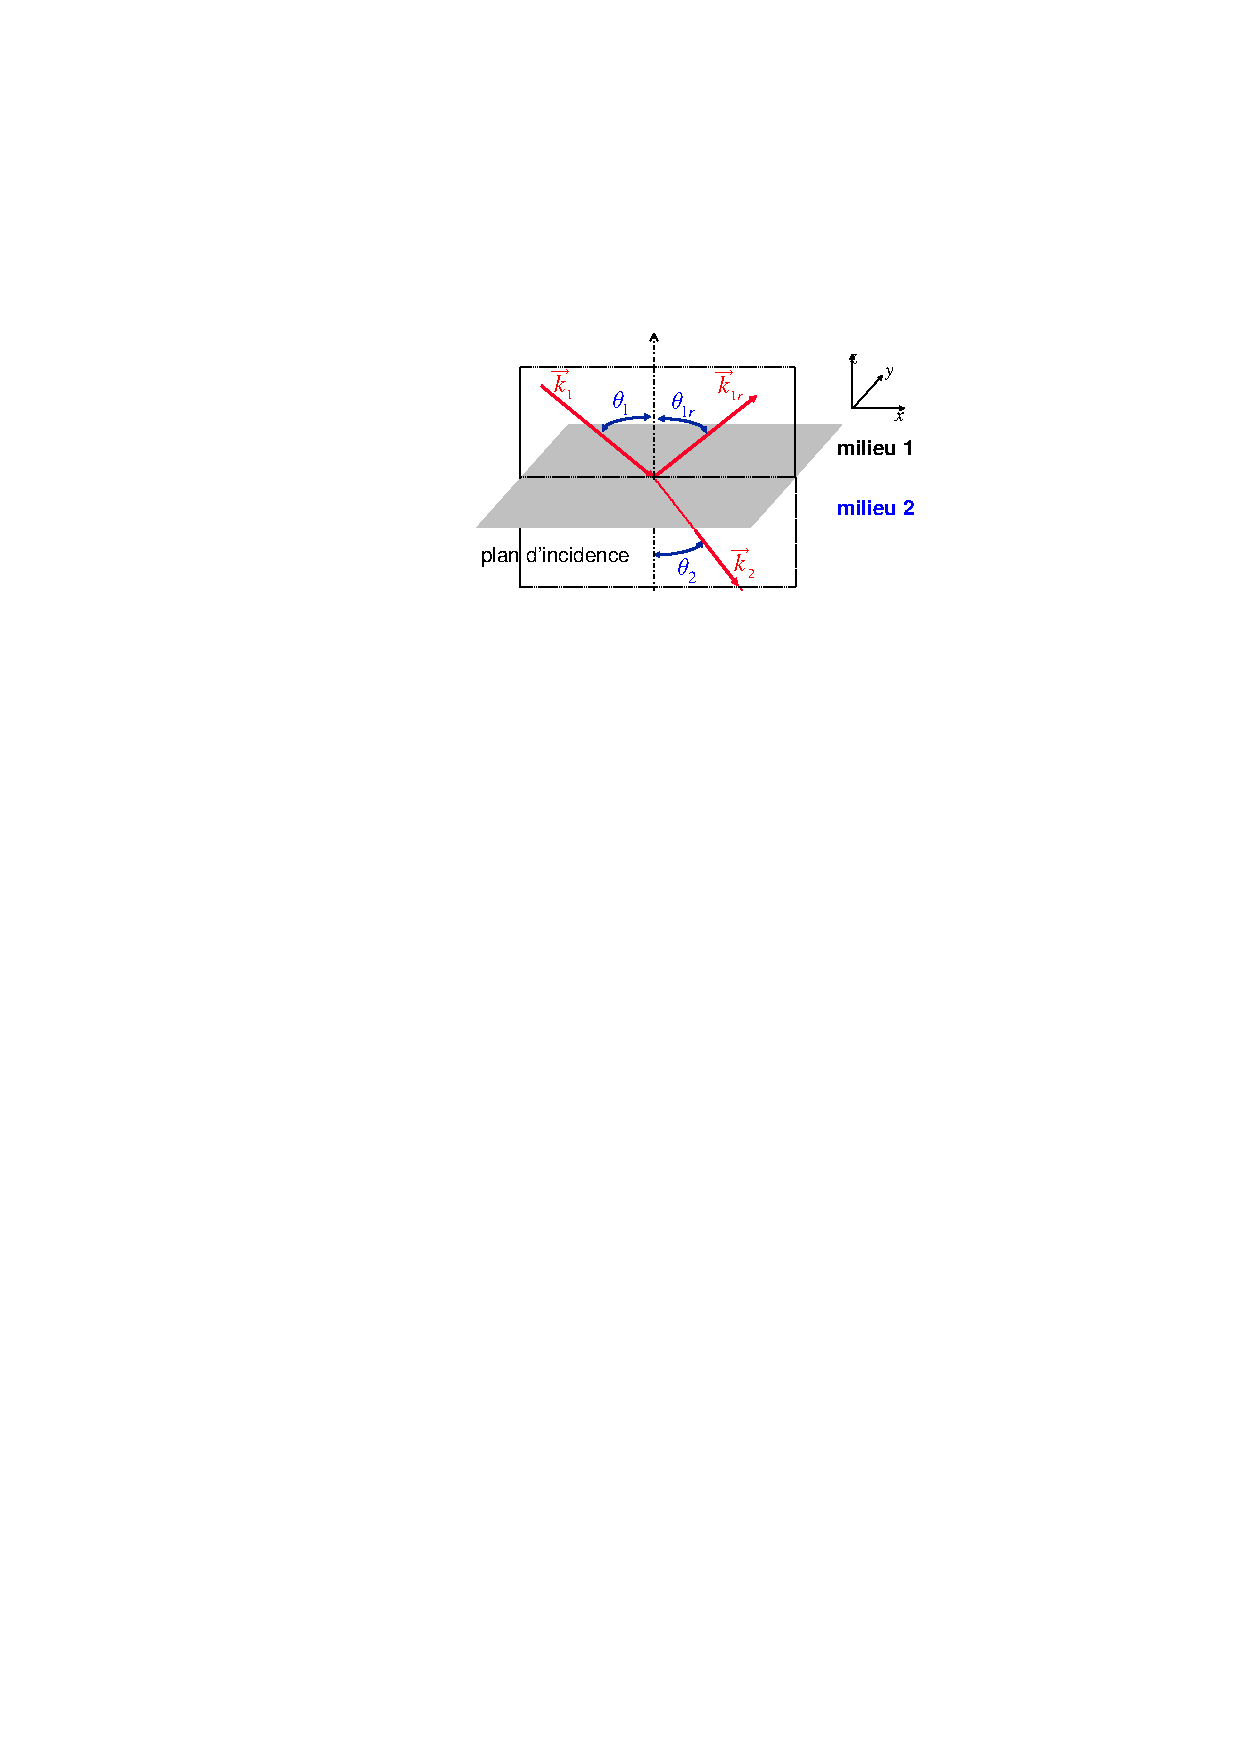
\includegraphics[width = \linewidth]{CM4_conventions_k}
\caption{Le plan d'incidence est le plan qui est formé de deux des 3 vecteurs d'ondes. (Ces 3 vecteurs d'onde sont coplanaires, le plan d'incidence sera donc la même si l'on prend le vecteur incident et réfléchi ou incident et transmis par exemple.)\\
Les caractéristiques de l'onde \textbf{incidente} seront notés avec un indice $1$ ou $1i$.\\
Les caractéristiques de l'onde \textbf{réfléchie} seront notés avec un indice $1r$ ou $r$. \\
Les caractéristiques de l'onde \textbf{transmise} seront notés avec un indice $2$ ou $2t$. \\
\textbf{Les angles sont toujours mesurés par rapport à la normale de l'interface!}}
\label{fig_CM4_conventions_k}
\end{marginfigure}

On peut tout d'abord montrer que l'angle d'\textit{incidence} vaut l'angle de \textit{réflexion}. 

\subsection{Loi de Snell}

Tout d'abord, nous avons les relations  $c = n_{1} v_{1} = n_{2} v_{2}$ et donc $\lambda_{1} n_{1}= \lambda_{2} n_{2}$.
De plus, les conditions aux interfaces imposent que la vitesse et donc le déplacement tangentiel à l'interface doit être le même. \\
Dès lors, (voir photo) les deux longueurs $L$ sont identiques. Par trigonométrie élémentaire, nous reportons les angles $\theta_{1}$ et $\theta_{2}$ 
dans les triangles rectangles et écrivons : $\mathcal{L} = \frac{\lambda_{1}}{\sin(\theta_{1})} = \frac{\lambda_{2}}{\sin(\theta_{2})}$


\begin{marginfigure}
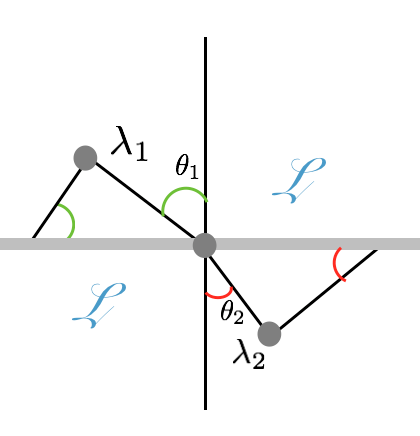
\includegraphics[width = \linewidth]{snell.png}
\caption{Illustration de la loi de Snell, les deux longueurs doivent être identiques}
\end{marginfigure}

Nous obtenons alors la \textbf{Loi de Snell}, valable pour des milieux \textit{isotropes}, transparents (non-absorbants) et linéaires (le tout à la fois!) :
\[ n_{1} \sin(\theta_{1}) = n_{2} \sin(\theta_{2})\]

Cette loi prédit les \textit{directions} des ondes réfléchies et transmises, mais ne dit rien quant à leur \textsl{amplitude} (ou leur énergie). 

\subsection{Equations de Fresnel}

Les \textbf{équations de Fresnel}, sur base des conditions aux interfaces pour les champs électriques et magnétiques, permettent de caractériser les amplitudes des ondes réfléchies et transmises. \\ 
Il est important de se souvenir de l'\textit{impédance caractéristique} qui quantifie le rapport des normes des champs électriques et magnétiques. Nous allons traiter uniquement du cas le plus courant, celui des ondes planes \textit{transverses}, afin de faciliter la compréhension de cette matière\footnote{Un raisonnement analogue peut-être entrepris concernant les ondes longitudinales. \\Enormément de paramètres seraient inversés et les conditions de continuité seraient différentes.}. \\

Tout d'abord, la relation permettant de calculer (de \textit{manière générale} ici) un champ en fonction de l'autre\footnote{Par convention, la direction de $\vec{H}$ est ($\hat{k} \times \vec{E}$) et la direction de $\vec{E}$ est 
($ \vec{H} \times \hat{k}$) } : 

\[\vec{H}(\vec{r},t) = \frac{1}{Z}\vec{1_k} \times \vec{E}(\vec{r},t) \]%= \frac{n}{c\epsilon}\vec{H}(\vec{r},t) = \frac{c\mu}{n}\vec{H}(\vec{r},t)\]

Nous pouvons alors décomposer ce dernier en une composante \textit{parallèle} au plan d'incidence et une autre \textit{perpendiculaire} à ce dernier. La composante appartenant au plan d'incidence peut elle même être décomposée comme montré sur la figure \ref{decomp}, dans le plan $xz$.\\ 

Nous pouvons décomposer chaque onde selon trois composantes polarisées linéairement dans les directions $\hat{x}, \hat{y}, \hat{z}$ sur la figure. \\
Dès lors, nous allons pouvoir réappliquer les concepts vus avec la corde vibrante concernant l'amplitude de chacune de ces composantes. Il est avant tout important de spécifier les conventions prises pour la suite. Celles-ci sont précisées aux figures \ref{fig_convention1}, \ref{fig_convention2} et \ref{decomp}.
\begin{marginfigure}[-4cm]
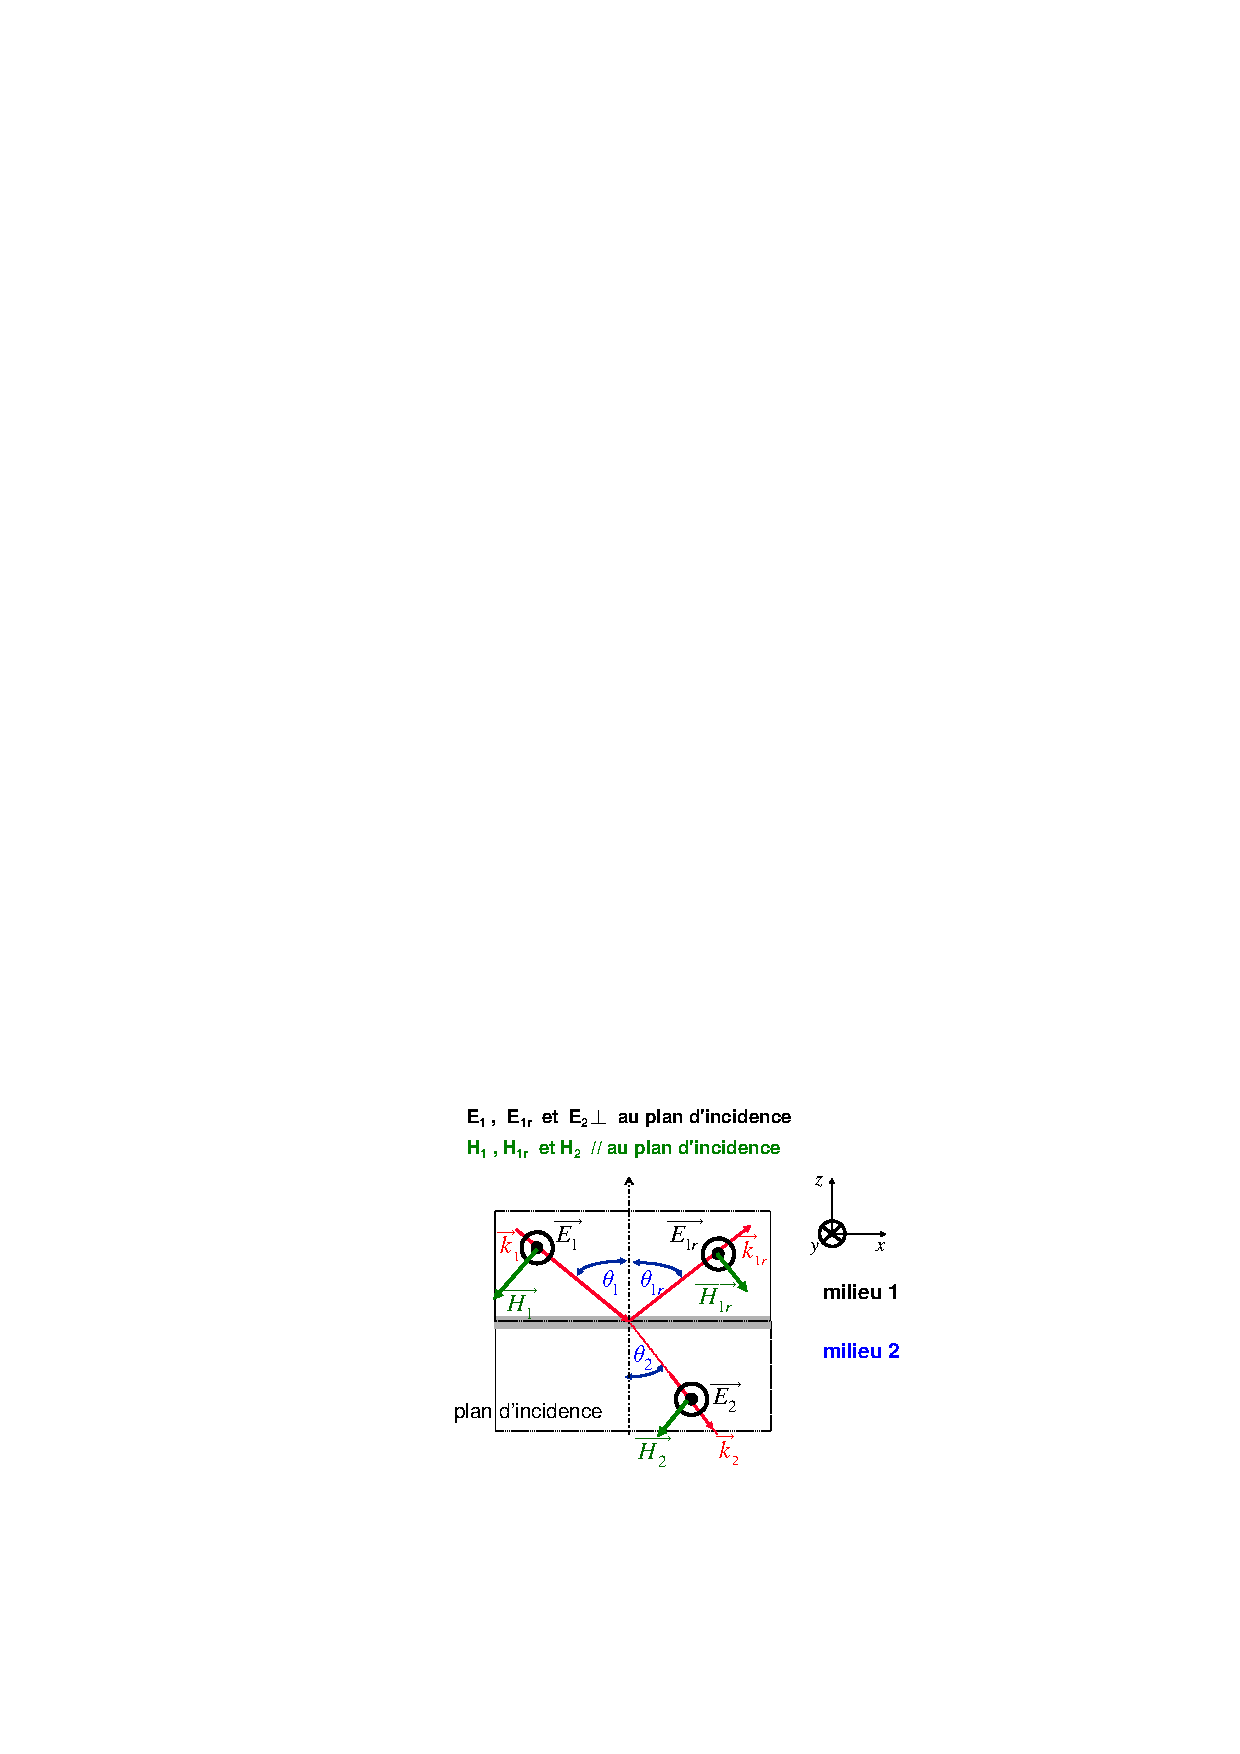
\includegraphics[width=\linewidth]{convention1}
\caption{Convention prise pour les champs électriques incidents parallèles à l'interface}
\label{fig_convention1}
\end{marginfigure}
\begin{marginfigure}
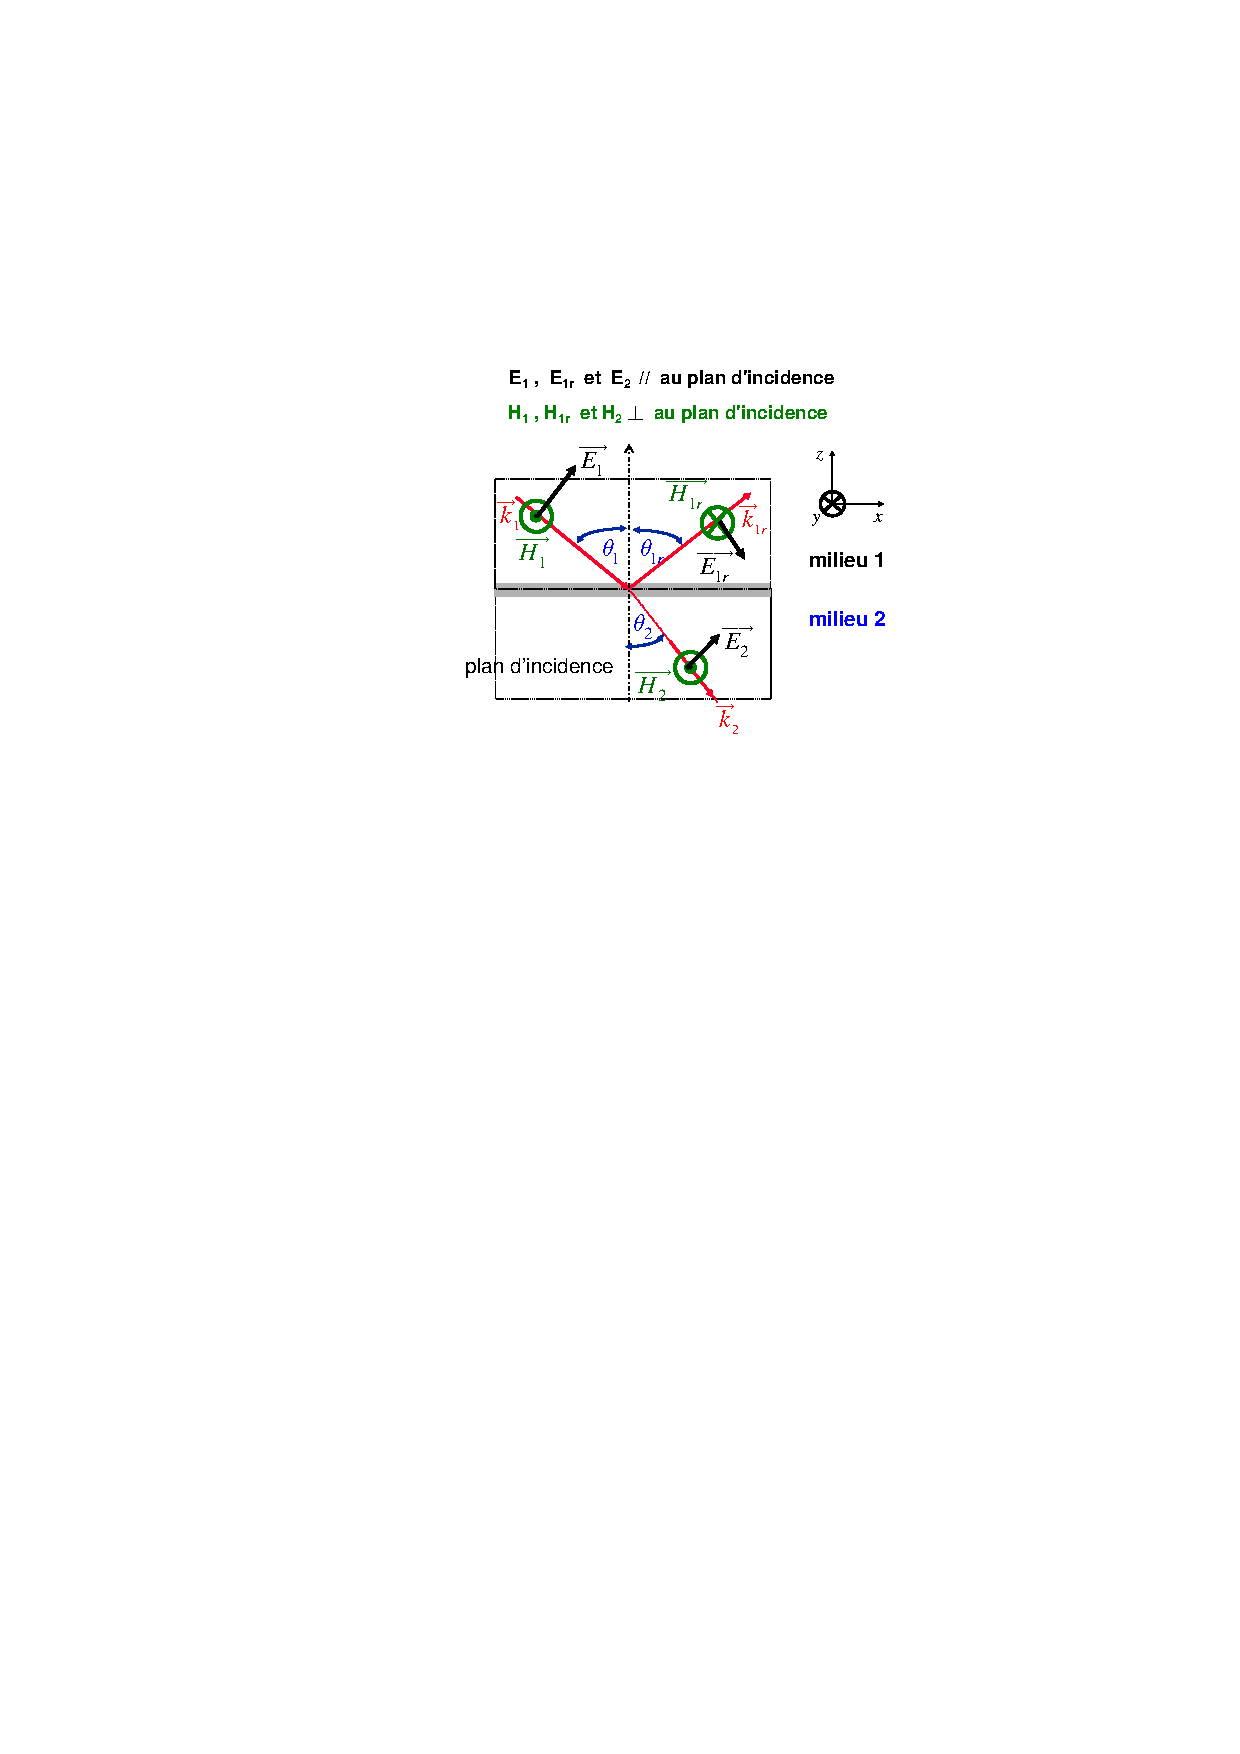
\includegraphics[width=\linewidth]{convention2}
\caption{Convention prise pour les champs H incidents parallèles à l'interface}
\label{fig_convention2}
\end{marginfigure}
\begin{marginfigure}
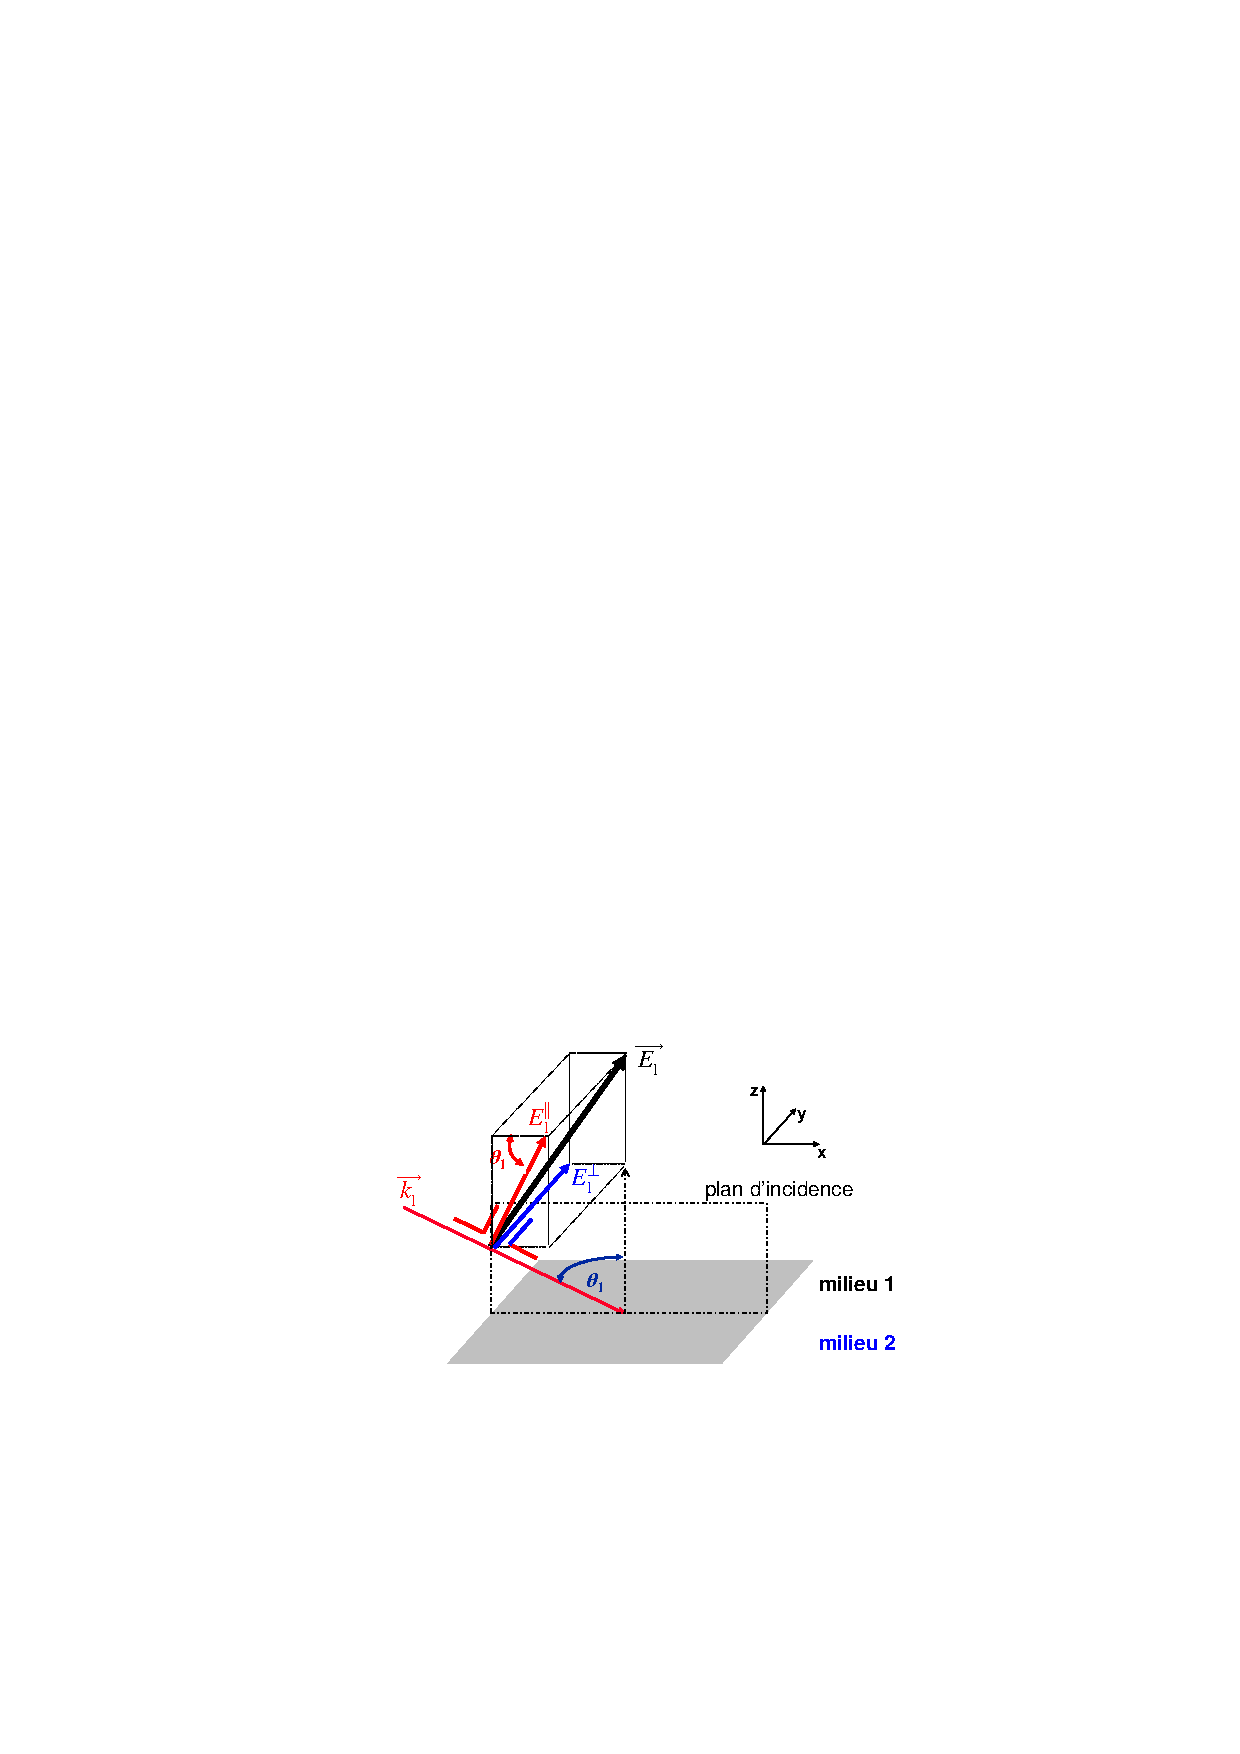
\includegraphics[width=\linewidth]{CM4_planincident}
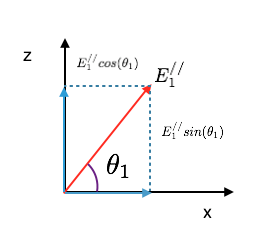
\includegraphics[width=\linewidth]{explicationsmall}
\caption{Décomposition du vecteur champ électrique par rapport au plan incident (haut) et projection du vecteur // au plan incident sur le plan xz (bas)}
\label{decomp}
\end{marginfigure}
 Commençons par écrire les ondes \textit{réfléchie} et \textit{transmise} en fonction de l'onde \textit{incidente}.\\
\textbf{Incidente:} $$ \vec{E}_{1i} (\vec{r},t) = (E^{\parallelsum}_{1i} \cos(\theta_{1})  \hat{x} + E_{1i}^{\perp} \hat{y} + E_{1i}^{\parallelsum} \sin(\theta_{1}) \hat{z} ) \sin(\vec{k}_{1i}\cdot \vec{r} - \omega t) $$  
\textbf{Réfléchie:}  $$ \vec{E}_{1r} (\vec{r},t) = (E^{\parallelsum}_{1r} \cos(\theta_{1})  \hat{x} + E_{1r}^{\perp} \hat{y} - E_{1r}^{\parallelsum} \sin(\theta_{1}) \hat{z} ) \sin(\vec{k}_{1r}\cdot \vec{r} - \omega t) $$
\textbf{Transmise:}$$ \vec{E}_{2t} (\vec{r},t) = (E^{\parallelsum}_{2t} \cos(\theta_{2})  \hat{x} + E_{2t}^{\perp} \hat{y} + E_{2t}^{\parallelsum} \sin(\theta_{2}) \hat{z} ) \sin(\vec{k}_{2t}\cdot \vec{r} - \omega t) $$ 

 
Notons que $\vec{k_{1r,z}} = - \vec{k_{1i,z}}$ et que $\vec{k_{2t}}$ prolonge l'angle de \textit{réfraction} en ayant, pour rappel, une norme de $\frac{\omega}{v_{2}}$.
Notons également que résoudre le problème pour le champ électrique nous permettra également de calculer le champ magnétique par la relation énoncée plus haut.
Toutefois, il nous faut également les expressions des champs $\vec{H}(\vec{r},t)$ afin de posséder assez d'équations.

Etant donné que $\hat{k_{1i}} = (\sin(\theta_{1}),0,-\cos(\theta_{1})) $, l'expression du champ magnétique incident se calcule et donne :
\begin{equation*}
\begin{split}
\vec{H}_{1i}(\vec{r},t)& = \frac{1}{Z_1} (\hat{k_{1i}} \times \vec{E}_{1i}(\vec{r},t))\\ &= \frac{1}{Z_1} \sin(\vec{k}_{1i}\cdot \vec{r} - \omega t)(E^{\perp}_{1i}\cos(\theta_{1}) \hat{x} - E^{\parallelsum}_{1i} \hat{y} + E^{\perp}_{1i}\sin(\theta_{1}) \hat{z} )
\end{split}
\end{equation*}
Les ondes incidente, réfléchie et transmise sont donc :\\ 
\textbf{Incidente} $$ \vec{H}_{1i} (\vec{r},t) = (E^{\perp}_{1i}\cos(\theta_{1}) \hat{x} + E^{\parallelsum}_{1i} \hat{y} + E^{\perp}_{1i}\sin(\theta_{1}) \hat{z} ) \frac{1}{Z_1} \sin(\vec{k}_{1i}\cdot \vec{r} - \omega t)$$

\textbf{Réfléchie} $$ \vec{H}_{1r} (\vec{r},t) = (-E^{\perp}_{1r} \cos(\theta_{1})  \hat{x} - E_{1r}^{\parallelsum} \hat{y} + E_{1r}^{\perp} \sin(\theta_{1}) \hat{z} ) \frac{1}{Z_1} \sin(\vec{k}_{1r}\cdot \vec{r} - \omega t) $$

\textbf{Transmise} $$ \vec{H}_{2t} (\vec{r},t) = (E^{\perp}_{2t} \cos(\theta_{2})  \hat{x} - E_{2t}^{\parallelsum} \hat{y} + E_{2t}^{\perp} \sin(\theta_{2}) \hat{z} ) \frac{1}{Z_2}\sin(\vec{k}_{2t}\cdot \vec{r} - \omega t) $$
 
Nous abordons alors réellement les équations de Fresnel.
%\footnote{Si vous désirez de plus amples informations sur ce qui a été dit et tout ce qui suivra, vous pouvez consulter le site suivant : \url{http://www.edu.upmc.fr/physique/phys325/Documents/Reflexion-Refraction.pdf}.}.
 La somme vectorielle des champs électriques en $\hat{x}$ 
du milieu 1 (à savoir ceux dans cette même direction pour l'onde incidente et réfléchie) doit être équivalente à celle du milieu 2 (à savoir l'onde transmise).%DONE\todo{CORRIGER LE SCHEMA : Ne respecte pas les conventions des slides (pages 16 et 17 CM4) le reste a été adapté. Mettre a la place du schema les fig 1 et 2 issues des slides, elles sont les plus adaptées}

%%% PROFESSEURS : Si nous plaçons un champ électrique à proximité de l'interface, jouera t'il un rôle dans la continuité de celui ci aux interfaces? Peut-on brouiller en quelque
%%% sorte ce qu'il se passe aux interfaces de quelque manière que cela soit? 

%\begin{center}
%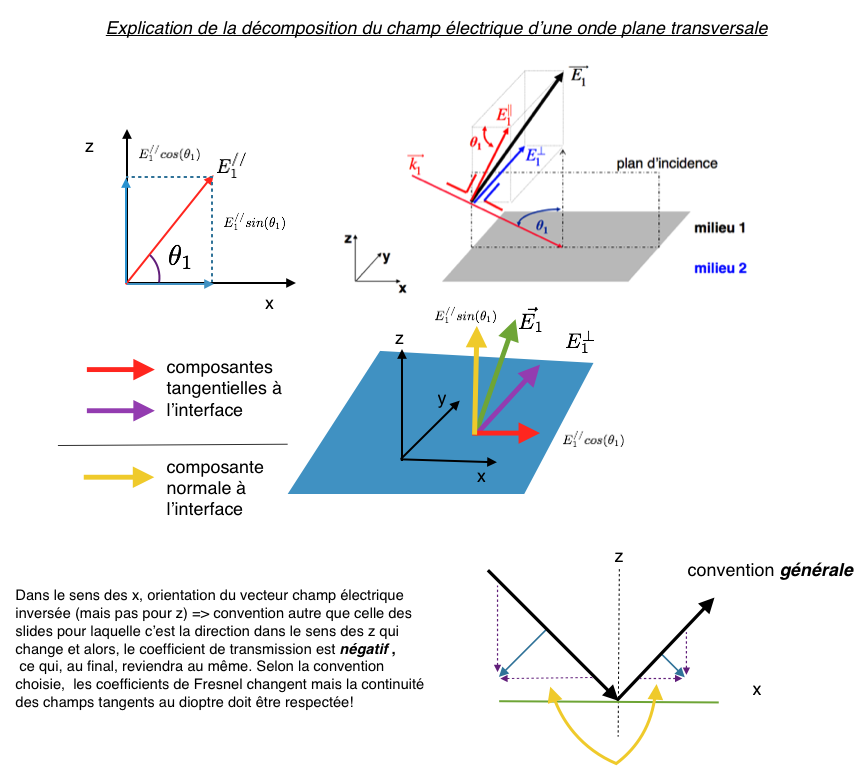
\includegraphics[height = 400pt,width = 450pt]{explicationbig.png}
%\end{center}


Nous écrivons sans peine en partant des composantes en $\hat{x}$ et des $\hat{y}$ les 4 conditions de continuité à l'interface du dioptre. Pour cela, il faut se rappeler le chapitre 1, dans lequel nous avons mentionné que les conditions limites aux interfaces imposaient que la partie tangentielle du champ E et du champ H soit conservée (en l'absence de charges et de courants à l'interface, ce qui est bien le cas ici). Nous devons donc imposer la continuité selon les axes $\hat{x}$ et $\hat{y}$. %\footnote{Claude dit NON: Nous adoptons la convention dénotée à la page précédente; celle du cours sera donnée juste après en titre de conclusion.} :  
\begin{equation*}
\begin{split}
\mbox{Continuité de $\vec{E}(\vec{r},t)$ selon $\hat{x}$ : }&\hspace{5pt} E^{\parallelsum}_{1i} \cos(\theta_{1}) +E^{\parallelsum}_{1r} \cos(\theta_{1}) = E^{\parallelsum}_{2t} \cos(\theta_{2})\\
\mbox{Continuité de $\vec{E}(\vec{r},t)$ selon $\hat{y}$ : }&\hspace{5pt} E_{1i}^{\perp} + E_{1r}^{\perp} = E_{2t}^{\perp}  \\
\mbox{Continuité de $\vec{H}(\vec{r},t)$ selon $\hat{x}$ : }&\hspace{5pt} Z_2E^{\perp}_{1i}\cos(\theta_{1}) - Z_2E^{\perp}_{1r} \cos(\theta_{1}) = Z_1E^{\perp}_{2t} \cos(\theta_{2})   \\
\mbox{Continuité de $\vec{H}(\vec{r},t)$ selon $\hat{y}$ : }&\hspace{5pt} Z_2E^{\parallelsum}_{1i} - Z_2E_{1r}^{\parallelsum} = -Z_1E_{2t}^{\parallelsum}
\end{split}
\end{equation*}
  
où $E_{1i}^{\parallelsum}$, $E_{1i}^{\perp}$, $\theta_{1}$,$\theta_{2}$, $Z_1$ et $Z_2$ sont connus. \\
Nous pouvons établir un système matriciel étant donné le caractère \textit{linéaire} des équations.
%\begin{fullwidth}
%\begin{center}
	$$
	\begin{pmatrix}
	-\cos \theta_{1} & 0 & \cos \theta_{2}& 0\\
	0 & -1 & 0 & 1\\
	0 & Z_2\cos \theta_{1} & 0 & Z_1\cos \theta_{2}\\ 
	Z_2 & 0 & -Z_1 & 0
	\end{pmatrix}
	\cdot
	\begin{pmatrix}
	E_{1r}^{\parallelsum}\\
	E_{1r}^{\perp}\\
	E_{2t}^{\parallelsum} \\ 
	E_{2t}^{\perp}
	\end{pmatrix}
	=
	\begin{pmatrix}
	E_{1i}^{\parallelsum} \cos \theta_{1}\\
	E_{1i}^{\perp} \\
	Z_2E_{1i}^{\perp} \cos \theta_{1} \\
	Z_2E_{1i}^{\parallelsum}
	\end{pmatrix}
	$$
%\end{center}
%\end{fullwidth}
%\vspace{10pt}
Nous pouvons résoudre ce système d'équations et obtenir les 4 coefficients de Fresnel suivants:
\[r_{\parallelsum} \overset{\Delta}= \frac{E_{1r}^{\parallelsum}}{E_{1i}^{\parallelsum}} = \frac{Z_{2}\cos \theta_{2} - Z_{1} \cos \theta_{1} }{Z_{2} \cos \theta_{2} + Z_{1} \cos \theta_{1} } \]
\[r_{\perp} \overset{\Delta}= \frac{E_{1r}^{\perp}}{E_{1i}^{\perp}} = \frac{Z_{2}\cos \theta_{1} - Z_{1} \cos \theta_{2} }{Z_{2} \cos \theta_{1} + Z_{1} \cos \theta_{2}}\]
\[t_{\parallelsum} \overset{\Delta}= \frac{E_{2t}^{\parallelsum}}{E_{1i}^{\parallelsum}} = \frac{2 Z_{2} \cos \theta_{1} }{Z_{2} \cos \theta_{2} + Z_{1} \cos \theta_{1}} \]
\[t_{\perp} \overset{\Delta}= \frac{E_{2t}^{\perp}}{E_{1i}^{\perp}} \frac{2 Z_{2} \cos \theta_{1} }{Z_{2} \cos \theta_{1} + Z_{1} \cos \theta_{2}}\]
Ces coefficients sont valables dans les milieux avec une permittivité électrique et une perméabilité magnétique constantes. La forme des équations de Fresnel ici présentes n'est pas unique. En effet, il existe des équations de Fresnel sous une forme plus restrictive. Cette forme n'utilise pas les impédances des deux milieux mais leur indice de réfraction. Elle est utilisée couramment chez des opticiens pour cette raison. L'inconvénient est que ladite forme n'est valable que pour des milieux dont la perméabilité magnétique est celle du vide (autrement dit, pour des matériaux non-magnétiques). Pour les opticiens, il ne s'agit pas d'un problème car la plupart des matériaux utilisés en optique sont non-magnétiques. Dans le cadre de ce cours, nous utiliserons toujours de préférence les formules énoncées plus haut. Néanmoins, voici les équations de Fresnel avec les indices de réfraction: 
\sidenote[][-5cm]{Afin de visualiser la réflexion et la réfraction au mieux,  il existe deux animations \textit{Matlab} très bien réalisées disponibles sur le site Moodle du cours.}% En prime\footnote{Disponible dans le fichier .zip}, un autre programme \textit{Matlab} vous permettant  de calculer rapidement les coefficients de \textit{Fresnel} suivant la convention du cours. Il est conseillé d'analyser la notice d'utilisation. \textbf{Notez} que si vous désirez afficher les graphes de l'évolution des coefficients de \textit{Fresnel} par rapport à l'angle incident; il vous faut simplement appeler la fonction avec le rapport $\frac{n_{1}}{n_{2}}$ souhaité entre les deux milieux. Enfin, ce programme est rapidement fait et n'est certainement pas optimisé ni défensif; il a pour but d'être le substitut à une calculette un peu longue à manier pour des calculs de \textit{coefficients de Fresnel}.}:  

\[r_{\parallelsum} \overset{\Delta}= \frac{E_{1r}^{\parallelsum}}{E_{1i}^{\parallelsum}} = \frac{n_{1}\cos \theta_{2} - n_{2} \cos \theta_{1} }{n_{2} \cos \theta_{1} + n_{1} \cos \theta_{2} } = \frac{\tan(\theta_{1}-\theta_{2})}{\tan(\theta_{1}+\theta_{2})}\]
\[r_{\perp} \overset{\Delta}= \frac{E_{1r}^{\perp}}{E_{1i}^{\perp}} = \frac{n_{1}\cos \theta_{1} - n_{2} \cos \theta_{2} }{n_{2} \cos \theta_{2} + n_{1} \cos \theta_{1}} = -\frac{\sin(\theta_{1} - \theta_{2})}{\sin(\theta_{1} + \theta_{2})} \]
\[t_{\parallelsum} \overset{\Delta}= \frac{E_{2t}^{\parallelsum}}{E_{1i}^{\parallelsum}} = \frac{2 n_{1} \cos \theta_{1} }{n_{2} \cos \theta_{1} + n_{1} \cos \theta_{2}} \]
\[t_{\perp} \overset{\Delta}= \frac{E_{2t}^{\perp}}{E_{1i}^{\perp}} \frac{2 n_{1} \cos \theta_{1} }{n_{2} \cos \theta_{2} + n_{1} \cos \theta_{1}}\]

%\subsection{Convention du cours: NON: il faut directeemnt utiliser la bonne convention, dit Claude}

%En ce qui concerne la convention du cours, il est seulement nécessaire de modifier le signe du coefficient $r_{//}$ ainsi que le signe des composantes en $\hat{x}$ et en $\hat{z}$ de tous les champs réfléchis et transmis dont nous parlions ci-dessus. 
Les deux formes des coefficients de Fresnel sont évidemment équivalentes si $\mu_1 = \mu_2 = \mu_0$. Il est aussi possible de rencontrer dans la littérature d'autres formes pour les équations de Fresnel, résultant d'une convention différente prise pour le sens dit positif des champs. 
%\todo{Analyser les graphes p21 et suivants dans CM4, + dire ce que veut dire le signe du coeff de Fresnel, car les champs etant alternatifs, le signe du coeff de Fresnel indique si les champs sont en phase tels que dessinés ou pas, et rien d'autre; si on change le sens des conventions, le signe du coeff change; mais ne pas oublier que les champs changent de sens toutes les demi-periodes ... }
\section{Conséquences des équations de Fresnel}
Supposons une interface entre deux milieux non-magnétiques (pour simplifier l'analyse), par exemple, une interface air-lucite (la lucite est le nom correct du plexiglas, qui est à la base une marque de produit).

Lorsqu'une onde EM passe de l'air vers la lucite, à incidence normale ($\theta_1=0^\circ$ sur la figure \ref{fig_ref2}), nous remarquons que les coefficients de réfraction sont négatifs. \textit{La réflexion change donc le sens du champ électrique} en lui appliquant un déphasage de $180^\circ$.\sidenote{Attention, il ne s'agit pas d'une histoire de conventions, le déphasage est bien réel. Pour s'en convaincre, il suffit de regarder les figures \ref{fig_convention1} et \ref{fig_convention2} en imaginant $\theta_1=0^\circ$. Nous pouvons remarquer que dans ce cas les vecteurs se confondent.} Avec une analyse similaire, on peut déterminer que la transmission ne change pas le sens du champ électrique.\\
Toujours dans le même cas (air $\rightarrow$ lucite), nous observons qu'à incidence rasante ($\theta_1$ proche de $90^\circ$), le coefficient de réfléxion tend vers 1 et le coefficient de transmission vers zéro. \textit{A incidence rasante, la réflexion est totale.}\\

Dans le cas inverse, visible à la figure \ref{fig_ref3}, où $n_1>n_2$ (lucite $\rightarrow$ air), nous pouvons observer que tant le champ électrique transmis que réfléchi est du même sens que le champ électrique incident. Une remarque importante s'impose quant à la définition du sens des champs. Ces champs sont des ondes sinusoïdales, dont l'orientation change toutes les demi-périodes. Par sens, on entend bien le sens pris au même moment, à l'interface. Autrement dit, si un coefficient de Fresnel est positif pour les sens définis aux figures \ref{fig_convention1} et \ref{fig_convention2}, cela signifie qu'à un moment fixé, au point de réflexion, les champs ont le sens tel qu'indiqué sur la figure. Une demi-période plus tard, les champs seront tous (en même temps) dans le sens opposé. 

\section{Angles particuliers}
\begin{marginfigure}%[-9cm]
	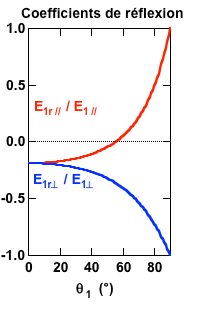
\includegraphics[width=\linewidth]{ref2}
	\caption{Coefficients de réflexion parallèle et perpendiculaire lorsque $n_1<n_2$ (air $\rightarrow$ lucite)}
	\label{fig_ref2}
\end{marginfigure} 
\begin{marginfigure}%[-9cm]
	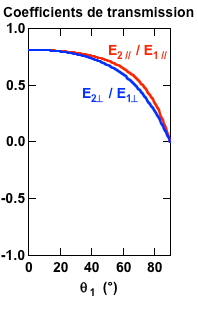
\includegraphics[width=\linewidth]{trans2}
	\caption{Coefficients de transmission parallèle et perpendiculaire lorsque $n_1<n_2$ (air $\rightarrow$ lucite)}
	\label{fig_trans2}
\end{marginfigure} 

\subsection{Angle de \textit{Brewster} et transmission totale}

Nous pouvons remarquer que le coefficient $r_{\parallelsum}$ peut s'annuler dans le cas particulier où $Z_2\cos\theta_{2} = Z_1\cos\theta_{1}$, autrement dit lorsque 
\[\sin^2\theta_1 = \frac{\mu_2\epsilon_1/\mu_1\epsilon_2 - 1}{(\epsilon_1/\epsilon_2)^2-1}\]

Pour des milieux non-magnétiques ($\mu_1 = \mu_2 = \mu_0$), cela revient à 
\[\sin\theta_1 = (\epsilon_1/\epsilon_2+1)^{-1/2}\]

Cet angle $\theta_1$ est appelé \textit{angle de Brewster} et se note $\theta_{B}$. \\

Nous pouvons également retrouver cet angle (pour des milieux non-magnétiques) à partir de l'expression optique du coefficient $r_{\parallelsum}$ : 
\[\frac{n_{2}\cos \theta_{1} - n_{1} \cos \theta_{2} }{n_{2} \cos \theta_{1} + n_{1} \cos \theta_{2} } = 0 \Leftrightarrow n_{2} \cos \theta_{1} = n_{1} \cos \theta_{2} \Rightarrow \cos^{2} \theta_{2} = \left(\frac{n_{2} \cos \theta}{n_{1}}\right)^{2}\]
En utilisant la loi de \textit{Snell-Descartes} : 
\[n_{1} \sin \theta_{1} = n_{2} \sin \theta_{2} \Rightarrow \sin^{2} \theta_{2} = \left(\frac{n_{1} \sin \theta}{n_{2}}\right)^{2} \] 
En se souvenant de l'identité trigonométrique de base $ \cos^{2} \alpha + \sin^{2} \alpha = 1$ : 
\[\sin^{2} \theta_{1} + \cos^{2} \theta_{1} = \left(\frac{n_{1} \sin \theta}{n_{2}}\right)^{2} +  \left(\frac{n_{2} \cos \theta}{n_{1}}\right)^{2}\]
\[\sin^{2} \theta_{1} \left(\frac{n_{2}^{2} - n_{1}^{2}}{n_{2}^{2}}\right) = \cos^{2} \theta_{1} \left(\frac{n_{2}^{2} - n_{1}^{2}}{n_{1}^{2}}\right)\]
Enfin, nous pouvons écrire : 
\[\tan^{2} \theta_{1} = \frac{n_{2}^{2}}{n_{1}^{2}} \Rightarrow \theta_{1} \overset{\Delta}= \theta_{B} = \arctan\left(\frac{n_{2}}{n_{1}}\right)\]

De la même manière, on peut calculer l'angle pour lequel $r_{\perp}$ s'annule. On montre facilement que dans ce cas, un angle de Brewster n'existe que si les milieux sont magnétiques. Pour des milieux non-magnétiques, il n'y a jamais de transmission totale lorsque l'onde est polarisée perpendiculairement au plan d'incidence. 

Ces principes sont à la base du fonctionnement des polariseurs, c'est-a-dire des dispositifs produisant de la lumière polarisée. Si un rayonnement électromagnétique comportant une égale quantité des deux polarisations rencontre une interface entre deux milieux non-magnétiques sous un angle égal à l'angle de Brewster, la transmission sera totale pour la fraction de l'onde polarisée parallèlement au plan d'incidence, et partielle pour l'autre. On a donc polarisé l'onde transmise, en modifiant sa polarisation. De manière tout à fait générale, \textbf{l'état de polarisation} d'une onde change suite à une réfraction ou une réflexion en ce sens où l'amplitude des différentes composantes polarisées a été modifiée par les coefficients de \textit{Fresnel}. 

%\begin{center}
%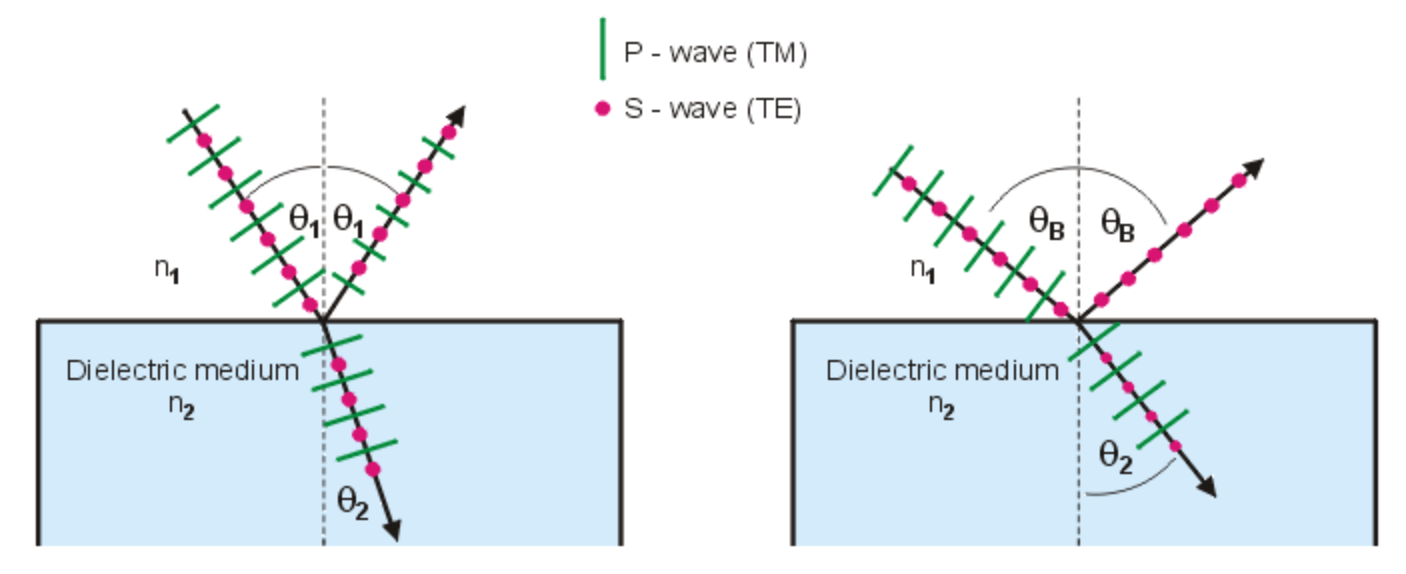
\includegraphics[height = 175pt, width = 300pt]{brewster.png}
%\end{center}

\subsection{Angle critique et réflexion totale}
\begin{marginfigure}%[-9cm]
	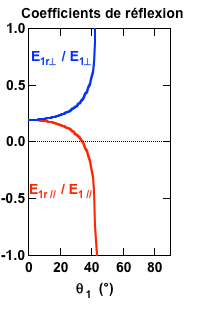
\includegraphics[width=\linewidth]{ref1}
	\caption{Coefficients de réflexion parallèle et perpendiculaire lorsque $n_1>n_2$ (lucite $\rightarrow$ air)}
	\label{fig_ref3}
\end{marginfigure} 
\begin{marginfigure}%[-9cm]
	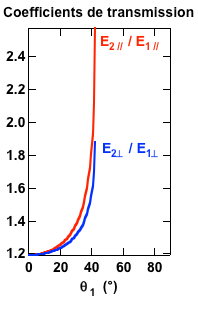
\includegraphics[width=\linewidth]{trans1}
	\caption{Coefficients de transmission parallèle et perpendiculaire lorsque $n_1>n_2$ (lucite $\rightarrow$ air)}
\end{marginfigure} 
Lorsque le milieu où s'opère la \textit{transmission} admet un indice de réfraction $n_{2}<n_{1}$, il existe un \textit{angle critique} d'incidence à partir duquel la réflexion est \textit{\textbf{totale}}, c'est-à-dire un angle au-delà duquel l'angle $\theta_2$ devient complexe et n'existe donc pas (pour un angle d'incidence égal à cet angle critique, $r_{\parallelsum}$ et $r_{\perp}$ sont égaux à  -1 et 1 respectivement; au delà de cet angle critique, les coefficients de Fresnel ne sont évidemment pas définis). 

Il faut noter que ce phénomène intervient quelle que soit la polarisation de l'onde incidente, pour des milieux magnétiques ou non, mais n'est possible qu'en passant d'un milieu plus réfringent à un milieu moins réfringent ($n_{2} < n_1$), par exemple, de la lucite (ou de l'eau, ...) vers l'air.\\ 

Par l'approche des coefficients de \textit{Fresnel}, nous remarquons tout de suite que \textit{l'angle critique} est l'angle d'incidence $\theta_{1} = \theta_{c}$ pour lequel l'angle de réfraction vaut $\frac{\pi}{2}$, ce qui nous donne: 
\[\sin \theta_{c} = \frac{n_{2}}{n_{1}} \Rightarrow \theta_{c} = \arcsin \frac{n_{2}}{n_{1}}\]
\begin{marginfigure}%[-3cm]
	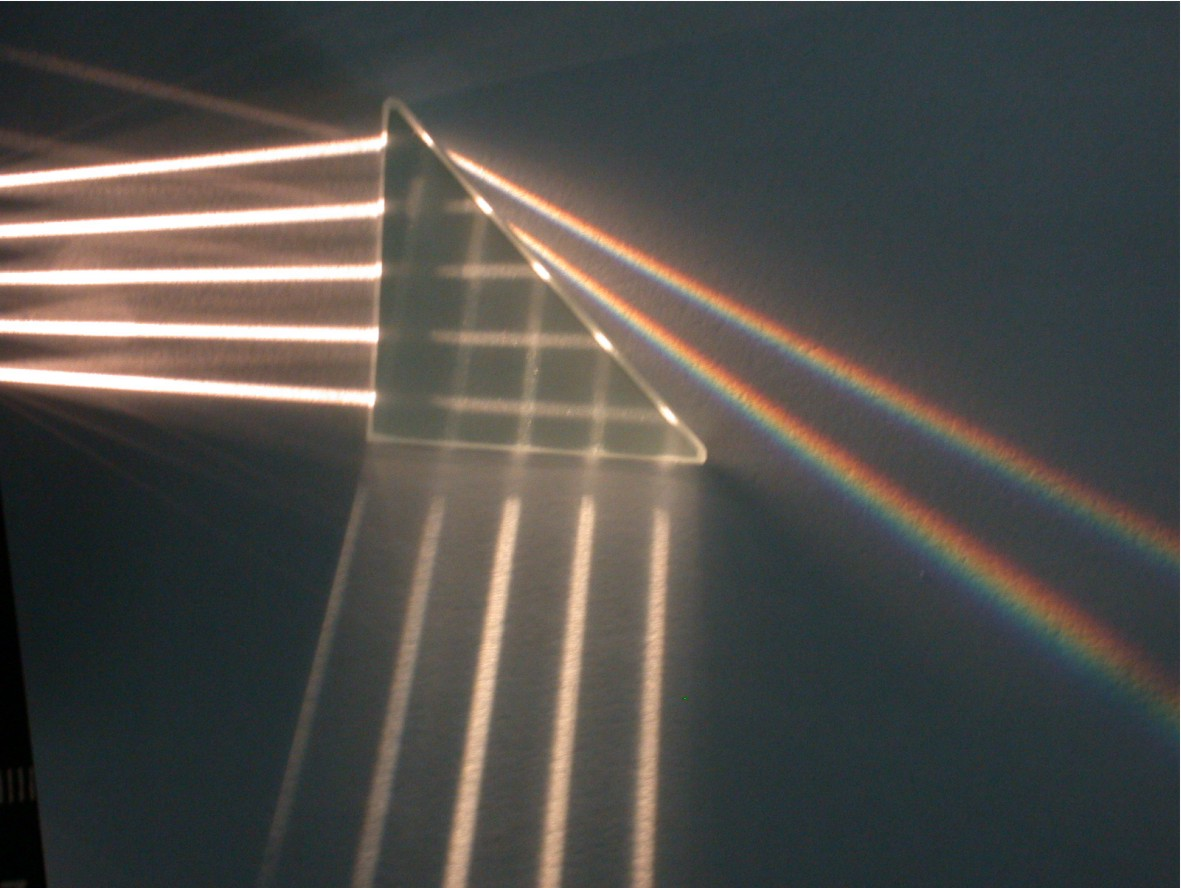
\includegraphics[width=\linewidth]{reflexion_tot}
	\caption{Illustration de la réflexion totale, les deux premières raies incidentes en partant du haut sont en dessous de l'angle critique, une partie de l'onde est donc transmise. A partir de la 3ème raie, plus aucune onde n'est transmise}
\end{marginfigure}
%\todo{De manière générale : Découper les schémas et les stacker verticalement pour utiliser l'espace sur la droite (marginfigure); refaire le schéma avec les conventions du cours ; importer le schéma des conventions slide p16; parler histoire?}

	\chapter{Interférences}
Les interférences sont des phénomènes apparaissant aux points de l'espace où se propagent des ondes générées par des sources différentes. Puisque les effets \footnote{champs électromagnétiques, déplacements,...} en provenance de ces sources s'additionnent vectoriellement en tout point, des effets d'interférence constructive ou destructive sont possibles. L'intensité résultante n'est donc a priori pas égale à la somme des intensités de chaque onde. 

Ces effets sont très importants dans la caractérisation des phénomènes ondulatoires. Dans l'histoire des sciences, ils ont entre autres permis de prouver qu'un phénomène est bien ondulatoire. La preuve que la lumière ne possède pas uniquement un aspect corpusculaire\footnote{théorie initiale élaborée entre autres par Newton} a été apportée par ce principe (voir \textit{expérience de Young}).

Dans la grande majorité des cas, lorsque l'on est en présence de plusieurs ondes de sources différentes, le principe de superposition s'applique simplement en additionnant (vectoriellement) les grandeurs des deux ondes. L'ensemble des relations établies dans ce chapitre se basent sur ce principe. Pour être complet, il faut cependant noter que dans certaines situations, des conditions aux limites doivent être prises en compte et peuvent compliquer le raisonnement. Par exemple, supposons que 2 personnes secouent une corde verticalement à ses deux extrémités. Il faut décomposer le déplacement de la corde en 2 et appliquer le principe de superposition pour connaître le déplacement total. Pour le sous-problème de l'onde générée par la personne de gauche, la condition limite impose que le déplacement soit nul à l'extrémité droite. Réciproquement, le deuxième sous-problème possède une condition limite imposant un déplacement nul à l'extrémité gauche de la corde. La combinaison de ces conditions avec le principe de superposition permettent donc à la corde de respecter les déplacements imposés à ses deux extrémités.

\section{Interférence entre deux sources de même fréquence}

\begin{marginfigure}[0cm]
	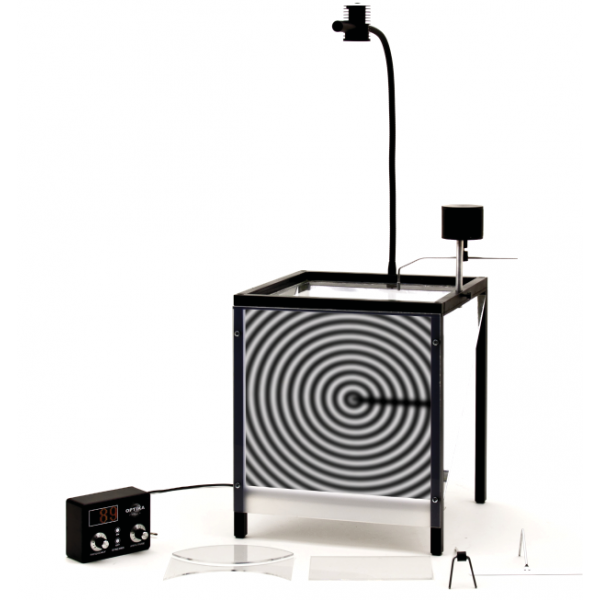
\includegraphics[width=5cm]{cuves-a-ondes}
	\caption{Cuve à ondes}
\end{marginfigure}

L'observation de ce phénomène peut être réalisée sur une cuve à ondes. Celle-ci contient un bac rempli d'eau et surmonté par deux pointes en mouvement vertical sinusoïdal. Deux ondes circulaires sont alors générées par la vibration des pointes qui affleurent l'eau.

Lorsque les pointes oscillent exactement en phase, les deux sources ponctuelles sont dites cohérentes. Pour simplifier les calculs, nous négligeons l'atténuation de leur amplitude avec la distance. Comme indiqué ci-dessus, nous travaillons dans l'hypothèse du principe de superposition, c'est-à-dire que l' onde résultante est la simple somme du déplacement vertical des deux ondes émises par les sources. Ce principe est une bonne approximation, tant que les amplitudes des deux ondes sont faibles. Si les amplitudes deviennent importantes, des non-linéarités apparaissent, mais elles ne seront pas abordées dans ce cours. 

\begin{figure}[htb]
\centering
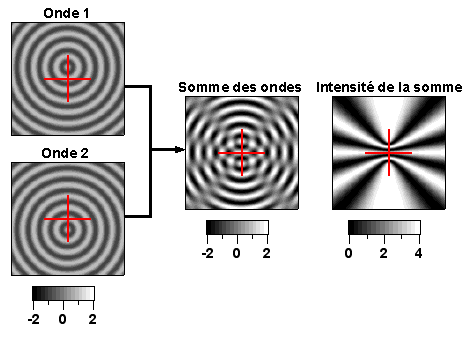
\includegraphics[scale=0.5]{omega}
\caption{Intensité résultante de deux sources ponctuelles}
\label{omega}
\end{figure}

Sur la figure \ref{omega} dont l'animation est disponible sur le site web\footnote{\url{http://perso.uclouvain.be/alain.jonas/Cours/FSAB1203/}}, la somme des deux ondes présente des bandes grises fixes correspondant à une amplitude nulle\footnote{les niveaux de gris sont donnés par les barres sous chaque image}. Dans ces régions, appelées \textit{nodales} où se situent les \textit{noeuds}, l'oscillation est nulle à tous les instants; les deux ondes émises par les sources y interfèrent de manière destructive. Cela se produit quand les maxima des oscillations (les bosses) de la première onde coïncident avec les minima des oscillations (les creux) de la seconde. Entre ces régions, on trouve un comportement ondulatoire typique.

Le graphe de droite représente l'intensité de l'onde résultante qui, pour rappel, représente aussi le flux d'énergie véhiculé localement par l'onde en $W/m^2$, moyenné sur une durée beaucoup plus grande que la période. Contrairement aux trois autres graphes, cette image est fixe, puisqu'il s'agit d'une moyenne sur le temps. Le graphe du milieu lui est semblable car l'intensité est proportionnelle au carré de l'amplitude du déplacement vertical de l'onde, et les bandes d'amplitude nulles correspondent bien aux lignes d'intensités nulles de la figure de droite. Par contre, l'intensité est forte à d'autres endroits, là où les deux ondes primaires interfèrent constructivement: il s'agit des régions \textit{anti-nodales} où se situent les \textit{ventres}, dans lesquelles les maxima de la première onde coïncident avec les maxima de la seconde.
 
Analysons tout d'abord le comportement de l'onde résultante sous forme graphique. La figure \ref{point} analyse la valeur de l'amplitude des ondelettes en 3 points à la surface de l'eau.

\begin{figure}[htb]
\centering
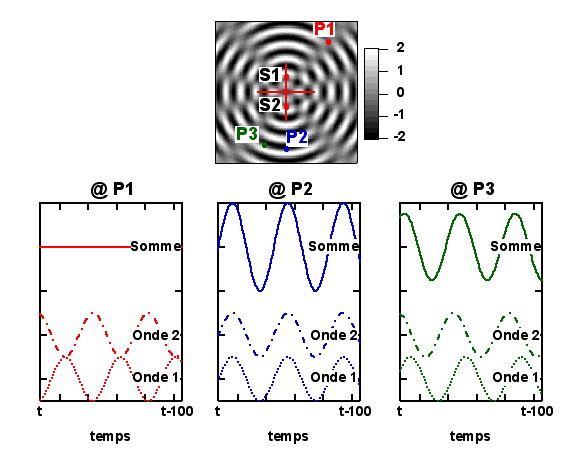
\includegraphics[scale=0.7]{point}
\caption{Analyse des ondulations en différents points à la surface de l'eau}
\label{point}
\end{figure}

L'onde émise en $S_1$ prend moins de temps à atteindre le point rouge ($P_1$) que l'onde émise en $S_2$. Le retard de l'une par rapport à l'autre est tel que les maxima de l'une correspondent aux minima de l'autre, et la résultante est nulle (fig. @P1) : l'interférence est destructive. En $P_2$ par contre, le retard de la première onde par rapport à la seconde est tel que les maxima (et les minima) des deux ondes coïncident. Les ondes interfèrent de manière constructive, et l'amplitude de l'onde résultante est double de celle de chacune des ondes primaires. Enfin, en $P_3$, la situation est intermédiaire.

Passons à une description mathématique de ces interférences dans laquelle nous écrivons le champ total en un point $P$ quelconque de l'espace. Les relations ci-dessous conviennent pour le cas simplifié de deux sources ponctuelles cohérentes, de même amplitude, de même longueur d'onde\footnote{dans la cuve à ondes, c'est trivial puisque les ondes se propagent dans le même milieu} et de même polarisation\footnote{dans la cuve à ondes, la polarisation n'a pas de sens puisque la grandeur analysée est scalaire: le déplacement vertical}. Nous considérerons également que les ondes primaires sont des ondes circulaires, polarisées dans la direction de l'axe des $z$ et de forme sinusoïdale.
Le champ créé en $P$ par la première onde est de la forme 
$$A \cos (kr_1-\omega t)\overset\rightarrow{\mbox{l}_z},$$
où $r_1$ est la distance entre la première source et le point $P$, et $k=2\pi/\lambda$ est le nombre d'onde. 

De la même manière, le champ créé en $P$ par la seconde onde est de la forme 
$$A \cos (kr_2-\omega t +\phi_2)\overset\rightarrow{\mbox{l}_z},$$
où $r_2$ est la distance entre la seconde source et le point $P$, et $\phi_2$ est un terme prenant en compte un éventuel déphasage entre les deux sources. 

En $P$, le champ résultant total est donc:

\begin{align*}
\overset\rightarrow{E}(P)&=A \cos (kr_1-\omega t)\overset\rightarrow{\mbox{l}_z} + A \cos (kr_2-\omega t +\phi_2)\:\overset\rightarrow{\mbox{l}_z} \\&
=A \bigg(\cos (kr_1-\omega t)+ \cos (kr_2-\omega t +\phi_2)\bigg)\:\overset\rightarrow{\mbox{l}_z}\\&
=A \bigg(2\cos \Big(\frac{\phi_2 +kr_2-kr_1}{2}\Big)\cos \Big(\frac{\phi_2 +kr_2+kr_1}{2}-\omega t\Big)\bigg)\:\overset\rightarrow{\mbox{l}_z}\\&
=\underbrace{2A\cos \Big(\frac{\phi}{2}\Big)}_\textrm{amplitude}\underbrace{\cos (\phi'-\omega t)}_\textrm{oscillation}\:\overset\rightarrow{\mbox{l}_z}
\end{align*}

où $\phi=\phi_2 +kr_2-kr_1$ et $\phi'=(\phi_2 +kr_2+kr_1)/2$.

Cette fonction possède une partie liée à l'amplitude qui est modulée spatialement par $\cos (\phi/2)$. Ce terme est indépendant du temps et ne dépend donc que de la position du point $P$. La figure d'interférence\footnote{
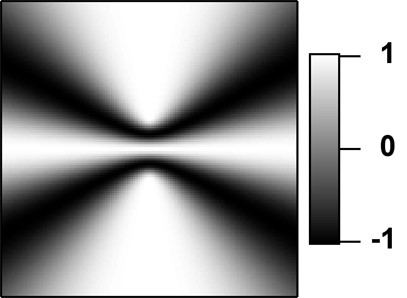
\includegraphics[scale=0.63]{M6}} des deux sources est établie dès la création des premières oscillations.
Le lieu des points de même amplitude est une hyperbole dont les foyers sont les deux sources initiales puisqu'il satisfait
$$2A\cos \Big(\frac{\phi_2 +k(r_2-r_1)}{2}\Big)=Constante.$$
C'est bien l'équation d'une hyperbole, c'est-à-dire l'ensemble des points dont la différence des distantes $r_2-r_1$ est constante.

L'onde se déplace suivant des ellipses\footnote{
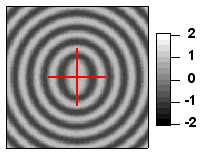
\includegraphics[scale=0.6]{M5}}. En effet, nous cherchons le lieu des points de même déplacement vertical à tout moment, c'est-à-dire les points dont l'argument du cosinus\footnote{partie de $y(P)$ liée au temps} est identique.
En particulier pour $t=0$, le lieu des point devient
$$\phi'=\frac{\phi_2 +kr_2+kr_1}{2}=Constante$$ 
et décrit bien une ellipse, l'ensemble des points dont la somme des distances $r_1+r_2$ est constante.
Nous obtenons ensuite une expression pour l'intensité, qui est proportionnelle au carré de l'amplitude:
$$I\propto 4A^2\cos^2 \Big(\frac{\phi}{2}\Big)$$
L'onde résultante en $P$ s'exprime donc comme le produit d'une fonction oscillante qui traduit le caractère ondulatoire de l'onde résultante, et d'une amplitude généralisée. Cette amplitude généralisée fait apparaître $\phi$, qui est le déphasage entre la seconde et la première onde au point P, c'est-à-dire la différence entre la phase de l'onde 2 en P et la phase de l'onde 1 en P. Ces phases résultent de la propagation des ondes sur des distances données (les termes en $kr_i$), et des phases des sources elles-mêmes ($\phi_2$). Le déphasage est une fonction de l'espace, mais pas du temps.

\fbox{\begin{minipage}{1.5\textwidth}
   Lorsque le déphasage vaut un multiple impair de $\pi$,
   \begin{itemize}
   \item $\phi=(2n+1)\pi$ et $\cos(\phi/2)=0$: les ondes interfèrent de manière destructive. C'est le cas en $P_2$.
   \end{itemize}
Si par contre le déphasage vaut un multiple pair de $\pi$, 
\begin{itemize}
   \item $\phi=2n\pi$ et $\cos(\phi/2)=\pm 1$: les ondes interfèrent de manière constructive. C'est le cas en $P_1$.
   \end{itemize}
   
L'intensité
\begin{itemize}
   \item est nulle pour les points auxquels les ondes interfèrent de manière destructive;
   \end{itemize}
          \begin{itemize}
   \item est proportionnelle à $4A^2$ là où les ondes interfèrent de manière constructive
   \end{itemize}

\end{minipage}}

L'intensité dans ces régions vaut 4 fois celle de chacune des ondes primaires, soit deux fois plus que la somme des intensités des ondes primaires. L'énergie n'est par pour autant créée, les interférences provoquent une redistribution spatiale de l'énergie: certains endroits sont appauvris (interférences destructives), d'autres sont enrichis (interférences constructives), et l'intégrale sur toute la surface est constante, et vaut la somme des intensités émises par chaque source primaire.

\begin{marginfigure}[6cm]
	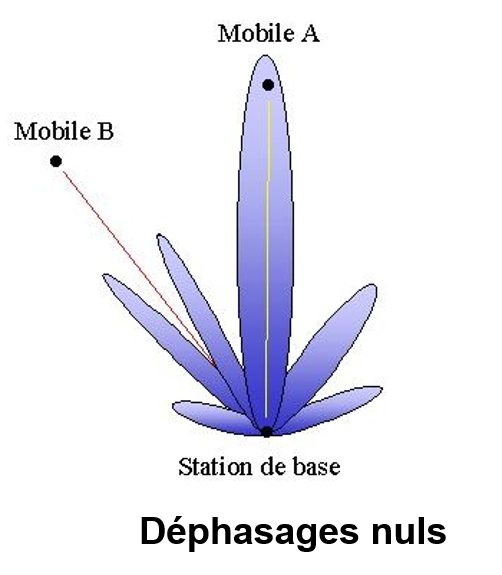
\includegraphics[scale=0.5]{M7}
	\caption{Diagramme polaire}
	\label{fm7}
\end{marginfigure}

Cette redistribution d'énergie permet de diriger l'onde dans une direction préférentielle. Un premier exemple d'application de ce principe sont les casques anti-bruits qui atténuent fortement l'ensemble des bruits extérieurs. Ils possèdent un micro qui analyse le bruit extérieur et qui crée une source qui compense le bruit externe dans la direction du tympan de l'oreille. Une autre application de ce principe se retrouve dans le domaine des télécommunications. En transmission satellite, et plus récemment dans les standards de transmission Wi-fi et 4G, plusieurs antennes sont utilisées conjointement pour choisir des directions préférentielles dans lesquelles on transmet l'information avec une plus grande puissance. Pour ces groupes d'antennes (ou pour les antennes directives telles que les antennes paraboliques), on définit généralement un diagramme de rayonnement (fig \ref{fm7}) qui représente l'intensité qui est envoyée en fonction de la direction. En d'autres termes, la longueur de l'ellipse reflète l'intensité émise ou perçue\footnote{Grâce au principe de réciprocité valable en électromagnétisme, ce diagramme de rayonnement est toujours le même, pour une antenne ou un groupe d'antenne donné, en émission et en réception.} dans cette direction.   Un déphasage\footnote{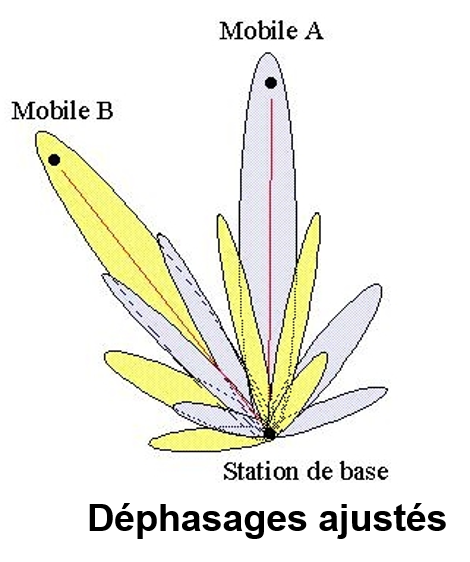
\includegraphics[scale=0.51]{M8}} entre les sources permet alors d'ajuster la direction d'intensité maximale de rayonnement. L'augmentation du nombre d'antennes permet une direction de plus en plus ciblée.
Les systèmes de radioastronomie utilisent aussi depuis longtemps ce procédé pour capter de l'information dans des directions spécifiques en provenance de très longues distances. Des réseaux d'antennes paraboliques sont couramment utilisés.

Revenons à notre problème à deux sources. Si les deux sources sont en phase ($\phi_2=0$), le déphasage en $P$ s'écrit $\phi=2\pi(r_2-r_1)/\lambda$, ce qui permet d'écrire les conditions encadrées ci-dessus de la façon suivante:

\fbox{\begin{minipage}{0.9\textwidth}
   Si les deux sources émettent en phase,
   \begin{itemize}
   \item lorsque la différence de chemin $(r2-r1)$ vaut un multiple impair de $\lambda/2$, 
   $$(r2-r1) = (n + 1/2)\lambda,$$ les ondes interfèrent de manière destructive.
             Les maxima de l'une se superposent aux minima de l'autre. 
   \item lorsque la différence de chemin $(r2-r1)$ vaut un multiple pair de $\lambda/2$
   $$(r2-r1) = n\lambda,$$ les ondes interfèrent de manière constructive.
            Les maxima de l'une se superposent aux maxima de l'autre.
   \end{itemize}

\end{minipage}}

Dans un grand nombre de cas, on ne s'intéresse pas en détail à l'intensité résultant de l'interférence entre deux sources (ou plus). Ce qui est recherché, c'est le lieu des points où l'intensité est maximale ou minimale, ou encore la longueur d'onde pour laquelle l'intensité est maximale ou minimale à un endroit donné, ou le déphasage à introduire entre deux sources pour avoir une intensité maximale ou minimale en un point donné de l'espace,...

Dans tous ces cas, le problème est réduit et consiste à déterminer les positions et phases des sources, et de calculer la distance entre ces sources et les points considérés. A partir de cela, on détermine le déphasage total, et on applique les règles des encadrés précédents. Examinons deux exemples ci-dessous.

Il convient d'énoncer tout d'abord le principe de Huygens sur lequel nous nous appuyons durant les prochains paragraphes:
\begin{center}
\textit{Chaque point atteint par une onde se comporte comme une source secondaire qui émet des ondelettes sphériques dans toutes les directions.}
\end{center}

\begin{figure}[htb]
\centering
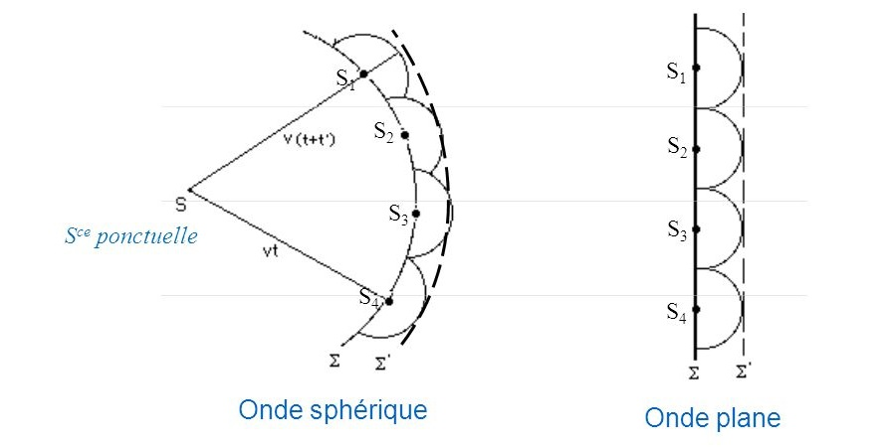
\includegraphics[scale=0.4]{M9.png}
\caption{Principe de Huygens}
\end{figure}

La propagation d'une onde circulaire revient alors à considérer la résultante de toutes les ondelettes circulaires générées à l'instant précédent.
Cet énoncé permet de prédire la position des fronts d’onde un instant plus tard ainsi que de calculer les effets d’interférences et de diffractions de façon suffisamment précise dans des cas simples.
Néanmoins, il est important de mentionner que ce principe est une {\it approximation} pour plusieurs raisons. Premièrement, ce sont en réalité des demi-cercles qui sont formés puisque l'onde résultante ne revient pas en arrière. Et deuxièmement, en pratique, la propagation des ondelettes sphériques ne se fait pas de manière équitable dans toutes les directions. Ce principe a par la suite été ajusté\footnote{au moyen de coefficients ajoutés dans les formules en fonction de la direction de propagation} par Fresnel et Kirchhoff, mais cela sort du cadre de ce cours.

Le problème auquel on s'intéresse est celui d'un écran percé de deux fentes infiniment étroites séparées par la distance $d$, illuminé par une onde plane arrivant avec une certaine incidence oblique (fig. \ref{3}). Une vague rencontrant une plaque percée par deux fentes de largeur infinitésimale correspond à ce problème.

\begin{figure}[htb]
\centering
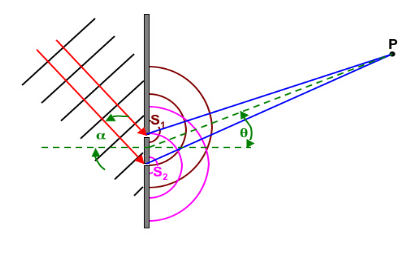
\includegraphics[scale=0.9]{3}
\caption{Interférence entre deux sources cohérentes, crées par l'illumination de deux fentes.}
\label{3}
\end{figure}

Dans ce dessin, les lignes rouges et les lignes bleues n'ont pas d'existence physique réelle. Elles correspondent à des «rayons», qui sont des droites perpendiculaires aux fronts d'onde. Les lignes noires, roses et brunes sont des lignes d'égale phase, par exemple des lignes correspondant aux endroits où le champ est maximal. Ces lignes avancent à la vitesse\footnote{dans le vide; sinon, il faut diviser $c$ par l'indice de réfraction} $c$. Par le principe de Huygens, l'onde plane arrivant vers la plaque se comporte comme deux sources d'ondes se propageant à droite de la plaque. Cette technique est utilisée entre autres pour obtenir deux sources d'ondes exactement à la même fréquence (sources cohérentes) car les ondes sont issues du même front d'onde. Obtenir la même fréquence dans un appareil n'est pas une chose aisée et une différence infime de fréquence peut parfois engendrer des résultats conséquents.

Si le point $P$ est situé très loin de l'écran, alors les lignes bleues connectant chacune des fentes au point P sont presque parallèles. 

L'\textit{approximation de Fraunhofer} consiste à considérer que ces droites sont réellement parallèles, une approximation que nous accepterons dans presque tous les exercices de ce cours.

Le déphasage d'une onde à un endroit donné, par rapport à la source, peut s'exprimer facilement en fonction de sa position. Nous le démontrons formellement dans le cas unidimensionnel d'une onde progressive se déplaçant vers la gauche
$$\xi(x,t)=\xi_1\sin(\omega t+kx).$$
En $x=d$, l'onde a pour équation 
$$ \xi(d,t)=\xi_1\sin(\omega t+kd).$$ 
Puisqu'en $x=0$, l'onde vaut 
$$ \xi(0,t)=\xi_1\sin(\omega t),$$ 
l'onde se déphase de $\Delta \phi=kd$ en parcourant une distance $d$. Nous pouvons dès lors en déduire la relation:
$$\Delta\phi=kd\Rightarrow\frac{\Delta\phi}{2\pi}=\frac{d}{\lambda}$$ 


Il est évident qu'il y a deux sources dans le problème, $S_1$ et $S_2$, correspondant aux sources des ondes émises par les fentes lorsqu'elles sont illuminées par l'onde plane. Ces deux sources n'émettent pas en phase, parce que l'onde plane arrive en $S_2$ un peu plus tard qu'en $S_1$. 
Calculons ce retard de phase entre les deux sources.

La distance supplémentaire\footnote{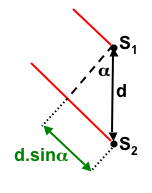
\includegraphics[scale=1]{7}} $d'$ parcourue par l'onde plane pour atteindre $S_2$ vaut $d\sin\alpha$. Compte-tenu du fait qu'une distance d'une longueur d'onde correspond à un déphasage de $2\pi$, le retard de phase de S2 par rapport à S1 est de 
$$ \phi_2=\frac{2\pi}{\lambda}d\sin\alpha.$$ 
Notons que la longueur d'onde dépend du milieu de propagation et ne correspond pas toujours à $c/f$.

Calculons à présent la différence de chemin\footnote{
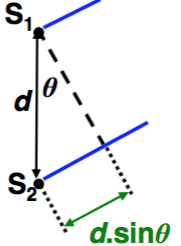
\includegraphics[scale=1]{2}} entre le point $P$ d'observation et les deux sources. Par l'approximation de Fraunhofer, elle ne dépend que de l'angle, et pas des coordonnées détaillées du point $P$: $r_2-r_1=d\sin\theta$.
Le déphasage résultant de cette différence de chemin vaut 
$$k(r_2-r_1)=\frac{2\pi}{\lambda}d\sin\theta.$$ 
Nous retrouvons une expression analogue à la précédente.

Il ne reste plus qu'à sommer ces deux termes pour obtenir le déphasage total, en faisant attention à prendre les bons signes pour les déphasages. Ici, $S_2$ est atteint plus tard par l'onde incidente, et le rayon émis par $S_2$ doit parcourir un chemin plus long pour atteindre $P$ que celui émis par $S_1$. Donc, il faut additionner les déphasages à l'incidence et à l'émission. La différence de phase totale est donc 
$$\phi=\frac{2\pi d}{\lambda}(\sin \theta +\sin \alpha).$$
Si cette différence vaut un multiple pair de $\pi$, l'interférence en $P$ est constructive; si elle vaut un multiple impair de $\pi$, l'interférence en $P$ est destructive. A partir de ces conditions, on peut dériver des conditions sur les angles ou la longueur d'onde de telle sorte que l'intensité soit nulle ou maximale à un endroit donné de l'espace. Par exemple, si on cherche les angles pour lesquels il y a interférence constructive avec $\alpha=0$ (incidence normale), on trouve: 
$$ \frac{2\pi d}{\lambda}\sin \theta=2m\pi$$
$$ \Rightarrow d \sin \theta =m\lambda$$
 où $m$ est un nombre entier, positif ou négatif. 
 
 Si nous plaçons un écran derrière les deux fentes, nous verrons une succession de bandes claires\footnote{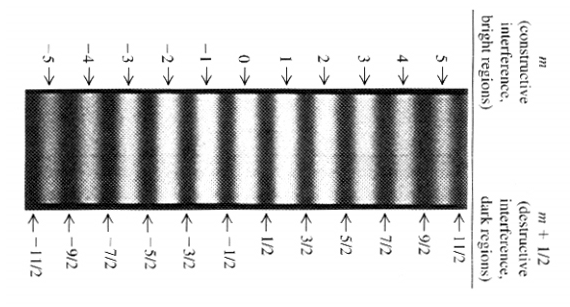
\includegraphics[scale=0.3]{8} Il s'agit ici du cas où les deux fentes sont des minces fentes verticales, les deux sources cohérentes sont dès lors approximativement cylindriques.} appelées franges d'interférence, chaque frange correspondant à une valeur entière de $m$. Cette expérience a été réalisée pour la première fois par Thomas Young\footnote{Médecin anglais, savant polyvalent (archéologue, philologue, physicien des matériaux [le module de Young],…).
 Il lit à 2 ans, et parle 10 langues à 16 ans (dont le Chaldéen, le Syriaque, le Turc et le Perse).} en 1801. Ce scientifique est le premier Anglais à contester la vision corpusculaire de Newton grâce à de multiples expériences sur les phénomènes d'interférences. Il a entre autres expliqué les anneaux de Newton\footnote{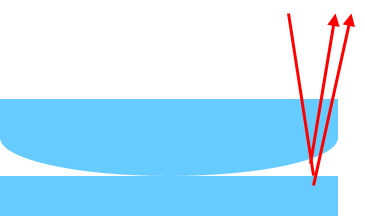
\includegraphics[scale=0.7]{M10} Un anneau de Newton désigne la figure d'interférence obtenue en plaçant une lentille sur une surface plane (voir section suivante).}, ainsi que la couleur des bulles de savon, et le phénomène d'interférence (deux ou plusieurs fentes), à partir d'une théorie ondulatoire. Ses découvertes n'ont pas été acceptée par la plupart des scientifiques car la théorie de Newton semblait décrire parfaitement la physique du monde et ne pouvait donc pas être remise en question.
 

% Les particules adoptent une distribution d’ensemble corrélée mais elles s’ignorent entièrement. En effet, la figure d'interférence\footnote{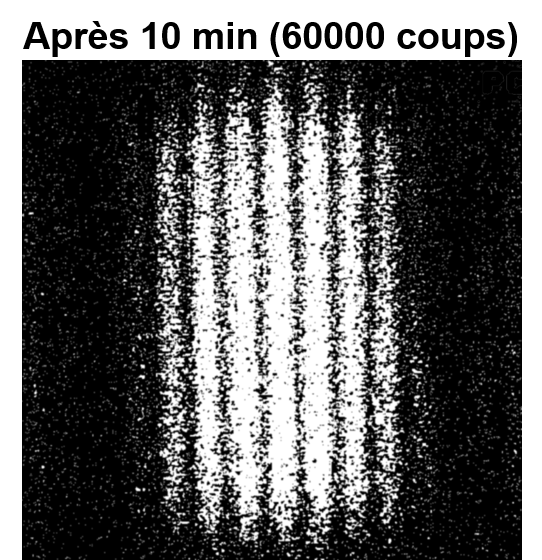
\includegraphics[scale=0.3]{M11} \\Évènements discrets: arrivée de photons (particules) selon une distribution de probabilité donnée par l'intensité du champ (onde).} issue d'une faisceau de particules apparaît aussi lorsque les particules sont envoyées l'une après l'autre. Dans ces conditions, il faut soit que les photons se comportent comme une onde, ou alors qu’ils obéissent de manière aléatoire à une loi statistique décrite par les formules d’interférence.


\section{Film illuminé par une onde plane}
\label{film_onde_plane}

Le second problème est le suivant: un film mince déposé sur un support plan est illuminé par une onde plane sinusoïdale. Cette onde plane rencontre plusieurs interfaces\footnote{par exemple les surfaces d'un polymère multicouche}, en se réfractant et se réfléchissant partiellement à chaque interface. Chaque faisceau réfracté et réfléchi peut lui-même rencontrer plusieurs interfaces, et se réfléchir ou se réfracter partiellement. On aboutit à une multitude d'ondes superposées, et donc à des interférences, comme illustré schématiquement sur la figure \ref{fig:film_mince}.

\begin{figure}[htb]
\centering
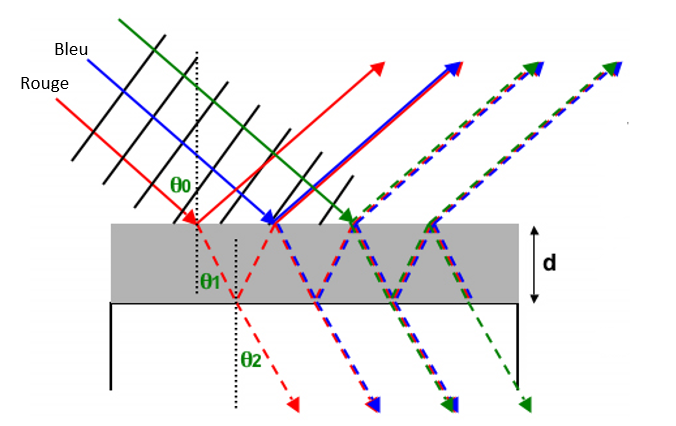
\includegraphics[scale=0.6]{9}
\caption{Interférences issues d'un film mince}
\label{fig:film_mince}
\end{figure}

Les longueurs d'ondes associées à chaque milieu sont données par:
\begin{itemize}
    \item Milieu supérieur $0$ ($n=n_0$): $\lambda_0=\lambda/n_0$
    \item Milieu moyen $1$ ($n=n_1$): $\lambda_1=\lambda/n_1$
    \item Milieu inférieur $2$ ($n=n_2$): $\lambda_2=\lambda/n_2$
\end{itemize}
où $\lambda$ correspond à la longueur d'onde dans le vide.

La loi de Snell permet d'écrire la relation
$$ n_0\sin \theta_0=n_1\sin \theta_1=n_2\sin \theta_2.$$

Dans la figure \ref{fig:film_mince}, trois rayons particuliers appartenant à l'onde sont tracés \sidenote[][-2cm]{il en existe une infinité, mais la situation se reproduit avec la même géométrie pour chacun des autres rayons pris deux à deux}. Les lignes noires sont les lignes de crête \sidenote[][0cm]{elles ne sont pas représentées pour les ondes réfléchies et réfractées, pour ne pas encombrer le dessin}. Concentrons-nous sur deux rayons, le rouge et le bleu, et à leurs deux réflexions qui interfèrent en émergeant du film. 

Pour atteindre le film, le rayon bleu parcourt une distance $a$ supplémentaire par rapport au rayon rouge. Par contre, le faisceau rouge (qui est réfracté, réfléchi puis de nouveau réfracté) atteindra le même point d'émergence que le premier faisceau réfléchi bleu, après avoir effectué un zig-zag\footnote{
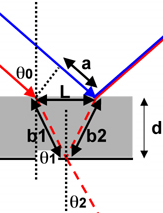
\includegraphics[scale=1]{4}} supplémentaire dans le film, de longueur totale $b=b_1+b_2 = 2b_1$. 

La situation se présente donc comme suit:
\begin{itemize}
    \item Retard de phase dû au chemin $a$:
    $$ \frac{2\pi}{\lambda_0}a=\frac{2\pi}{\lambda_0}L\sin \theta_0=\frac{2\pi}{\lambda_0}2d \tan \theta_1 \sin \theta_0$$
    \item Retard de phase dû au chemin $b$:
    $$\frac{2\pi}{\lambda_1}b=\frac{2\pi}{\lambda_1}\frac{2d}{\cos \theta_1}=\frac{2\pi n_1}{n_0\lambda_0}\frac{2d}{\cos \theta_1}$$
\end{itemize}
Le retard du faisceau rouge par rapport au faisceau bleu est donc:
\begin{align*}
\phi_1 & = \frac{4\pi n_1}{n_0\lambda_0}\frac{d}{\cos \theta_1}-\frac{4\pi}{\lambda_0}d \tan \theta_1 \sin \theta_0 \\
& = \frac{4\pi d}{\lambda_0 \cos \theta_1}\Big (\frac{n_1}{n_0}-\sin \theta_1 \sin \theta_0\Big ) \\
& = \frac{4\pi d}{n_0\lambda_0 \cos \theta_1}\big (n_1-\sin \theta_1 n_0\sin \theta_0\big )\\
& = \frac{4\pi d}{n_0\lambda_0 \cos \theta_1}\big (n_1- n_1\sin^2 \theta_1\big )\\
& = \frac{4\pi dn_1}{n_0\lambda_0 \cos \theta_1}\big (1- \sin^2 \theta_1\big )\\
& = \frac{4\pi dn_1}{n_0\lambda_0 }\cos \theta_1
\end{align*}

En plus de $\phi_1$, il faut rajouter un éventuel déphasage que subirait les ondes en se réfléchissant ou en passant à travers les interfaces. En ce qui concerne leur passage à travers les interfaces, les coefficients de transmission de Fresnel sont toujours positifs \footnote{pour des corps isolants}, et il n'y a pas de déphasage supplémentaire à prendre en compte lors de la traversée d'une interface. Par contre, les coefficients de réflexion de Fresnel peuvent être positifs ou négatifs, selon l'angle d'incidence, la polarisation et la valeur des indices de réfraction des matériaux de part et d'autre de l'interface. S'ils sont négatifs, cela correspond à un déphasage supplémentaire de $\pi$ lors de la réflexion. S'ils sont positifs, il n'y a pas de déphasage supplémentaire. Il faut donc examiner les signes des coefficients de réflexion de Fresnel pour l'interface $0/1$ où se réfléchit le faisceau bleu, et pour l'interface $1/2$ où se réfléchit le faisceau rouge lors de son zig-zag dans le film. Le déphasage total dû aux réflexions vaudra $0$ ou $\pi$.

En fin de compte, le déphasage total s'écrit:
$$\phi=\frac{4\pi dn_1}{n_0\lambda_0 }\cos \theta_1+(0\mbox{ ou }\pi).$$
Les conditions d'interférence constructive/destructive correspondent aux cas pour lesquels cette différence de phase est un multiple pair/impair de $\pi$. En connaissant l'angle d'incidence, il est donc possible de calculer les longueurs d'onde éteintes par interférence destructive, ou celles qui sont renforcées par interférence constructive, et expliquer les couleurs du film en fonction de l'angle sous lequel on le regarde. C'est en se basant sur ce principe que l'on peut
fabriquer des couches anti-reflets ou, au contraire, des couches réflectrices.

Pour les fréquences dont le déphasage $\phi$ vaut un multiple de $2\pi$, l'onde interfère constructivement et la couleur liée à cette fréquence est mieux perçue. A l'opposé, les ondes qui interfèrent de manière destructive ont leur couleur associée qui est peu visible après la réflexion.

\subsection{Couche anti-reflets}

Des stries sont présentes à la surface de l'oeil de certains insectes pour éviter la réflexion de certaines couleurs à un certain angle d'absorption de la lumière solaire\footnote{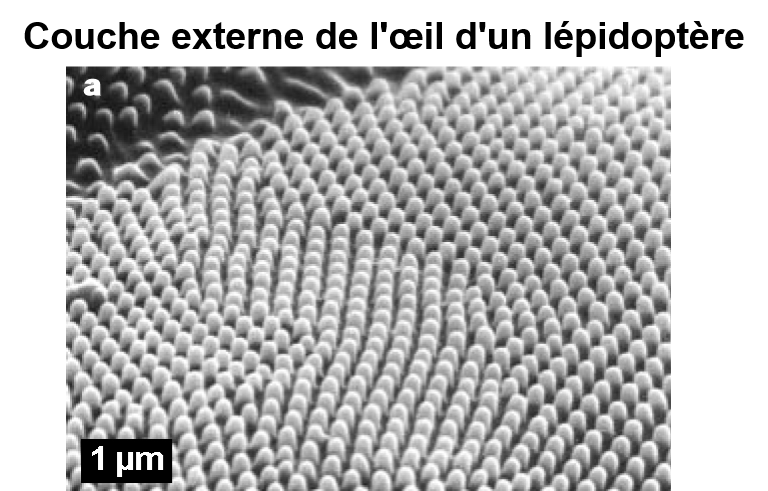
\includegraphics[scale=0.3]{M12}}. L'indice de réflexion de l'oeil d'un lépidoptère valant environ 1.5, les interstices à la surface de l'oeil diminue l'indice de réflexion à environ 1.3 puisqu'il devient plus proche de celui de l'air. Il s'agit donc du problème précédent pour lequel la couche vaut 300 nm. En outre, le gradient de cet indice de réflexion permet spécialement de minimiser la réflexion. Cette couche permet de maximiser la lumière visible rentrant dans l'oeil de l'insecte. Elle présente aussi un réel avantage pour la survie puisqu'elle n'attire pas les prédateurs qui percevraient de la lumière réfléchie. Les couches anti-reflets sur les lunettes\footnote{ou les cellules solaires, \dots} utilisent ce même principe un peu plus simplifié.
\newpage

\subsection{Couche réflectrice}

Dans le cas contraire, les ailes de certains papillons\footnote{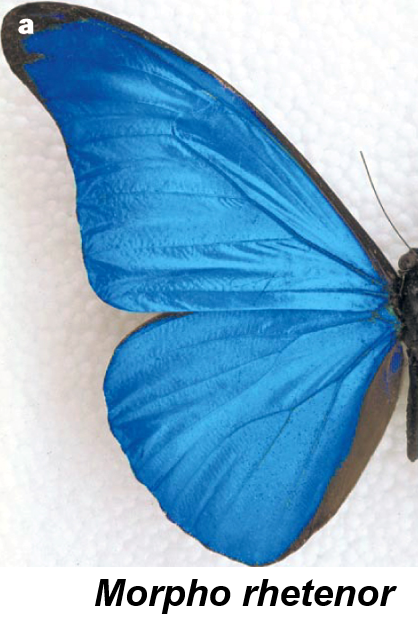
\includegraphics[scale=0.3]{M13}} peuvent être élaborées pour diffuser un maximum de lumière pour certaines couleurs. Les interférences constructives sont maximisées dans le bleu pour que le \textit{Morpho rhetenor} soit vu à 700 m (avantage reproductif).	Par ailleurs, les réflexions désorientent les prédateurs (avantage pour la survie). Les couches réfléchissant la chaleur\footnote{liée à la transmission des rayons infra-rouges} tirent profit ce principe.

\subsection{L'interféromètre de Michelson-Morley}

Michelson était un scientifique de la fin du 19e siècle qui s'est beaucoup intéressé au calcul de la vitesse de la lumière. A cette époque, les gens pensaient que celle-ci se déplaçaient dans un certain milieu\footnote{Personne n'avait encore réussi à le détecter} appelé l'éther. Michelson a donc essayé de calculer la vitesse de la lumière dans cet éther pour prouver son existence. Son raisonnement est établi par analogie avec la vitesse du son qui diffère suivant la direction du vent. Le temps pour faire un aller-retour est légèrement plus court pour la direction perpendiculaire au vent que la direction parallèle. 

\begin{figure}[htb]
\centering
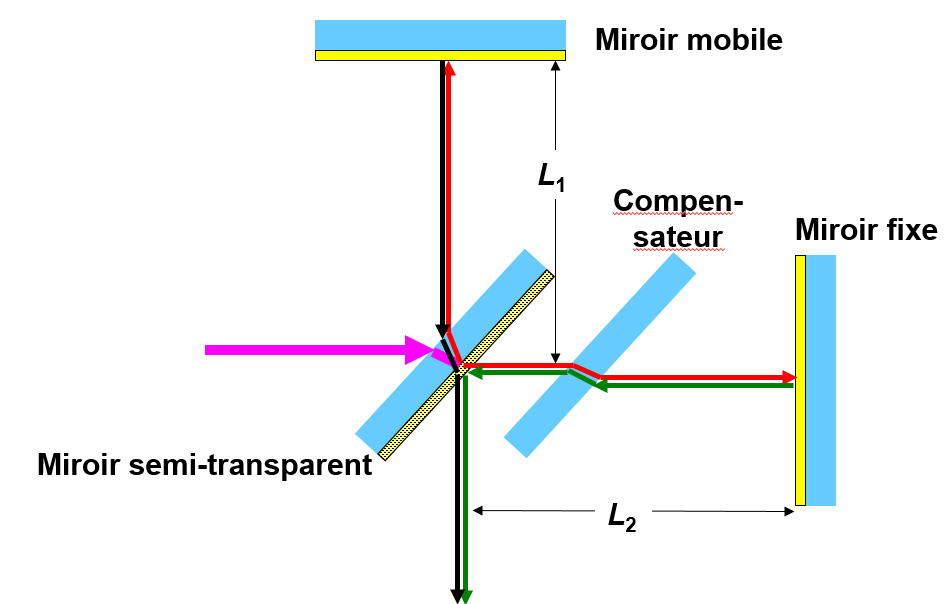
\includegraphics[scale=0.3]{M14}
\caption{Interféromètre de Michelson}
\label{fig:Michelson}
\end{figure}

Puisque la Terre tourne autour d'un axe fixe, la lumière devrait avoir deux vitesses différentes suivant que son trajet se déroule parallèlement ou perpendiculairement à l'axe rotation de la Terre.  Il a donc mesuré les temps mis par chaque trajet en analysant les signaux d'interférences additionnés et projetés sur le miroir fixe.

Michelson n'a jamais pu mettre en évidence une différence entre les deux trajets. Ce résultat négatif a amené Lorentz et Einstein à postuler l'inexistence de l'éther et l'invariance de la vitesse de la lumière.


\section{Intensité de la figure d'interférence}

Dans certains cas, il faut non seulement identifier les conditions d'interférence constructive ou destructive, mais aussi calculer l'intensité de l'onde résultante à différents points de l'espace. Ceci est plus difficile que ce que nous avons fait jusqu'ici, puisqu'il faut additionner les champs, puis calculer l'intensité de l'onde résultante\footnote{pour rappel, l'intensité d'une onde est le flux moyen d'énergie passant par unité de surface dans la direction de propagation de l'onde}.
 % On peut aussi le calculer en évaluant la norme du vecteur de Poynting $E\times H$ moyenné sur une durée beaucoup plus grande que la période.

Pour simplifier le calcul, il est utile de passer à une représentation différente des ondes sinusoïdales, une représentation sous forme complexe. Considérons une onde électromagnétique de la forme\footnote{il est toujours possible de l'écrire localement sous cette forme, en choisissant correctement son repère; si l'onde est sphérique, $A$ est une fonction de la distance à la source, $x$, mesurée le long d'un rayon; si l'onde est plane, $A$ est une constante} $\overset\rightarrow{\mbox{E}}(x,y,z)=A\cos(kx-\omega t)\overset\rightarrow{\mbox{l}_z}$. Il est évident que nous pouvons aussi écrire:
$$\overset\rightarrow{E}(x,y,z)=\operatorname{Re}\Big((A\exp\big(j(kx-\omega t)\big)\overset\rightarrow{\mbox{l}_z}\Big)=\operatorname{Re}\Big(\overset\rightarrow{E_c}(x,y,z)\Big)$$
où $\operatorname{Re}(c)$ désigne la partie réelle d'un nombre complexe et $j$ est la racine carrée de $-1$. Écrire l'onde $\overset\rightarrow{E}$ sous cette forme revient en fait à la considérer comme la projection sur l'axe réel d'un champ complexe $\overset\rightarrow{E}_c$ tournant dans un plan imaginaire\footnote{\includegraphics[scale=0.4]{10}} sans existence physique. Le plan bleu n'existe pas dans notre réalité puisqu'il est purement imaginaire.

Comme la fonction $\operatorname{Re}()$ est linéaire, nous pouvons travailler dans un problème d'interférence avec les champs complexes tournants, les additionner, et prendre la partie réelle du total à la fin du calcul. Dans ce cas, nous oublions en général que le champ électrique est réel, nous le remplaçons par son expression complexe, et ce n'est qu'en bout de course que nous en gardons la partie réelle.

Cette approche est utilisée pour plusieurs raisons. Tout d'abord, il est souvent plus facile d'additionner des exponentielles complexes que des cosinus. En effet, il est en général plus simple de mettre des facteurs communs en évidence avec des exponentielles. Par ailleurs, le calcul de l'intensité du champ est également aisé dans ce domaine, puisqu'il nous suffit maintenant de prendre le produit scalaire du champ complexe et de son complexe conjugué\footnote{à un facteur multiplicatif près, dépendant de l'impédance caractéristique de l'onde, voir chap. 3}.
% !! check reference
En effet, l'intensité de l'onde est proportionnelle au carré de l'amplitude du champ électrique, $A^2$.
\begin{align*}
I & = \frac{\epsilon c}{2}\overset\rightarrow{E_c}.\overset\rightarrow{E_c^*} \\
& = \frac{\epsilon c}{2}\Big((A\exp\big(j(kx-\omega t)\big)\overset\rightarrow{\mbox{l}_z}\Big).\Big((A\exp\big(-j(kx-\omega t)\big)\overset\rightarrow{\mbox{l}_z}\Big) \\
& = \frac{\epsilon c}{2}A^2
\end{align*}

De plus,  cette notation complexe facilite le calcul des phénomènes ondulatoires dans des milieux absorbants ou conducteurs. 

Et finalement, le champ complexe est l'analogue de la fonction d'onde utilisée en physique quantique\footnote{dans la seconde partie de ce cours LFSAB1203}.

Graphiquement, la figure \ref{M1} illustre la somme de deux ondes représentées par leurs vecteurs tournants, $\overset\rightarrow{E}=\overset\rightarrow{E_1}+\overset\rightarrow{E_2}$, dont l'une est en avance par rapport à l'autre \footnote{l'angle formé entre les deux vecteurs tournants est le déphasage angulaire}:
\begin{figure}[htb]
\centering
\includegraphics[scale=0.8]{M1}
\caption{Addition de 2 champs vectoriels complexes}
\label{M1}
\end{figure}

Utilisons à présent ce formalisme pour résoudre quantitativement un problème d'interférence. Un écran percé de $N$ fentes infiniment étroites séparées les unes des autres par la distance $d$, est illuminé par une onde plane\footnote{dans le plan $(x,y)$} arrivant sous incidence normale (voir fig. \ref{M2}).
\begin{figure}[htb]
\centering
\includegraphics[scale=0.7]{M2}
\caption{Schéma des interférences issues d'une onde plane au travers d'un réseau de $N$ fentes}
\label{M2}
\end{figure}

\begin{marginfigure}[0cm]
	\includegraphics[scale=1]{M3}
	\caption{Retard de phase}
	\label{fm3}
\end{marginfigure}

Par l'approximation de Fraunhofer, le point $P$ où nous voulons calculer l'intensité se trouve très loin de l'écran. Nous pouvons alors considérer que les faisceaux bleus sont pratiquement parallèles. Chaque faisceau accuse un retard $d'$ par rapport au faisceau supérieur voisin (fig \ref{fm3}). La distance entre la source $S_p$ ($p=1,\ldots, N$) et le point $P$ est $R+(p-1)d'$.

Au point $P$, la superposition des faisceaux donne :
\begin{align*}
\overset\rightarrow{E}(P) & = \sum\limits_{p=1}^N \frac{A}{R+(p-1)d'}\exp\bigg(j\Big(k\big(R+(p-1)d'\big)-\omega t\Big)\bigg)\:\overset\rightarrow{\mbox{l}_z} \\
& = \exp\Big(j(kR-\omega t)\Big)\:\overset\rightarrow{\mbox{l}_z}\: \sum\limits_{p=1}^N \frac{A}{R+(p-1)d'}\exp(jk(p-1)d')
\end{align*}

Cette expression est simplement la somme des $N$ ondes sphériques émises par chaque fente, avec un repère placé de telle sorte que les champs soient parallèles à $\overset\rightarrow{\mbox{l}_z}$ en $P$. Le symbole $k$ est le nombre d'onde, $2\pi$ divisé par la longueur d'onde. Évidemment, le champ électrique correspond seulement à la partie réelle de cette expression, mais par souci de simplicité nous admettons que le symbole $\operatorname{Re}()$ est implicite dans ce qui suit.

Maintenant, la seule chose qu'il reste à faire est un développement mathématique de cette expression. Tout d'abord, l'approximation de Fraunhofer implique que $d' \ll R$. Dans ce cas, on peut considérer que 
$$\frac{A}{R+(p-1)d'} \simeq \frac{A}{R}.$$ 
Cette approximation n'est pas valide dans l'argument des exponentielles $jk(p-1)d' $, puisqu'une différence d'une demi-longueur d'onde est évidemment très importante quand il s'agit d'additionner des cosinus \footnote{ou des exponentielles complexes}. 
En se rappelant de la relation
$$\sum\limits_{p=0}^{N-1} x^p=\frac{1-x^N}{1-x}, $$
on écrit alors:
\begin{align*}
\overset\rightarrow{E}(P) & = \frac{A\exp\Big(j(kR-\omega t)\Big)}{R}\:\overset\rightarrow{\mbox{l}_z}\: \sum\limits_{p=1}^N \exp\Big(jk(p-1)d'\Big) \\
& =\frac{A\exp\Big(j(kR-\omega t)\Big)}{R}\:\overset\rightarrow{\mbox{l}_z}\: \sum\limits_{p=0}^{N-1} \exp(jkpd') \\
& = \frac{A\exp\Big(j(kR-\omega t)\Big)}{R}\:\overset\rightarrow{\mbox{l}_z}\: \sum\limits_{p=0}^{N-1} {\Big(\exp(jkd')\Big)}^{p} \\
& = \frac{A\exp\Big(j(kR-\omega t)\Big)}{R}\:\overset\rightarrow{\mbox{l}_z}\: 
\frac{1-{\Big(\exp(jkd')\Big)}^N}{1-\exp(jkd')}\\
& = \frac{A\exp\Big(j(kR-\omega t)\Big)}{R}\:\overset\rightarrow{\mbox{l}_z}\: 
\frac{1-\exp(jkNd')}{1-\exp(jkd')}
\end{align*}

Puisque $\exp(j\theta)+\exp(-j\theta)= 2\cos(\theta),$ l'intensité de l'onde résultante en $P$ est donnée par:
\begin{align*}
I(P) & =\frac{\epsilon c}{2}\overset\rightarrow{E_c}.\overset\rightarrow{E_c^*} \\
& = \frac{\epsilon c}{2}\frac{A^2}{R^2}\frac{\Big(1-\exp(jkNd')\Big)\Big(1-\exp(-jkNd')\Big)}{\Big(1-\exp(jkd')\Big)\Big(1-\exp(-jkd')\Big)}\\
& = \frac{\epsilon c}{2}\frac{A^2}{R^2}\frac{1-\exp(jkNd')-\exp(-jkNd')+1}{1-\exp(jkd')-\exp(-jkd')+1}\\
& = \frac{\epsilon c}{2}\frac{A^2}{R^2}\frac{2-2\cos(kNd')}{2-2\cos(kd')}\\
& = \frac{\epsilon c}{2}\frac{A^2}{R^2}\frac{1-\cos(kNd')}{1-\cos(kd')}\\
& = \frac{\epsilon c}{2}\frac{A^2}{R^2}\frac{2\sin^2(\frac{kNd'}{2})}{2\sin^2(\frac{kd'}{2})}\\
& = \frac{\epsilon c}{2}\frac{A^2}{R^2}\frac{\sin^2(\frac{N\pi d\sin\theta}{\lambda})}{\sin^2(\frac{\pi d\sin\theta}{\lambda})}
\end{align*}

Cette expression montre que l'intensité diminue en fonction du carré de la distance entre les fentes et le point $P$. De plus, le numérateur passe régulièrement par zéro, chaque fois que $N\pi d\sin\theta/\lambda$ vaut un multiple de $\pi$, c'est-à dire quand 
$$  d\sin\theta=\frac{m}{N}\lambda$$
où $m$ est un nombre entier. Ces conditions correspondent en général à des situations dans lesquelles les ondes interfèrent globalement de manière destructive, sauf pour une série de cas particuliers. Ces cas particuliers correspondent aux conditions $$d\sin \theta=n\lambda$$
où $n$ est un autre nombre entier. Si cette condition supplémentaire est vérifiée, le dénominateur de l'expression précédente tend vers zéro également, et la limite du quotient vaut\footnote{pour $\theta$ tendant vers $0$, le résultat étant similaire pour les autres pics}
\begin{align*}
\lim\limits_{\theta \rightarrow 0}\frac{\sin^2(\frac{N\pi d\sin\theta}{\lambda})}{\sin^2(\frac{\pi d\sin\theta}{\lambda})} & \overset{\frac{0}{0}}{=}\lim\limits_{\theta \rightarrow 0}\frac{2\sin(\frac{N\pi d\sin\theta}{\lambda})\frac{N\pi d\cos\theta}{\lambda}}{2\sin(\frac{\pi d\sin\theta}{\lambda})\frac{\pi d\cos\theta}{\lambda}} \\
& =\lim\limits_{\theta \rightarrow 0}\frac{\sin(\frac{N\pi d\sin\theta}{\lambda})N}{\sin(\frac{\pi d\sin\theta}{\lambda})}\\
& \overset{\frac{0}{0}}{=}\lim\limits_{\theta \rightarrow 0}\frac{\cos(\frac{N\pi d\sin\theta}{\lambda})\frac{N^2\pi d\cos\theta}{\lambda}}{\cos(\frac{\pi d\sin\theta}{\lambda})\frac{\pi d\cos\theta}{\lambda}}\\
& = N^2.
\end{align*}

L'intensité est alors $(\epsilon c/2)(NA/R)^2$, et les ondes interfèrent toutes ensemble de manière constructive en $P$. Ces directions correspondent à des maxima et la largeur du lobe\sidenote[][-1cm]{\includegraphics[scale=0.3]{M15}} associé est déterminé par
$$d\sin\theta/\lambda=2/N,$$
un nombre élevé de fentes ($N\uparrow\uparrow$) engendre donc des raies très étroites ($\theta\downarrow\downarrow$). Un nombre élevé des fentes implique aussi des maximas très élevés. Il est utile de se souvenir que, puisque ces maximas correspondent toujours à une situation où les $N$ sources sont en phase, ce maximum correspond toujours à une amplitude $N$ fois plus grande, et donc une intensité $N^2$ fois plus grande que ce qui serait reçu avec une seule source.

La figure \ref{M4} représente graphiquement l'intensité pour $10$ fentes.
\begin{figure}[htb]
\centering
\includegraphics[scale=0.33]{M4}
\caption{Graphique de l'intensité selon l'angle de direction par rapport à la normale d'une onde passant à travers un réseau de 10 fentes }
\label{M4}
\end{figure}

Il y a un grand nombre de possibilités de combiner les différents faisceaux pour arriver à une intensité nulle, tandis que les cas correspondant à l'interférence constructive de tous les faisceaux sont plus rares. Nous avons considéré des fentes infiniment étroites; en général, il faut prendre en compte une largeur finie de fente, et un facteur supplémentaire s'introduit dans les expressions \footnote{voir chapitre lié à la diffraction}.


	%\documentclass[a4paper,justified]{tufte-book}
\chapter{Diffraction} %% created by Martin Braquet

La largeur des fentes n'est pas prise en compte dans le chapitre précédent et conduit à une approximation du phénomène physique. Une fente de largeur finie ne peut pas se représenter comme une unique source d'ondes. La \textit{diffraction} est le comportement non idéal des ondes lorsqu’elles rencontrent un obstacle ou une ouverture.

\begin{figure}[h]
    \centering
    \includegraphics[scale=0.4]{M20}
    \caption{Projet de construction de deux télescopes européens}
    \label{tele}
\end{figure}

\noindent Les 4 télescopes optiques (voir fig \ref{tele})
nommés \textit{VLT} (européens) implantés au Chili ont chacun un diamètre de 8,2 m.
L'amélioration de la précision des télescopes nécessite d'augmenter leur diamètre. La diffraction explique ce constat le long de ce chapitre.

\section{Diffraction par une fente de petite taille}

On considère un rayon lumineux dirigé vers une plaque opaque percée d'une fente de forme rectangulaire d'une largeur de l'ordre du micromètre. Le rayon est dévié dans toutes les directions qui sont dans le demi-cercle opposé à l'apparition du rayon. On remarque sur la figure \ref{d1} que l'intensité dépend de l'angle $\theta$ de la déviation du rayon par rapport à la direction initiale du rayon incident. Contrairement au chapitre précédent, l'intensité est nulle lorsque $\theta$ tend vers $\pm \pi/2$, ce constat est en accord avec les expériences réalisées au cours.

\begin{figure}[h]
    \centering
    \includegraphics[scale=0.5]{M21}
    \caption{Diffraction par une fente de petite taille}
    \label{d1}
\end{figure}


\noindent Par le principe de Huygens, l'onde traversant cette petite fente peut être remplacée par un ensemble de toutes petites sources les unes à côté des autres et rayonnant dans toutes les directions. Supposons que l'on a $N$ petites sources séparées d'une distance $d$ couvrant la largeur $a=Nd$ de la fente.

\begin{figure}[h]
    \centering
    \includegraphics[scale=0.6]{M23}
    \caption{Diffraction par une fente de petite taille, représentée par $N$ sources}
    \label{f2}
\end{figure}

\noindent Sur la figure \ref{f2}, on calcule l'intensité en $P$ résultant de la somme des ondelettes. Le problème est formellement identique à celui traité pour le cas de N fentes idéales.

\noindent Néanmoins, en réalité le nombre de sources $N$ n'est pas fini. On adapte donc la formule de l'intensité pour un réseau de fentes du chapitre sur les interférences en faisant tendre vers $0$ la distance $d$ entre les sources tout en gardant la largeur de le fente $a=dN$ constante. Puisque le nombre de sources est augmenté, il convient de diminuer l'amplitude de chacune de ces sources de manière à conserver la somme des amplitudes: $A \rightarrow A/N=Ad/a$.

\begin{align*}
I(P) & =I_0\lim_{d\to 0} \frac{d^2}{a^2}\frac{\sin^2(\frac{Nd\pi \sin\theta}{\lambda})}{\sin^2(\frac{\pi d\sin\theta}{\lambda})}\\
& \overset{\frac{0}{0}}{=} I_0\lim_{d\to 0} \frac{\sin^2(\frac{a\pi \sin\theta}{\lambda})}{a^2}\frac{2d}{2\sin(\frac{d\pi \sin\theta}{\lambda})\cos(\frac{d\pi \sin\theta}{\lambda})\frac{\pi \sin\theta}{\lambda}}\\
& =I_0 \lim_{d\to 0} \frac{\sin^2(\frac{a\pi \sin\theta}{\lambda})}{a^2}\frac{2d}{\sin(2\frac{d\pi \sin\theta}{\lambda})\frac{\pi \sin\theta}{\lambda}}\\
& \overset{\frac{0}{0}}{=}I_0 \lim_{d\to 0} \frac{\sin^2(\frac{a\pi \sin\theta}{\lambda})}{a^2}\frac{2}{\cos(2\frac{d\pi \sin\theta}{\lambda})2(\frac{\pi \sin\theta}{\lambda})^2}\\
& =I_0 \frac{\sin^2(\frac{\pi a \sin\theta}{\lambda})}{(\frac{\pi a \sin\theta}{\lambda})^2}.
\end{align*}

\begin{figure}[h]
\includegraphics[scale=0.6]{M25}
\caption{Intensité d'un rayon lumineux traversant une fente}
\label{f3}
\end{figure}

\noindent Cette équation montre qu'une grande fente génère des lobes plus étroits. L'intensité, présentée sur la figure \ref{f3}, s'annule lorsque
$$
  \frac{\pi a \sin\theta}{\lambda}=m\pi \Rightarrow a \sin\theta = m\lambda \qquad(\forall m\in  \mathbb{Z}_0).
$$

\noindent Cette relation permet donc de mesurer la largeur d'une fente (ou on le verra plus tard, d'un objet). En mesurant expérimentalement l'angle donnant lieu au premier lobe, $a$ peut être déterminé.

\noindent On pourrait également vouloir calculer les positions des maxima locaux d'intensité. Contrairement à ce qu'une observation rapide de l'équation ci-dessus pourrait laisser penser, les pics ne se produisent pas exactement quand la fonction sinus vaut $\pm1$. La dérivée de l'intensité par rapport à $\theta$ est une équation transcendante qui s'annule à des positions correspondant à un maximum pour 
\[
\frac{2\pi}{\lambda}a \sin\theta\simeq
\left\{
\begin{array}{c}
 2,86\pi\\
 4,92\pi\\
...
\end{array}
\right.
\Longrightarrow
I\simeq
\left\{
\begin{array}{c}
 0,0472I_0 \mbox{ (1er pic)}\\
 0,0165I_0 \mbox{ (2e pic)}\\   
  ...
\end{array}
\right.
\]
Ces intensité diminuent très rapidement, le premier pic valant seulement $5\%$ du pic central. Dans les chapitres suivants, on approximera donc parfois la figure de diffraction par un unique lobe.

\section{Diffraction par un objet de petite taille}

Il est possible de montrer que la lumière est diffractée de la même façon en traversant une fente ou un objet de même taille. Pour prouver cela, on considère d'abord, selon le principe de Huygens, et pour une onde se propageant dans le vide (sans obstacle), la représentation d'un front d'onde par une multitude de petites sources (fig \ref{f4}). Le champ généré plus loin dans la direction de propagation de l'onde (ici vers la droite) est obtenu par la somme des ondelettes créées par chacune des petites source (les cercles turquoises sur la figure). On le dénote par $\overset\rightarrow{E}_0$.

\begin{marginfigure}[0cm]
\includegraphics[width=1\textwidth]{M26}
\caption{Représentation d'un front d'onde par une multitude de sources}
\label{f4}
\end{marginfigure}

\noindent Pour analyser les effets de diffraction d'une fente et d'un objet, on décompose ensuite ce front d'onde en deux parties (fig \ref{d2}):
\begin{itemize}
    \item l'ensemble des sources bleues se trouvant en dehors d'un petit objet de largeur $a$ et dont la somme des ondelettes transmises correspond à l'effet de diffraction par cet objet. On dénote l'onde correspondante par $\overset\rightarrow{E}_2$
    \item l'ensemble des sources rouges se trouvant à l'intérieur de la fente de largeur $a$ et dont la somme des ondelettes transmises correspond à la diffraction par cette fente. On dénote l'onde correspondante par $\overset\rightarrow{E}_1$
\end{itemize}

\begin{figure}[h]
    \centering
    \includegraphics[scale=0.4]{M27}
    \caption{Diffraction par une fente ou un objet}
    \label{d2}
\end{figure}

\noindent Par superposition, il est clair que $\overset\rightarrow{E}_1+\overset\rightarrow{E}_2=\overset\rightarrow{E}_0$. La somme correspond au champ obtenu sans obstacle. Le champ transmis $\overset\rightarrow{E}_2$ correspond au champ créé par la diffraction à travers un objet de largeur $a$ et le champ transmis $\overset\rightarrow{E}_1$ correspond au champ créé par la diffraction à travers une fente de largeur $a$ (établi au paragraphe précédent).
Si on se place en un point $P$ pour lequel $\overset\rightarrow{E}_0(P)=\overset\rightarrow{0}$, on trouve $\overset\rightarrow{E}_1(P)=-\overset\rightarrow{E}_2(P)$, et l'intensité transmise par la fente $I_1\propto |\overset\rightarrow{E}_1|^2$ est égale à l'intensité transmise par l'objet $I_2\propto |\overset\rightarrow{E}_2|^2$. Le principe de Babinet énonce de manière analogue que deux figures de diffraction identiques sont créées lors d'une diffraction par un objet ou une fente de même taille. Ainsi, tout problème de diffraction impliquant une ouverture peut être remplacé par un problème équivalent impliquant un petit objet. Puisqu'il n'y a pas de diffraction si le rayon rencontre une plaque opaque ou s'il n'y a pas d'objet, ce sont les bords qui produisent le phénomène de diffraction.

\noindent A titre d'exemple, dans le cas de la diffraction par un cheveu, on observe toujours bien l'impact du laser sur l'écran (correspondant au $\overset\rightarrow{E}_0$), auquel vient se soustraire la figure de diffraction correspondant à une fente. Il s'agit d'une soustraction en terme de champ électromagnétique. Dans toutes les zones en dehors du point d'impact du laser, on observe exactement la même intensité que pour la diffraction par une fente.


\begin{marginfigure}[2cm]
\includegraphics[width=0.9\textwidth]{M55}
\caption{Diffraction par une fente}
\label{f5}
\end{marginfigure}

\noindent Il est possible d'obtenir les directions des franges noires par un raisonnement basé sur l'interférence destructive des ondes créées par une fente de largeur $a$. La différence de chemin (fig \ref{f5}) entre l'onde émise au centre de la fente et celle émise juste en dessous du bord supérieur vaut $a/2\:\sin\theta$. Pour qu'il y ait une interférence destructive, cette distance doit valoir $(2m+1)\lambda/2$. De manière similaire, les deux faisceaux venant de deux sources, décalées d'une distance infinitésimale par rapport aux deux sources précédentes, ont la même différence de chemin et se détruisent aussi. Donc, la lumière de chaque source sur la moitié supérieure de la fente s'annule avec la source correspondante dans la moitié inférieure, donnant ainsi une frange sombre dans cette direction $\theta$. Donc $\sin\theta=\pm\lambda/a$, le signe $\pm$ indique que la figure de diffraction est symétrique. La frange en $\theta>0$ apparaît en $P$ quand la lumière de la moitié inférieure de la fente fait une distance plus grande de $\lambda/2$ que celle de la moitié supérieure. La frange en $\theta<0$ apparaît en $P$ quand la lumière de la moitié supérieure de la fente fait une distance plus grande de $\lambda/2$ que celle de la moitié inférieure. En divisant la fente non plus en 2 mais en 4,6,8, et ainsi de suite, on utilise l'argument ci-dessus pour montrer qu'une interférence destructive se produit quand $\sin\theta=\pm\lambda/a,\pm2\lambda/a,\pm3\lambda/a,\pm4\lambda/a$,...
Finalement, on peut reformuler la relation pour obtenir
$$
    \sin\theta=\frac{m\lambda}{a}\qquad(\forall m\in  \mathbb{Z}_0).
$$
qui était déjà établie auparavant.

\section{Pouvoir séparateur d'un instrument d'optique (ou pouvoir de résolution spatiale) }

La diffraction est un des effets principaux limitant la précision des instruments d'observation optiques (ou plus généralement observant des ondes).

\noindent Le microscope optique possède une lentille d'environ 5 mm de diamètre pour observer des objets visibles (correspondant à des longueurs d'onde entre 380 et 780 nm).

\noindent Le radiotélescope d'Arecibo sur la figure \ref{f6} a une parabole d'environ 305 m de diamètre focalisant les ondes électromagnétiques pour observer des objets émettant avec une longueur d'onde de 10 cm. Ce télescope situé à Porto Rico est opéré par l'Université de Cornell.

\begin{marginfigure}[-2cm]
\includegraphics[width=0.9\textwidth]{M29}
\caption{Radiotélescope d'Arecibo}
\label{f6}
\end{marginfigure}

\noindent Le rapport $\lambda/a$ entre la longueur d'onde et la taille de l'ouverture est de l'ordre de $10^{-3}$ dans les deux cas et sa raison est explicitée ci-dessous.

\noindent Dans les instruments d'optique, on considère que la lumière entre dans une lentille de diamètre $a$. Le passage dans cette ouverture circulaire génère un effet de diffraction. Son analyse mathématique s'effectue de manière presque similaire à celle d'une fente de largeur $a$. La diffraction par une ouverture circulaire engendre une figure de diffraction (appelée tache d'Airy\footnote{du physicien anglais \textit{George Biddell Airy} (1801-1892)}) formée de cercles concentriques dont l'intensité diminue avec le diamètre du cercle. 

\noindent Lorsque la figure est observée loin du trou diffractant (approximation de Fraunhofer), l'intensité varie en fonction de l'angle $\theta$ entre le point considéré et le centre de la figure comme:
$$
    I(\theta)=I_0\bigg(\frac{2J_1(\frac{\pi a\sin\theta}{\lambda})}{\frac{\pi a\sin\theta}{\lambda}}\bigg)^2
$$
où $J_1$ est la fonction de Bessel du premier ordre, $I_0$ est l'intensité au centre de la figure et $\theta$ est l'angle entre l'axe de révolution et la direction considérée.

\noindent La première annulation de cette fonction se produit lorsque 
$$
    a\sin\theta\simeq1,22\lambda.
$$
Cette relation montre que si le rapport $\lambda/a$ est identique pour deux expériences, la même figure de diffraction sera représentée. Les deux cercles sombres suivants sont situés dans les directions $\theta$ vérifiant les relations $a\sin\theta\simeq2,23\lambda$ et $a\sin\theta\simeq3,24\lambda$.

\noindent L'intensité diminue plus rapidement que dans une fente rectangulaire, le pic d'intensité du premier ordre valant seulement $1,7\%$ de l'intensité au centre de la figure. La plupart ($85\%$) de l'énergie lumineuse est située dans le disque central (disque d'Airy).

\noindent Pour analyser le pouvoir de séparation d'un instrument d'observation, on considère deux rayons lumineux traversant un trou dans une boite, leur rayon incident n'est pas perpendiculaire à la face possédant le trou (voir fig \ref{d4}).

\begin{figure}[h]
    \centering
    \includegraphics[scale=0.5]{M30}
    \caption{Rayons lumineux traversant un creux dans une boite}
    \label{d4}
\end{figure}

\noindent La figure \ref{d6} illustre la projection des taches de lumière sur la face opposée au creux pour un diamètre $a$ décroissant vers les images de droite.

\begin{figure}[h]
    \centering
    \includegraphics[scale=0.4]{M31}
    \caption{Taches de lumières pour différents diamètres}
    \label{d6}
\end{figure}

\noindent Puisque la largeur des lobes est inversement proportionnelle au diamètre $a$, les taches s'agrandissent avec la diminution du diamètre du creux. Par contre, les taches gardent le même centre car l'angle d'incidence ne change pas.
Les taches deviennent ainsi indissociables en dessous d'une certaine valeur de $a$. 

\noindent De la même manière, on peut également varier la distance $d$, c'est-à-dire l'angle d'incidence des deux rayons. La figure \ref{d8} présente les taches avec la distance $d$ qui diminue vers les images de droite.

\begin{figure}[h]
    \centering
    \includegraphics[scale=0.47]{M32}
    \caption{Taches de lumières pour différents angles d'incidence}
    \label{d8}
\end{figure}

\noindent Contrairement à l'expérience précédente, le diamètre des taches, lié à $a$, ne varie pas mais les positions des centres se rapprochent lorsque $d$ diminue. Pour une taille de trou donnée, il y a une distance $d$ (et un angle d'incidence $\theta$) minimum pour laquelle les taches ne se superposent pas. 

\noindent Pour un œil, il y a aussi l’effet de la lentille qui fait converger les faisceaux vers le même point, excepté les diffractés. Sans cette convergence, il y aurait superposition de la tache qui passe, et des effets de diffraction. Mais la focalisation résultant de la lentille permet de réduire la tache éclairée, et il ne reste plus que l’effet de diffraction.

\begin{marginfigure}[0cm]
\includegraphics[width=0.9\textwidth]{M33}
\caption{Critère de Rayleigh}
\label{f7}
\end{marginfigure}

\noindent Une relation mathématique peut s'établir en déterminant un critère de résolution (fig \ref{f7}) énoncé par Lord Rayleigh: deux taches sont résolues si le premier lobe de la figure de diffraction d'un des deux faisceaux ne se chevauche pas avec le centre de l'autre rayon lumineux. Cela correspond à la résolution angulaire minimale sous laquelle les deux objets formeront une seule tache. Pour augmenter la résolution en gardant la même distance entre le trou et l'objet ($d$ constant), il faut ainsi augmenter $a$ et/ou diminuer $\lambda$.

\noindent Ainsi, pour discerner les disques lumineux, l'angle d'incidence $\theta_i$ doit être supérieur à l'angle du premier lobe de diffraction $\theta_1$:
$$
    \sin\theta_i>\sin\theta_1
$$
$$
    \sin\theta_i>1,22\lambda/a.
$$
En posant $L$, la distance entre le trou et les deux sources, on peut approximer cette relation pour des petits angles d'incidence tels que $\sin\theta_i=\tan \theta_i$:
$$
    \tan\theta_i=d/L>1,22\lambda/a.
$$

\subsection{Microscopie optique de haute résolution}

\begin{marginfigure}[-1.5cm]
\includegraphics[width=0.9\textwidth]{M34}
\caption{Microscope optique}
\label{f8}
\end{marginfigure}

Les caractéristiques d'un microscope optique (fig \ref{f8}) sont les suivantes: $\lambda\simeq500nm,a\simeq2mm$ et $L\simeq1mm$. La distance de résolution vaut ainsi 
$$
d_{min}=1,22\lambda L/a\simeq300\:nm.
$$
Pour que ce microscope puisse discerner les atomes ($d\simeq0,5nm$), la longueur d'onde devrait être inférieure à $da/(1,22L)\simeq1nm$ (rayons X). Puisqu'il n'existe pas de lentille qui puisse analyser les rayons X, un tel microscope n'est pas assez précis pour voir des atomes.

\subsection{Microscopie électronique de haute résolution}

\begin{marginfigure}[-1cm]
\includegraphics[width=0.9\textwidth]{M35}
\caption{Microscope électronique}
\label{f9}
\end{marginfigure}

Pour améliorer la précision, on peut remplacer les ondes lumineuses par des électrons (fig \ref{f9}), qui ont aussi des propriétés ondulatoires. La longueur d'onde d'un électron est beaucoup plus petite (entre\footnote{cette longueur d'onde dépend de la tension d'accélération des électrons} $0,1$ et $1nm$). Ce dispositif, qui n'exploite plus les ondes visibles, analyse un objet de manière indirecte. Le microscope enregistre ainsi des données électroniques pour les convertir ensuite en une représentation 2D ou 3D. Un microscope électronique à transmission a une résolution de $$d_{min}=1,22\lambda L/a\simeq0,5\:nm$$ puisque $a\simeq L\simeq10mm$.
Néanmoins, il est nettement plus cher et requiert des lentilles magnétiques pour focaliser le faisceau d'électrons.

\begin{marginfigure}[0cm]
\includegraphics[width=0.9\textwidth]{M36}
\caption{Image d'un échantillon de graphène}
\label{f10}
\end{marginfigure}

\noindent Ce microscope produit par exemple une image précise d'un échantillon de graphène (fig \ref{f10}), un matériau dont la distance interatomique vaut environ $0,15$ nm.

\noindent D'autres principes d'imagerie existent également: microscopes à force atomique, microscopes à effet tunnel,...

\subsection{Microlithographie et nanolithographie}

\begin{marginfigure}[0cm]
\includegraphics[width=0.9\textwidth]{M37}
\caption{Photolitographie}
\label{f11}
\end{marginfigure}

La microlithographie et la nanolithographie sont deux procédés de fabrication très précise d'objets. Ce système est principalement utilisé pour créer des circuits intégrés dans le domaine de l'électronique. Le substrat est composé d'une couche de polymère photo-sensible (résine) sur un disque en silicium. Pour tracer le circuit, on illumine ce substrat au travers d'un masque réalisé au préalable, ce qui a pour effet de modifier la résine à des endroits précis sur la couche de polymère. Le substrat est ensuite rincé par un solvant sélectif pour enlever les parties du polymère qui ont été exposées aux rayons. On peut ensuite procéder à l'implantation d'ions dans le semiconducteur aux endroits désirés afin de créer le circuit électronique voulu. 

\noindent Le masque en chrome, permettant d'exposer uniquement certaines parties du polymères, agit comme un réseau de fentes et provoque donc la diffraction des ondes. La diffraction limite la précision du circuit car les zones irradiées sur le polymère sont plus grandes que les fentes sur le cache (fig \ref{d9} a). Pour augmenter la densité de transistors par unité de surface,
il faut diminuer l'effet de diffraction, c'est-à-dire l'angle du premier lobe $\theta$. Puisqu'on ne peut pas augmenter la largeur de la fente sans diminuer la précision, il convient d'employer des ondes possédant une longueur d'onde la plus petite possible. La lithographie optique utilise les ondes lumineuses alors que la lithographie électronique (uniquement en laboratoire à l'heure actuelle) utilise des électrons pour leur faible longueur d'onde. La figure \ref{d9} b présente différentes ondes utilisées en correspondance avec leur précision.

\noindent Cette problématique apparaît de façon similaire dans la lecture des CDs et DVDs. Le lecteur optique possède une ouverture (lentille) et est sujet à une certaine diffraction qui limite la précision avec laquelle on peut lire les trous sur le CD. C'est la raison pour laquelle la technologie Blu-ray a évolué vers l'utilisation de lasers de lecture violets (longueur d'onde 400 nm) au lieu de lasers rouges (longueur d'onde 650 nm); ainsi qu'une augmentation de la taille de la lentille.

\begin{figure}[h]
\centering
\subfloat[]{\includegraphics[width=4cm]{M38}}
        \quad
\subfloat[]{\includegraphics[width=5cm]{M39}}
\caption{Lithographie}
        \label{d9}
\end{figure}

\begin{marginfigure}[0cm]
\includegraphics[width=0.9\textwidth]{M40}
\caption{Dessin d'un palmier}
\label{f13}
\end{marginfigure}

\noindent Cette technique est aussi utilisé en science des matériaux pour sculpter très finement la matière. Des chercheurs (fig \ref{f13}) à l'UCL ont par exemple créé le dessin d'un palmier très précis sur une plaque de $50\:\mu m$ de coté.

\section{Réseaux de fentes}

\begin{marginfigure}[0cm]
\includegraphics[width=0.9\textwidth]{M48}
\caption{Réseau de fentes}
\label{f12}
\end{marginfigure}

Un réseau de fentes (fig \ref{f12}) est un dispositif optique composé d'une série de fentes parallèles espacées de manière régulière.

\subsection{Analyse mathématique}

Comme illustré sur les figures \ref{d10}, on considère un réseau de $N$ fentes de largeur finie $a$ et de période $d$. Pour rappel, le principe de Huygens énonce que chaque fente se comporte comme la source d'une infinité d'ondelettes. On souhaite donc calculer l'intensité de l'onde résultante en un point $P$ en additionnant les ondes arrivant en P (avec le déphasage propre à chaque ondelette).

\begin{figure}[h]
\centering
\subfloat[]{\includegraphics[width=5cm]{M41}}
        \quad
\subfloat[]{\includegraphics[width=4cm]{M42}}
\caption{Réseau de fentes}
        \label{d10}
\end{figure}

\noindent En notation complexe, le champ généré par une ondelette (source infinitésimale) en $P$ vaut
$$
 \overset\rightarrow{dE}(P)=\frac{A}{R(z)}\frac{dz}{a}\exp\big(j(kR(z)-\omega t)\big)\overset\rightarrow{\mbox{l}_y}
$$
où $\overset\rightarrow{\mbox{l}_y}$ est un vecteur unitaire perpendiculaire au plan, $A$ est l'amplitude de l'onde plane incidente, $k$ est le nombre d'onde et $R(z)$ est la distance entre la source de l'ondelette et $P$.

Au delà de la fente, l'amplitude décroit en $1/R$ puisque l'onde est sphérique. Le facteur $dz/a$ normalise l'amplitude pour que l'intensité dans le cas idéalisé sans diffraction (une source par fente) soit identique à la somme des intensités des sources dans une même fente:
$$
 \int_0^a\frac{A}{aR(z)}\exp\big(j(kR-\omega t)\big)dz\:\overset\rightarrow{\mbox{l}_y}=\frac{A}{R(z)}\exp\big(j(kR-\omega t)\big)\overset\rightarrow{\mbox{l}_y}=\overset\rightarrow{E_{ideal}}(P)
$$
si $R$ est le même pour chaque source.

\begin{marginfigure}[0cm]
\includegraphics[width=0.9\textwidth]{M43}
\caption{Différence de chemin}
\label{f14}
\end{marginfigure}

\noindent Le champ résultant en $P$ se calcule en sommant les sources dans les $N$ fentes:
$$
  \overset\rightarrow{E(P)}=\sum_{n=0}^{N-1}\int_{nd}^{nd+a}\frac{A}{aR(z)}\exp\big(j(kR(z)-\omega t)\big)dz\:\overset\rightarrow{\mbox{l}_y}.
$$
Par l'approximation de Fraunhofer, $P$ est à l'infini et tous les rayons sont parallèles. En utilisant la figure \ref{f14}, on déduit que la direction des rayons est donnée par l'angle $\theta$ et 
$R(z)=R(z=0)+z\sin \theta$. En considérant\footnote{simplification explicitée dans le chapitre sur les interférences} $\frac{1}{R(z)}\simeq\frac{1}{R(z=0)}$,
le champ s'écrit
\begin{align*}
\overset\rightarrow{E}(P) & = \sum_{n=0}^{N-1}\int_{nd}^{nd+a}\frac{A}{aR_0}\exp\big(j(k(R_0+z\sin \theta)-\omega t)\big)dz\:\overset\rightarrow{\mbox{l}_y}\\
 &= \frac{A}{aR_0}\exp\big(j(kR_0-\omega t)\big)\sum_{n=0}^{N-1}\int_{nd}^{nd+a}\exp\big(jkz\sin \theta\big)dz\:\overset\rightarrow{\mbox{l}_y}.
\end{align*}
On peut effectuer l'intégrale et obtenir
\begin{align*}
\int_{nd}^{nd+a}\exp\big(jkz\sin \theta\big)dz & =\frac{1}{jk\sin\theta}\Big[\exp\big(jkz\sin \theta\big)\Big]_{nd}^{nd+a}\\
&=\frac{1}{jk\sin\theta}\bigg(\exp\big(jk(nd+a)\sin \theta\big)-\exp\big(jknd\sin \theta\big) \bigg)\\
&=\frac{\exp\big(jka\sin \theta\big)-1 }{jk\sin\theta}\exp\big(jknd\sin \theta\big).
\end{align*}
En utilisant la relation
$$\sum\limits_{p=0}^{N-1} x^p=\frac{1-x^N}{1-x}, $$
on transforme la somme en
\begin{align*}
\sum_{n=0}^{N-1}\exp\big(jknd\sin \theta\big)&=\frac{1-\exp\big(jkNd\sin \theta\big)}{1-\exp\big(jkd\sin \theta\big)}
\end{align*}
pour obtenir la formulation finale du champ résultant $\overset\rightarrow{E}(P)$:
$$
  \overset\rightarrow{E(P)}=\frac{A}{aR_0}\exp\big(j(kR_0-\omega t)\big)\frac{\exp\big(jka\sin \theta\big)-1 }{jk\sin\theta}\:\frac{1-\exp\big(jkNd\sin \theta\big)}{1-\exp\big(jkd\sin \theta\big)}  \:\overset\rightarrow{\mbox{l}_y}.
$$
On calcule ensuite l'intensité du champ en $P$: $I(P)=\frac{\epsilon c}{2}\overset\rightarrow{E}(P).\overset\rightarrow{E^*}(P)$. $\overset\rightarrow{E}(P)$ est un produit de 4 termes dont on peut analyser séparément l'intensité:
\begin{enumerate}
    \item $(A/aR_0)^2$
    
    \item $\exp\big(j(kR_0-\omega t)\big)\exp\big(-j(kR_0-\omega t)\big)=1$
    
    \item 
    \begin{align*}
\frac{\exp\big(jka\sin \theta\big)-1 }{jk\sin\theta}\frac{\exp\big(-jka\sin \theta\big)-1 }{-jk\sin\theta}&=\frac{2-\Big(\exp\big(jka\sin \theta\big)+\exp\big(-jka\sin \theta\big)\Big)}{(k\sin\theta)^2}\\
&=\frac{2\Big(1-\cos\big(ka\sin \theta\big)\Big)}{(k\sin\theta)^2}\\
&=\frac{4\sin^2\big(\frac{ka\sin \theta}{2}\big)}{(k\sin\theta)^2}
\end{align*}
    
    \item
    \begin{align*}
\frac{1-\exp\big(jkNd\sin \theta\big)}{1-\exp\big(jkd\sin \theta\big)}\frac{1-\exp\big(-jkNd\sin \theta\big)}{1-\exp\big(-jkd\sin \theta\big)}
&=\frac{2-\Big(\exp\big(jkNd\sin \theta\big)+\exp\big(-jkNd\sin \theta\big)\Big)}{2-\Big(\exp\big(jkd\sin \theta\big)+\exp\big(-jkd\sin \theta\big)\Big)}\\
&=\frac{1-\cos(kNd\sin \theta)}{1-\cos(kd\sin \theta)}\\
&=\frac{\sin^2\big(\frac{kNd\sin \theta}{2}\big)}{\sin^2\big(\frac{kd\sin \theta}{2}\big)}
\end{align*}
    
\end{enumerate}
L'intensité s'exprime finalement sous la forme
\begin{align*}
I(P)&=\frac{\epsilon c}{2}\frac{A^2}{a^2R_0^2}\frac{4\sin^2\big(\frac{ka\sin \theta}{2}\big)}{(k\sin\theta)^2}\frac{\sin^2\big(\frac{kNd\sin \theta}{2}\big)}{\sin^2\big(\frac{kd\sin \theta}{2}\big)}\\
&=I_0
\underbrace{\frac{\sin^2\big(\frac{\pi a\sin \theta}{\lambda}\big)}{\big(\frac{\pi a\sin\theta}{\lambda}\big)^2}}_{%
     \footnotesize\begin{tabular}{c}Diffraction\\par une fente\end{tabular}}
\underbrace{\frac{\sin^2\big(\frac{\pi Nd\sin \theta}{\lambda}\big)}{\sin^2\big(\frac{\pi d\sin \theta}{\lambda}\big)}}_{%
     \footnotesize\begin{tabular}{c}Réseau de\\fentes idéales\end{tabular}}
\end{align*}
Tenir compte de l'effet de diffraction pour un réseau de fentes revient donc simplement à multiplier les intensité normalisées ($I/I_0$) liées à la diffraction à travers une fente simple et liées à un réseau de fentes idéales.

\subsection{Interprétation de l'intensité}
Dans la direction normale à la fente, le premier quotient vaut
\begin{align*}
\frac{\sin^2\big(\frac{\pi a\sin \theta}{\lambda}\big)}{\big(\frac{\pi a\sin\theta}{\lambda}\big)^2}&\overset{\frac{0}{0}}{=}\frac{2\sin\big(\frac{\pi a\sin \theta}{\lambda}\big)\cos\big(\frac{\pi a\sin \theta}{\lambda}\big)\frac{\pi a\cos \theta}{\lambda}}{2\big(\frac{\pi a\sin\theta}{\lambda}\big)\big(\frac{\pi a\cos\theta}{\lambda}\big)}\\
&=\frac{\sin\big(2\frac{\pi a\sin \theta}{\lambda}\big)}{\frac{\pi a\sin \theta}{\lambda}}\\
&\overset{\frac{0}{0}}{=}\frac{\cos\big(2\frac{\pi a\sin \theta}{\lambda}\big)(\frac{\pi a\cos \theta}{\lambda})}{\frac{\pi a\cos \theta}{\lambda}}\\
&=1.
\end{align*}
Le second quotient vaut $N^2$ car la relation
$$
\lim_{\theta \rightarrow 0}\frac{\sin^2\big(\frac{\pi Nd\sin \theta}{\lambda}\big)}{\sin^2\big(\frac{\pi d\sin \theta}{\lambda}\big)}=N^2
$$
a été démontrée dans le chapitre précédent.
L'intensité vaut donc
$$
    I(P)=N^2I_0
$$
dans la direction normale.

\noindent Le premier quotient exprime l'intensité diffractée par une seule fente de largeur $a$ alors que le second donne l'expression de l'intensité diffractée par un réseau de $N$ fentes idéales de période $d$ (et de largeur nulle). La figure \ref{d11} illustre graphiquement l'intensité (en vert) résultant du produit des deux termes (en rouge et bleu).

\begin{figure}[h!]
    \centering
    \includegraphics[scale=0.6]{M44}
    \caption{Graphes (rouge, bleu, vert) de l'intensité en fonction de la direction de propagation d'une onde traversant une réseau de fentes pour $N=10, a=500$ nm et $d=1000$ nm}
    \label{d11}
\end{figure}

\noindent Les pics et petits zéros auxiliaires sont dûs au second quotient. Les \textbf{pics} apparaissent quand le numérateur et le dénominateur sont nuls pour un même angle $\theta$, c'est-à-dire lorsque\footnote{une autre condition due à l'effet de diffraction doit être prise en compte, elle est établie à la page suivante}
$$
    \frac{\pi d\sin \theta}{\lambda}=m\pi\Rightarrow d\sin \theta=m\lambda \qquad(\forall m\in  \mathbb{Z}).
$$
On appelle $m$, l'ordre du pic.

Les \textbf{petits zéros auxiliaires} surviennent quand le numérateur s'annule et le dénominateur est non nul:
$$
    \frac{N\pi d\sin \theta}{\lambda}=n\pi\Rightarrow d\sin \theta=\frac{n}{N}\lambda \qquad(\forall n\in  \mathbb{Z} \mbox{ et si } \frac{n}{N}\notin  \mathbb{Z}).
$$
La condition $\frac{n}{N}\notin  \mathbb{Z}$ implique qu'il ne s'agit pas d'un pic.

Sur la figure \ref{d12}, les conditions sont:
\begin{itemize}
    \item $ \sin \theta/\lambda=m/d=m/1000\:[nm^{-1}]$ pour un pic
    \item $\sin \theta/\lambda=n/(Nd)=n/10^4\:[nm^{-1}]$ si $n/10\notin  \mathbb{Z}$ pour un petit zéro auxiliaire
\end{itemize}

\begin{figure}[h!]
    \centering
    \includegraphics[scale=0.4]{M45}
    \caption{Petits zéros auxiliaires et pics d'intensité}
    \label{d12}
\end{figure}

\noindent Le premier quotient de l'expression de l'intensité fournit l'enveloppe du graphe de l'intensité (fig \ref{d13}), elle passe par tous les sommets locaux du graphe vert. Lorsque celle-ci s'annule, l'intensité est également nulle quelque soit la valeur du second quotient. Cette enveloppe vaut $0$ quand le numérateur est nul:
$$
    \frac{\pi a\sin \theta}{\lambda}=p\pi\Rightarrow a\sin \theta=p\lambda \qquad(\forall p\in  \mathbb{Z}_0).
$$
Quand la direction $\theta$ est un pic pour le second quotient mais que le premier quotient s'annule, le pic est \textit{éteint}. Cet effet apparaît quand les conditions d'un pic et d'un zéro de l'enveloppe sont vérifiées pour une même direction $\theta$:
\[
\left\{
\begin{array}{ccc}
 d\sin \theta&=&m\lambda \\
 a\sin \theta&=&p\lambda               
\end{array}
\right.
\Longrightarrow
\frac{d}{a}=\frac{m}{p}\in \mathbb{Q}.
\]
Les directions $\theta$ qui produisent un pic éteint s'obtiennent en transformant la condition d'un zéro d'enveloppe pour la comparer avec la condition d'un pic:
$$
    \frac{\sin\theta}{\lambda}=\frac{p}{a}=\frac{pd/a}{d}\qquad(\forall p\in  \mathbb{Z}_0),
$$
elle correspond au pic d'intensité si $pd/a$ est entier. Dans le cas des graphiques présentés dans cette section, $pd/a=2p$ est toujours un nombre entier et les directions éteintes sont 
$$
    \frac{\sin\theta}{\lambda}=\frac{2p}{d}=0,002p\:[nm^{-1}] \qquad(\forall p\in  \mathbb{Z}).
$$
On dit alors que les ordres pairs sont éteints puisque les directions pour lesquelles l'ordre $m$ est pair ont une intensité nulle.

\begin{figure}[h!]
    \centering
    \includegraphics[scale=0.4]{M46}
    \caption{Enveloppe donnée par la courbe de diffraction d'une fente}
    \label{d13}
\end{figure}

\noindent On souhaite maintenant calculer la largeur du premier lobe, c'est-à-dire la distance entre les 2 petits zéros auxiliaires les plus proches du centre de la figure. Le premier zéro de droite est donné par
$$
    \frac{\sin\theta}{\lambda}=\frac{1}{Nd}\Longrightarrow \theta=\arcsin\Big(\frac{\lambda}{Nd}\Big).
$$
Par symétrie, la variations angulaire délimitée par le premier lobe vaut
$$
    \Delta\theta=2\arcsin\Big(\frac{\lambda}{Nd}\Big) \Longleftrightarrow \Delta\Big(\frac{\sin\theta}{\lambda}\Big)=\frac{2}{Nd}.
$$
La figure \ref{d14} montre bien que la largeur des lobes\footnote{exprimée en fonction de $\sin\theta/\lambda$ et non en fonction de $\theta$} est inversement proportionnelle au nombre de fentes.

\begin{figure}[h!]
    \centering
    \includegraphics[scale=0.4]{M47}
    \caption{Graphe analysant la largeur des lobes pour différentes valeurs de $N$ (avec $a=500$ nm et $d=1000$ nm)}
    \label{d14}
\end{figure}

\subsection{Séparation chromatique par un réseau de diffraction}

La \textit{spectroscopie} est l'étude expérimentale du spectre d'un phénomène physique\footnote{par exemple le rayonnement émis par une étoile ou un matériau.}, c'est-à-dire de sa décomposition sur une échelle d'énergie, et plus particulièrement dans ce chapitre selon la longueur d'onde. C'est l'analogue de la transformée de Fourier qui analyse le contenu fréquentiel d'un signal.

\begin{figure}[h!]
    \centering
    \includegraphics[scale=0.4]{M51}
    \caption{Schéma d'un spectroscope et de la figure de diffraction d'une lumière blanche traversant un réseau de fentes}
    \label{d16}
\end{figure}

\noindent Pour décomposer une onde selon ses longueurs d'ondes, on fait passer cette onde à travers un réseau de fentes, l'onde transmise est ensuite analysée sur une plaque noire parallèle placée derrière le réseau de fente. Comme illustré sur la figure \ref{d16}, la position des pics secondaires diffère selon la longueur d'onde. On peut donc décomposer l'onde incidente selon la direction $\theta$. Par exemple, la couleur visible (violet) la plus proche du centre fait un angle tel que $\sin\theta_v=\lambda_v/d=380\:nm/d$ et la couleur visible (rouge) la plus éloignée du centre fait un angle tel que $\sin\theta_r=\lambda_r/d=780\:nm/d$. La figure \ref{d15} illustre la partie gauche de la figure de diffraction, allant du rouge vers le bleu.

\noindent Un objet opaque recevant de la lumière réfléchit celle-ci pour certaines longueurs d'onde particulières (c'est ce qui explique la couleur des objets). La photo supérieure de la figure \ref{d15} est le spectre d'un corps chaud, par exemple une étoile. Ce corps est perçu blanc par l'oeil humain car il renvoie toute la lumière (son spectre est composé de toutes les couleurs\footnote{c'est-à-dire toutes les longueurs d'onde entre $380$ et $780$ nm}).

\noindent Le spectre du centre est celui d'un gaz élémentaire chaud, il a des raies d'émissions caractéristiques de sa composition atomique. Chaque atome excité émet des ondes (énergie) de manière discrète (par quanta) dont les énergies sont données par la mécanique quantique. Par exemple, une lampe à néon, qui semble envoyer une lumière blanche comme celle du soleil, n'émet que des ondes pour quelques longueurs d'onde précises donnée par les caractéristiques de l'atome du Néon.

\noindent Le spectre inférieur de la figure \ref{d15} est celui d'un corps chaud dont la radiation passe à travers un gaz plus froid dont le spectre est sur la photo du centre. Ce gaz absorbe toutes les ondes dont la longueur d'onde se trouve dans une partie visible de son spectre. Ainsi, le corps chaud, dont le spectre est initialement celui de la photo supérieure, aura quelques longueurs d'onde absorbées par le gaz. Il n'en restera donc que le spectre complémentaire.

\noindent Cette technique est utilisée par exemple en astronomie. Quand la lumière venant du soleil traverse son atmosphère, certaines longueurs d'onde sont sélectivement absorbées. Des expériences en laboratoire ont montré que les atomes et ions absorbent des longueurs d'ondes propres à chaque élément. En comparant le spectre de la lumière solaire avec ces résultats en laboratoire, les astronomes en déduisent la composition chimique de l'atmosphère autour du soleil. La même technique est utilisée pour faire des essais chimiques sur les galaxies lointaines.

\begin{figure}[h!]
    \centering
    \includegraphics[scale=0.35]{M49}
    \caption{Spectres de trois corps chauds}
    \label{d15}
\end{figure}

\noindent En astronomie, il faut aussi tenir compte de l'\textit{effet Doppler}. La longueur d'onde du rayonnement reçu est plus grande lorsque la source s'éloigne, et plus courte lorsque la source se rapproche.
Cet effet explique en particulier le décalage vers le rouge\sidenote[][-2cm]{l'augmentation de la longueur d'onde la rapproche de celle du rouge, qui est la plus grande longueur d'onde visible} observé dans le spectre de la lumière d'un astre qui s'éloigne à l'observateur.

\begin{marginfigure}[-1cm]
\includegraphics[width=0.7\textwidth]{M50}
\caption{Multiplexage}
\label{f15}
\end{marginfigure}

\noindent Le \textit{multiplexage en longueur d'onde}, montré sur la figure \ref{f15}, est une technique utilisée en communication optique qui permet d'augmenter le débit sur une fibre optique en faisant circuler plusieurs signaux de longueurs d'onde différentes sur une seule fibre, en les mélangeant à l'entrée à l'aide d'un multiplexeur et en les séparant à la sortie au moyen d'un démultiplexeur. Les équipements de démultiplexage utilisent généralement des réseaux de diffraction. Ils agissent comme des filtres en sélectionnant le signal dans une zone de longueur d'onde donnée.

\noindent Ce procédé n'est pas restreint aux ondes du spectre visible, il est aussi valable en projetant des rayons infrarouges par exemple. La \textit{spectroscopie d'infra-rouge} permet de déterminer la présence de groupements fonctionnels dans les molécules organiques, et les structures dans certaines molécules simples. Dans les molécules, les liaisons vibrent à une fréquence bien déterminée qui dépend des atomes de la liaison. Pour une fréquence donnée, ces liaisons rentrent en résonance: l'énergie apportée est alors consommée, les molécules absorbent et la transmission diminue. Le spectre d'absorption d'un matériau permet de déterminer avec précision sa composition moléculaire.

\subsection{Pouvoir de résolution chromatique}

Quand une onde n'est pas monochromatique (une seule longueur d'onde), le graphe de l'intensité ne caractérise pas avec une précision totale les longueurs d'onde qui composent l'onde incidente. En effet, si l'on considère deux longueurs d'onde assez proches, par exemple le bleu et violet, le graphe de l'onde mixte est donné par la somme des graphes d'une onde composée de bleu et d'une autre composée de violet. On remarque sur la figure \ref{d17} que l'intensité résultante ne possède qu'un seul pic pour une longueur d'onde entre celle du bleu et du violet. Par contre, l'assemblage bleu/rose produit un graphe avec deux pics en $\lambda_{rose}$ et en $\lambda_{bleu}$. Il est donc possible de déterminer ces deux longueurs d'onde à partir du graphe de la somme des intensités.

\noindent Par définition, deux raies sont résolues si le maximum de la première raie est en dehors du premier lobe de le seconde raie. On en déduit donc par la figure \ref{d17} que le bleu/violet n'est pas résolu alors que le bleu/rose est résolu.


\begin{figure}[h!]
    \centering
    \includegraphics[scale=0.4]{M52}
    \caption{Résolution chromatique entre deux couleurs: bleu/violet et bleu/rose}
    \label{d17}
\end{figure}

\noindent La condition limite de résolution entre 2 longueurs d'onde est appelée le \textit{pouvoir de résolution} d'un réseau de fentes et vaut
$$
    \frac{\lambda}{\Delta\lambda},
$$
 il indique la valeur du décalage $\Delta\lambda$ maximum que l'on peut ajouter à la longueur d'onde initiale tout en gardant la résolution chromatique. La valeur maximale s'obtient quand le maximum de la première raie (1) correspond au premier zéro de la seconde raie (2):
\[
\left\{
\begin{array}{ccc}
 (1)\:d\sin \theta&=&m\lambda\\
 (2)\:d\sin \theta&=&(m\pm\frac{1}{N})(\lambda+\Delta\lambda)
\end{array}
\right.
\Longrightarrow
\frac{\lambda}{\Delta\lambda}=mN\pm1\simeq mN.
\]
Le $\pm$ tient compte du décalage $\Delta\lambda$ vers la gauche ou vers la droite par rapport à la longueur d'onde initiale. Il n'est cependant pas important car on peut supprimer $\pm1$ ($mN>>1$).
On perd donc la résolution en ajoutant moins que $\lambda/(mN)$ à la longueur d'onde initiale.


\subsection{Réseaux bidimensionnels et tridimensionnels (à titre informatif)}

Les rayons X ont été découverts par Rontgen en 1895, mais des expériences antécédentes annonçaient déjà la présence d'ondes électromagnétiques avec des longueurs d'onde de l'ordre de $10^{-10}$ m. Max von Laue a proposé en 1912 qu'un cristal, dont la distance interatomique vaut environ $10^{-10}$ m, pourrait servir de réseau de diffraction 3D pour les rayons X.
La théorie de la \textit{diffraction sur un cristal} modélise l'interaction rayonnement-matière dans le cas où la matière est organisée de manière ordonnée. Le phénomène à la base de la diffraction par un cristal est la diffusion du rayonnement par les atomes. 
Lorsqu'un faisceau est orienté vers une structure cristalline, une image est engendrée par la combinaison des ondes sphériques émanant de chaque atome excité par l'onde incidente. La figure \ref{d18} illustre le processus sur un cristal de diamant excité par des rayons X dont la longueur d'onde vaut environ $0,154$ nm. Remonter de l'image des interférences à la structure intime de la matière est néanmoins assez complexe et toujours en développement, surtout pour un réseau tridimensionnel.
Actuellement, ce procédé est beaucoup utilisé en science des matériaux (nano-objets), ou en biologie pour analyser la structure de protéines, virus, complexes,...

\begin{figure}[h!]
    \centering
    \includegraphics[scale=0.4]{M53}
    \caption{Projection de rayons X sur un cristal de carbone diamant
}
    \label{d18}
\end{figure}

\begin{marginfigure}
	\includegraphics[scale=0.3]{M54}
	\caption{centre de capture de la lumière d'une bactérie photo-synthétique: \textit{LH II Rs. molisch}
	}
	\label{d19}
\end{marginfigure}

\noindent La reproduction sur la figure \ref{d19} est un exemple du type de structure qui peut être résolue à l'heure actuelle. Les couleurs représentent le même type de molécule: des bactério-chlorophylles en vert, des caroténoïdes en jaune, des Apo-protéines (hélice $\alpha$) en bleu, des Apo-protéines (hélice $\beta$) en rose.


	\chapter{Ondes Stationnaires}
\section{Introduction}
\begin{marginfigure}[3cm]
\includegraphics[width=5cm]{7_1.png}
\caption{Chaque trait indique un temps différent. Nous pouvons observer les noeuds et les ventres caractéristiques des ondes stationnaires, ainsi que la séparation des variables. }
\label{7_1}
\end{marginfigure}
%Nous avons étudié jusqu'à présent la propagation d'une seule onde et les phénomènes de réflexion sur celle-ci. 
Dans ce chapitre nous allons observer des phénomènes d'interférence d'ondes qui se propagent dans des environnement restreints.
A l'intérieur de cet environnement, des réflexions multiples peuvent apparaître. Ces réflexions diverses créeront ce que l'on appelle des ondes stationnaires si certaines conditions sont respectées.
En effet, si les ondes réfléchies sont toutes en phase, une interférence constructive se produit. Ce type d'onde stationnaire ne se produit que pour des fréquences particulières que nous allons déterminer dans les sections suivantes, et qui dépendent de la taille de l'environnement restreint considéré.
\begin{marginfigure}
\includegraphics[width=\linewidth]{rubenstube}
\caption{Le \textit{tube de Rubens} est un outil pour visualiser des ondes stationnaires acoustiques. Il s'agit d'un tube perforé dans lequel on introduit du gaz d'un côté et on place un haut-parleur de l'autre. La hauteur des flammes est proportionnel à la pression, c'est donc aux ventres de pression que l'on retrouve les plus hautes flammes.  }
\end{marginfigure}
\par Comme l'illustre l'exemple ci-dessous, nous pouvons reconnaître une onde stationnaire d'un point de vue mathématique car elle peut être décomposée en un produit de deux fonctions, une dépendante du temps et l'autre de la position(visible sur la figure de droite). C'est la raison pour laquelle nous allons utiliser la technique des variables séparables pour résoudre les problèmes facilement. Une autre possibilité de résolution serait de calculer les champs réfléchis une multitude de fois sur les interfaces et sommer les résultats. Il s'agit là d'une vue physique du problème, mais est impraticable du point de vue mathématique.
\par Le terme "onde stationnaire" provient de l'observation visuelle que l'on peut faire du phénomène, par exemple dans le cas d'une corde vibrante. Lorsque nous avons affaire à une onde stationnaire à une fréquence fixée, nous n'observons plus le déplacement de l'onde. On observe alors des points de la corde qui ne bougent pas, et d'autres où le déplacement vertical est maximal. Les points qui ne bougent pas sont appelées les nœuds et les points à déplacement maximal sont les ventres. De plus, la forme générale de la corde suit une sinusoïde, dont les crêtes correspondent toujours aux ventres et les zéros correspondent toujours aux nœuds. Il est donc logique de dire que, pour une onde stationnaire à une fréquence fixée, un nœud (ventre) se trouve toujours à une distance égale de deux ventres (nœuds).
%Les principales caractéristiques des ondes stationnaires sont que l'équation qui la représente peut être décomposée le déplacement de l'onde n'est 
\section{Illustration du phénomène}
Dans cette section, en guise d'illustration, nous allons développer l'interférence créée par deux ondes se propageant dans des sens contraires. Définissons deux ondes électromagnétiques transverses A et B, de pulsations respectives $\omega_a$ et $\omega_b$ et polarisées linéairement selon l'axe z. Supposons qu'elles se propagent dans la direction $+x$ et $-x$ respectivement, et ne dépendent toutes les deux que de leur coordonnée\footnote{Il peut s'agir par exemple d'une onde se propageant sur une corde ou un tube positionné le long de l'axe des $x$, ou encore d'une onde plane se propageant dans la direction de l'axe des $x$.} en $x$. Les deux ondes peuvent s'écrire comme 
$$ \vec{E_a}=A_a\cos(\omega_a t+ \phi_a-k_ax) \hat{e_z}$$
$$ \vec{E_b}=A_b\cos(\omega_b t+\phi_b+k_bx) \hat{e_z},$$
où $\phi_a$ et $\phi_b$ dénotent le déphasage des ondes A et B respectivement, et où $k_a$ et $k_b$ sont leurs nombres d'onde.
Nous allons calculer l'onde résultante de la somme de ces deux ondes: 
$$ \vec{E}=A_a\cos(\omega_a t+\phi_a-k_ax) \hat{e_z} + A_b\cos(\omega_b t+\phi_b+k_bx) \hat{e_z}.$$
L'onde stationnaire peut se produire uniquement sur l'axe x et nous pouvons nous concentrer sur la composante selon $z$ uniquement, les autres étant nulles:
$$ E_z=A_a\cos(\omega_a t+\phi_a-k_ax) + A_b\cos(\omega_b t+\phi_b+k_bx).$$
Une des premières conditions à imposer est que les amplitudes des deux ondes soient égales ($A_a=A_b=A$). Dans ce cas, nous pouvons transformer la somme des deux cosinus en un produit: 
\begin{eqnarray}
E_z&=&2A\cos\left(\frac{\omega_a t+\phi_a-k_ax+\omega_b t+\phi_b+k_bx}{2}\right)\nonumber \\&.&\cos\left(\frac{\omega_a t+\phi_a-k_ax-\omega_b t-\phi_b-k_bx}{2}\right).
\end{eqnarray}
On observe directement que pour obtenir deux fonctions à variables "séparées", il nous faut imposer une autre condition : les fréquences doivent être identiques ($\omega_a=\omega_b=\omega)$. Dans ce cas, sachant que les ondes se propagent dans le même milieu, et donc à la même vitesse, on obtient que $k_a=k_b=k$. Au final, on observe que l'onde résultante peut s'écrire comme le produit de deux facteurs dont l'un dépend uniquement du temps et l'autre de la position:
$$ E_z=2A\cos(\omega t+\frac{\phi_a+\phi_b}{2})\cos(kx-\frac{\phi_a-\phi_b}{2}).$$

Les origines de ces ondes stationnaires sont multiples. D'une part nous pouvons avoir tout simplement deux ondes créées séparément qui se propagent dans des sens opposés mais ce phénomène est rare car les conditions pour qu'il y ait onde stationnaire sont difficiles à respecter. Le plus souvent, ce phénomène apparaîtra lorsque une onde se propage entre deux interfaces. Il peut alors se produire des réflexions multiples. L'onde incidente est réfléchie sur la première interface, créant l'onde qui se propage dans la direction opposée. Elle est ensuite  réfléchie sur la seconde et réfléchie à nouveau sur la première, etc. Les réflexions successives permettent d'"entretenir" les deux ondes dans les deux directions opposées, obtenant ainsi une onde stationnaire d'amplitude élevée. Ceci n'est néanmoins possible que si l'onde réfléchie par la deuxième interface vient s'additionner {\it en phase} avec l'onde initiale. Il y a donc des conditions sur les distances entre ces interfaces. Comme indiqué plus haut, l'analyse complète des réflexions successives est cependant ardue, et il est plus simple mathématiquement de simplement rechercher si la solution "à variables séparées" est possible pour la configuration considérée. C'est cette méthode que nous allons utiliser dans le reste du chapitre.


\section{Résolution par variables séparables}
Nous savons ici que la solution de notre équation d'onde sera une fonction à variables séparables donc nous allons utiliser cette technique pour résoudre le problème. Nous allons d'abord résoudre le problème pour une configuration à une dimension, et ensuite nous pourrons généraliser le problème en 2 et 3 dimensions.

Considérons un environnement avec deux interfaces en $x=0$ et $x=L$ entre lesquelles se propagent des ondes qui ne dépendent que de la coordonnée en $x$ (par exemple un tube, une corde, ou des ondes électromagnétiques planes entre 2 plaques métalliques). L'équation d'onde en 1D s'écrit 
\[ \frac{\partial^2\phi(x,t)}{\partial x^2} = \frac{1}{v^2}\frac{\partial^2\phi(x,t)}{\partial t^2}, \]
où $\phi(x,t)$ est l'onde stationnaire recherchée, et où $v$ est la vitesse de propagation des ondes dans le milieu considéré. Nous supposons que la solution à cette fonction est une solution de la forme $\phi(x,t)=X(x)T(t)$. Nous allons injecter cette solution dans l'équation d'onde. Pour alléger l'écriture, nous allons utiliser les notations $X'=\frac{dX}{dx}$, et $T'=\frac{dT}{dt}$. Celles-ci sont possibles car les fonctions X et T sont des fonctions à une seule variable. L'équation d'onde se réécrit comme
\[ \frac{\partial^2}{\partial x^2}(X(x)T(t)) = \frac{1}{v^2}\frac{\partial^2}{\partial t^2}(X(x)T(t)), \]
ce qui devient, avec la notation simplifiée, 
\[ X''T=\frac{1}{v^2}T''X\]
ou encore
\begin{equation}
\frac{X''}{X}=\frac{1}{v^2}\frac{T''}{T}=\mbox{constante}.
\label{eq:X''Cst}
\end{equation}
Dans (\ref{eq:X''Cst}), les deux membres ne dépendent respectivement que de $x$ et que de $t$. Puisqu'ils sont toujours égaux, ils ne peuvent qu'être constants. Nous définissons ensuite 3 cas. Cette constante vaut soit $k^2, 0$ ou$-k^2$ avec $k\in \mathbb{R}$.
Prenons le cas où la constante vaut $0$. Nous avons la solution triviale $X=0$, $T=0$ et par conséquent $\phi(x,t)=0$.
Ensuite, le cas où la constante vaut  $k^2$ nous mène à une solution de type
\[X(x)=A\exp(kx)+B\exp(-kx) \]
\[T(t)=C\exp(kvt)+D\exp(-kvt) \]
Nous allons voir dans les sections suivantes les conditions limites à imposer. Par exemple, pour une corde vibrante de longueur $L$, fixée aux deux extrémités, on a $X(0)=0$ et $X(L)=0$. Ces conditions limites imposent $C=0$ et $D=0$, dès lors, nous obtenons la même solution triviale $X(x)=0$ et donc $\phi(x,t)=0$. Pour obtenir des solutions oscillantes il nous faudra utiliser la constante $-k^2$. Dans ce cas, nous allons obtenir des solutions du type \sidenote{Nous verrons plus tard que la solution exacte comprend une somme infinie de $k$ et $\omega$ possibles.}

\[X(x)=A\exp(ikx)+B\exp(-ikx) = A'\sin(kx) + B' \cos(kx)\]
\[T(t)=C\exp(ikvt)+D\exp(-ikvt) = C'\sin(kvt) + D' cos(kvt) \]
\[\phi(x,t) = X(x) T(t)\]%  (A'\sin(kx) + B' \cos(kx))(C'\sin(kvt) + D' cos(kvt)). \]

Dans la section suivante, nous allons déterminer, avec les conditions limites adéquates, les valeurs de $k$. Par la suite, nous noterons $kv$ par $\omega=2\pi f$ qui est la pulsation.

\section{Conditions limites}
Nous avons établi la solution oscillante de l'équation d'onde, nous devons maintenant appliquer des conditions limites qui correspondent à la physique. Elles permettent de déterminer la valeur des constantes.
\subsection{Ondes mécaniques}
Pour la corde vibrante, il existe trois variables qui obéissent à l'équation d'onde, le déplacement vertical $y(x,t)$, la vitesse verticale $u(x,t)$ et la force verticale $F_y(x,t)$. La contrainte physique la plus fréquente est que la corde soit fixée à ses extrémités. Cela correspond à imposer un déplacement nul pour tout temps $t$ à ces deux positions, soit $y(0,t)=y(L,t)=0$. On résout donc l'équation d'onde en $y(x,t)$ en imposant ces deux conditions supplémentaires. 
\par Pour retrouver les autres valeurs, nous avons vu dans les chapitres précédents les équations couplées qui lient les différentes variables.On trouve la vitesse v en dérivant la position et la force avec une des équations constitutives.

\subsection{Ondes électromagnétiques}
De la même manière que pour la corde vibrante, il existe deux variables qui obéissent à l'équation d'onde dans le cas d'ondes électromagnétiques. Ces variables sont le champ électrique E et le champ magnétique H. Nous avons l'habitude de travailler avec le champ E plutôt que le champ H. Pour des interfaces qui sont composés de bons conducteurs, nous pouvons considérer ceux-ci comme des conducteurs parfaits. Dès lors, le champ électrique dans ce conducteur vaut zéro.
\subsection{Ondes acoustiques}
Plusieurs configurations sont possibles pour créer des ondes stationnaires acoustiques. Soit nous considérons l'extrémité d'un tube ouvert, soit fermé, les deux cas ne donneront pas lieu aux mêmes conditions limites. Les 3 variables obéissant à l'équation d'onde sont le déplacement\sidenote{En pratique, il y a bien entendu toujours une agitation thermique des molécules d'air qui vient s'ajouter aux déplacements que l'on considère ici, mais qui n'intervient pas dans le problème. En d'autres termes, le déplacement et la vitesse envisagés ici correspondent à des valeurs moyennées sur les déplacement liés à l'agitation thermique.} des particules d'air $\xi$, leur vitesse\sidenote{Il faut remarquer ici que cette vitesse est bien différente de la vitesse de l'onde et ne correspond pas non plus à la vitesse d'un éventuel flux d'air. L'air ambiant a bien une vitesse moyenne nulle et l'air ne "sort" pas du tube.} $u$ et la surpression par rapport à la pression atmosphérique $p$. 
\paragraph{Tube ouvert}
Dans ce cas, en tout temps, l'extrémité du tube est toujours à pression atmosphérique, par conséquent la surpression $p(x_e,t)=0$ à la position $x_e$ de l'extrémité considérée. 
\paragraph{Tube fermé}
Dans ce cas, il n'y a aucune particule d'air qui peut traverser la paroi. Dès lors, le déplacement ne peut être que nul en tout temps : $\xi(x_e,t)=0$.

\par Nous pouvons dès à présent mélanger les cas et étudier des tubes ouverts des deux côtés, fermés des deux côtés ou fermés d'un seul côté. Dans le dernier cas, appliquer les deux conditions limites sur la même variable ($\xi$, u ou p), ne sera pas directement possible. Il faut alors passer par les équations constitutives qui lient ces variables. Ces derniers font intervenir des dérivées, ce qui est la raison pour laquelle nous obtenons pour une pression minimale un déplacement maximal; un déplacement minimal, une pression maximale. 

\section{Modes propres}
Les conditions limites déterminent des valeurs possibles pour les coefficients $A', B', C', D'$ et le nombre d'onde $k$ (et $\omega$ par conséquent). La manière dont ces conditions aux limites sont définies déterminera aussi les fréquences auxquelles le système produira des ondes stationnaires.
Nous allons montrer deux exemples pour illustrer l'application des conditions limites. Dans les deux cas, notre condition initiale sera $\Phi(x,t=0)=0$. En premier, prenons par exemple une corde vibrante \sidenote{Cet exemple peut être adapté à beaucoup de cas, notamment avec les ondes acoustiques et électromagnétiques et les résultats seront identiques. Il faut néanmoins être prudent avant d'utiliser le résultat suivant et vérifier si les conditions limites sont compatibles.} avec les conditions limites $\xi(x=0)=\xi(x=L)=0$. Le fait d'imposer zéro en $x=0$ a pour conséquence de garder une fonction sinus et non cosinus pour la partie dépendante de la position. La condition initiale garde elle aussi la fonction sinus, c'est à dire $D'=0$. Ensuite, imposer un zéro en $x=L$ demande des valeurs de $k$ particulières: 
\[\xi(L,t)=A'C'\sin(kL)\sin(\omega t)=0\]
\[ kL = m\pi \leftrightarrow k=\frac{m\pi}{L},\] 
où $m$ est un entier positif. Les valeurs de $m$ sont les modes propres du système. Le premier mode possible, à savoir quand $m=1$, est appelé le mode fondamental. Tous les modes supérieurs à partir de $m=2$ sont appelés des harmoniques. Nous venons de montrer que seul certains nombres d'ondes sont des solutions de l'équation d'onde avec les conditions limites énoncées plus haut. Nous pouvons donc déterminer la liste des nombres d'ondes admis : 
$$ m = 1,2,3,4,5,...$$
$$ k = \frac{\pi}{L},\frac{2\pi}{L},\frac{3\pi}{L},\frac{4\pi}{L},\frac{5\pi}{L},...$$
$$ \lambda = 2L,\frac{2L}{3},\frac{2L}{4},\frac{2L}{5},\frac{2L}{6},... $$
La pulsation fondamentale est donnée par $\omega_1=\frac{\pi}{L}v$, la fréquence fondamentale est donc donnée par $f_1=\frac{v}{2L}$. Ensuite, on peut observer que, pour les conditions aux limites considérées ici, les fréquences des différents modes propres sont données par
$$ f_1,\; 2f_1,\; 3f_1,\; 4f_1,\; 5f_1,\; 6f_1, \ldots$$


\begin{figure}[h]\centering
	\includegraphics[width=10cm]{modes}
	\caption{Les 3 premiers modes propres}
\end{figure}

Deuxièmement, prenons le cas d'un tube ouvert d'un côté en $x=0$ et fermé en $x=L$. Nous allons appliquer les conditions limites suivantes, $p(0,t)=0$ et $\xi(L,t)=0$. Pour ce cas, nous choisissons de travailler avec la variable $p$. La condition limite en $x=0$ et la condition initiale impliquent donc
$$B' = D' = 0 \leftrightarrow p(x,t)=A''\sin(kx)\sin(\omega t)$$
Ensuite, le tube fermé implique un déplacement nul mais aussi une vitesse nulle. Grâce à l'équation constitutive $\frac{\partial p}{\partial x}=-\rho_0\frac{\partial u}{\partial t},$
on obtient
$$u(x,t)=A'''\cos(kx)\cos(\omega t)$$
$$\xi(x,t)=A''''\cos(kx)\sin(\omega t)$$
L'application de la condition aux limites est enfin possible, on a 
$$\xi(L,t)=0=A''''\cos(kL)\sin(\omega t) \leftrightarrow kL=m\pi + \pi/2$$
Le tableau obtenu précédemment se transforme de la façon suivante : 
$$ m = 1,2,3,4,5,6,...$$
$$ k = \frac{\pi}{2L},\frac{3\pi}{2L},\frac{5\pi}{2L},\frac{7\pi}{2L},\frac{9\pi}{2L},\frac{11\pi}{2L},...$$
$$ \lambda = 4L,\frac{4L}{3},\frac{4L}{5},\frac{4L}{7},\frac{4L}{9},\frac{4L}{11},... $$
Nous pouvons observer que ces résultats sont similaires mais pas identiques aux résultats précédents. C'est pour cela qu'appliquer machinalement les résultats du premier exemple est relativement dangereux. En particulier, la fréquence fondamentale vaut maintenant $f_1=\frac{v}{4L}$, et les fréquences propres sont données par
$$ f_1,\; 3f_1,\; 5f_1,\; 7f_1,\; 9f_1,\; 11f_1, \ldots$$

\section{Généralisation des modes propres}
Nous avons montré que plusieurs solutions peuvent exister pour une onde stationnaire qui correspondaient aux différents modes propres. Par le principe de superposition, il est aussi possible -- et c'est même ce qui arrive le plus fréquemment en pratique -- d'avoir un système qui oscille à plus que un mode propre.\sidenote{Rappelons la distinction entre les harmoniques et le timbre. Lorsqu'une note est jouée sur un instrument de musique, celle-ci aura un son différent du son créé par une harmonique de fréquence unique. En effet, le son de la guitare est composée d'une multitude d'harmoniques d'amplitude différentes. L'ensemble de ces harmoniques forment le timbre.} De manière générale, une infinité de mode propres est possible et donc la solution complète à l'équation d'onde devient une somme infinie comme suit : 
\[ \phi(x,t) = \sum_{m=1}^\infty(A_m'\sin(k_mx) + B_m' \cos(k_mx))(C_m'\sin(\omega_mt) + D' cos(\omega_mt)), \]
où les différentes constantes $A_m',B_m',C_m',D_m', k_m,\omega_m$ doivent satisfaire aux conditions aux limites pour chaque mode $m$.


\section{Généralisation en 3D}
Nous quittons un bref instant le monde 1D et allons tenter de généraliser les développements précédents en 3D. Pour cela nous avons besoin de l'équation d'onde générale. 
$$ \nabla^2 \phi = \frac{\partial^2\phi}{\partial\phi^2}$$
En coordonnées cartésiennes, elle s'écrit:
\begin{equation}
\frac{\partial^2\phi}{\partial x^2}+\frac{\partial^2\phi}{\partial y^2}+\frac{\partial^2\phi}{\partial z^2} = \frac{1}{v^2}\frac{\partial^2\phi}{\partial t^2}.
\label{eq:onde3D}
\end{equation}
La résolution se fait toujours par variables séparables mais il sera nécessaire de décomposer en plusieurs étapes. En premier lieu, on sépare la fonction du temps $T(t)$ telle que $\phi(x,y,z,t)=A(x,y,z)T(t)$. Ensuite on résout de nouveau $A(x,y,z)$ par variables séparables en répétant le processus jusqu'à obtenir 4 fonctions tels que $\phi(x,y,z,t)=X(x)Y(y)Z(z)T(t)$. Le raisonnement complet est réalisé dans le cours de Mathématiques 3, les résultats des fonctions $X$, $Y$, $Z$ seront tous des combinaisons linéaires de $\sin(kx)$ et $\cos(kx)$ mais il faudra distinguer $k_x$, $k_y$, et $k_z$ qui peuvent être tous des valeurs différentes. Comme nous distinguons les nombres d'ondes, nous pouvons remarquer que les modes seront distincts aussi en fonction des dimensions. 
\begin{marginfigure}
\begin{center}
\includegraphics[width=\linewidth, height=18cm]{modes2.eps}
\end{center}
\caption{Modes pour une onde stationnaire en 2D. A gauche on peut voir une vue de haut et à droite une vue en 3D. De haut en bas , $m_{11}$,$m_{21}$,$m_{12}$,$m_{22}$,$m_{23}$,$m_{31}$}
\end{marginfigure}
Dans le cas d'une onde sonore et de conditions limites de déplacement nulles (il s'agit donc d'une boîte fermée), imposées sur toutes les faces d'un parallélépipède rectangle, l'équation d'onde pour $\xi$ devient: 
$$\xi(x,y,z,t)= A\sin(k_xx)\sin(k_yy)\sin(k_zz)\sin(\omega t)$$
Et les nombres d'ondes sont déterminés comme suit. Ils dépendent logiquement de leur longueur caractéristique respective.
$$ k_xL_x = m_x\pi \hspace{1cm} k_2y_y = m_y\pi \hspace{1cm} k_zL_z = m_z\pi$$
Il reste une chose à déterminer, la fréquence globale de l'onde. En insérant la solution trouvée dans l'équation d'ondes (\ref{eq:onde3D}), on obtient
$$ k = \sqrt{k_1^2+k_2^2+k_3^2} =\frac{2\pi}{\lambda}\hspace{3mm}\mbox{avec} \hspace{3mm} \omega = kv.$$ 

\section{Résonance}

D'une manière générale, on dit qu'il y a {\it résonance} lorsqu'un système réagit de façon beaucoup plus forte à des stimuli si ceux-ci sont à une (ou plusieurs) fréquence particulière. \\

\noindent Les ondes stationnaires sont un cas typique de ce phénomène de résonance. Les modes propres d'un système peuvent facilement être activés par une petite sollicitation externe. L'exemple le plus courant est celui des instruments de musique pour lesquels une petite impulsion donne lieu à une réponse à une fréquence (ou un ensemble de fréquences) donnée: sur une corde vibrante dans le cas du piano, ou dans un tube pour le cas de la flûte. Les expériences menées au cours montrent aussi qu'une cavité de dimension bien choisie peut amplifier le son d'un diapason, et que celle-ci peut aussi se mettre à résonner sous l'impulsion des ondes sonores émises par un diapason voisin.\\


\noindent Il faut bien entendu noter que tous les phénomènes de résonance ne sont pas nécessairement liés à des ondes stationnaires. Il existe de multiples autres causes de résonance (circuits électriques, ressort, pendule, etc.)



\section{Battements}
Nous quittons ici le monde des ondes stationnaires pour étudier le phénomène de battement.
%Il s'agit de la variation de l'amplitude de la somme de plusieurs ondes.
Le phénomène est particulièrement reconnaissable lorsque deux ondes sonores de fréquence proche sont mélangées. Le résultat est que l'observateur perçoit une seule onde sonore à la fréquence moyenne, mais dont l'amplitude varie en fonction du temps à une vitesse qui dépend de la différence des deux fréquences. Ce phénomène n'est bien sur pas limité aux ondes sonores et s'applique à tous types d'ondes.

Calculons mathématiquement le résultat du mélange de deux ondes de fréquences proches mais différentes. Les deux ondes sont données par
$$ \xi_a=A_a\cos(\omega_at+\phi_a-\vec{k_a}\cdot\vec{r})$$
$$ \xi_b=A_b\cos(\omega_bt+\phi_b-\vec{k_b}\cdot\vec{r})$$
Pour simplifier les calculs, considérons que les ondes sont d'amplitudes identiques, de même polarisation, que leurs phases sont égales à $0$ et qu'elles se propagent toutes les deux à la même vitesse $v$ dans la direction de l'axe des $x$: $A_a=A_b=A$, $\phi_a=\phi_b=0$, $\vec{k_a}=\frac{\omega_a}{v}\hat{e_x}=k_a\hat{e_x}$ et $\vec{k_b}=\frac{\omega_b}{v}\hat{e_x}=k_b\hat{e_x}$. La somme des ondes peut s'écrire comme
$$ \xi=A\cos(\omega_at-k_ax) + A\cos(\omega_bt-k_bx)$$
$$ \xi=2A\cos\left(\frac{\omega_a+\omega_b}{2}t-\frac{k_a+k_b}{2}x\right)\cos\left(\frac{\omega_a-\omega_b}{2}t-\frac{k_a-k_b}{2}x\right).$$
Nous observons que le résultat est le produit de deux signaux: un premier signal dont la fréquence est la moyenne des deux fréquences sources; un second dont la fréquence est la moitié de la différence entre les deux fréquences sources. Le premier signal est celui que l'on entend, le deuxième est responsable de la variation d'amplitude. A noter que, assez logiquement, l'ensemble du signal se propage bien entendu toujours à la même vitesse $v$ dans la direction de l'axe des $x$. Le phénomène est représenté à la figure \ref{fig:battement}. On observe un signal à une fréquence proche de la fréquence des deux signaux, mais l'amplitude de ce signal dépend du temps. On peut le caractériser par son enveloppe, qui varie de façon sinusoïdale. La fréquence de cette enveloppe sinusoïdale est donnée par $$f_{env}=\frac{f_a-f_b}{2},$$ avec $\omega_a=2\pi f_a$ et $\omega_b=2\pi f_b$. 
Il faut néanmoins distinguer deux choses, la fréquence de l'enveloppe n'est pas celle que l'on entend comme variation d'amplitude. En effet pour notre oreille, même une valeur négative de l'enveloppe est entendue exactement comme une positive, il faut donc prendre la valeur absolue de l'enveloppe pour obtenir la fréquence de battement que l'oreille humain entend, et que l'on peut aussi caractériser par la fréquence des passages par zéro de l'amplitude:
$$f_{audible}=f_a-f_b.$$
\begin{marginfigure}[-10cm]\centering
\includegraphics[width=\linewidth]{battement2}
\caption{Illustration du battement. Les deux ondes sources en bleu et noir. L'onde résultante en rouge. Nous pouvons observer la variation d'amplitude de l'onde résultante ainsi que son enveloppe.}
\label{fig:battement}
\end{marginfigure}

	%\chapter{Rayonnement électromagnétique}
%\section{Introduction historique}
%Un peu plus de 10 ans après la publication des lois de Maxwell, Hertz réalise une expérience qui a permis de mettre en évidence l'existence de ce que ce-premier avait prévu mathématiquement, les ondes électromagnétiques que nous désignerons par ondes E.M. L'expérience de Hertz invoquait un "\textit{oscillateur}" LC produisant des arcs électriques à un intestice appelé éclateur. \footnote{Il utilisait pour cela une bobine de Ruhmkorff munie d'un condensateur. Celle-ci se base sur le même principe que les transformateurs actuels à ceci près qu'à son entrée, seule une alimentation continue était requise : \url{https://en.wikipedia.org/wiki/Induction_coil}.} ainsi qu'un récepteur que nous pourrions appeler un "\textit{résonateur}" de Hertz. Ce dernier était une boucle conductrice formant un inducteur mais gardant un interstice d'éclatement et une capacité réglable : un sorte de second "\textit{oscillateur}". \\Lorsque le premier "\textit{oscillateur}" était en fonctionnement, Hertz s'est aperçu que lorsqu'il plaçait la boucle du "\textit{résonateur}" selon une certaine configuration par rapport à l'éclateur, sans la moindre connection électrique, d'autres arcs électriques apparaissaient aux bornes de l'éclateur du "\textit{résonateur}" (voir \ref{fig:expHertz}). Il mit également en évidence le concept de polarisation des ondes E.M. en inclinant autrement son "\textit{résonateur}" par rapport à l'éclateur primaire, les arcs électriques pouvaient disparaître (sur le schéma, il s'agirait du cas où le champ $\vec{\mathcal{H}}$ et ses variations ne sont plus interceptées par la spire du "\textit{résonateur}"). \\
%Le système de condensateur à base de sphères chargées utilisé par Hertz seront traités dans le cadre du cours de Physique 3 comme des charges ponctuelles qui se déplacent de haut en bas et et bas en haut. L'ensemble forme donc un dipôle oscillant.
%\begin{figure}[h]
%\begin{minipage}[l]{.5\linewidth}\centering
%\includegraphics[height=5cm]{hertz1}
%\caption{Récepteur de Hertz}
%\end{minipage}
%\begin{minipage}[]{.5\linewidth}\centering
%\includegraphics[height=5cm]{hertz2}
%\label{fig:expHertz}
%\caption{Expérience de Hertz} 
%\end{minipage}
%\end{figure}
%
%\subsection{Physique du rayonnement}
%Ce paragraphe introductif est hors-matière mais traite de l'intuition qui se cache derrière les champs rayonnés : il se réfère aux lectures supplémentaires disponibles sur le site du cours. \\ \\
%A l'instar du concept de particule chargée au repos dans un référentiel galiléen classique créant un champ électrique statique et à l'instar du même genre de particule mais cette fois-ci en mouvement à vitesse constante uniforme générant un champ magnétique, lorsque la particule est accélérée il se développe alors ce que nous appelons un champ rayonné : une onde électromagnétique. Ce champ rayonné intégrera donc bien un couplage entre champ magnétique et champ électrique. \\ \\
%Nous nous proposons ici d'expliquer brièvement en quoi, lorsqu'une charge est accélérée, un phénomène de radiation apparaît. L'idée est la suivante. Il est tout d'abord nécessaire de s'imaginer un champ électrique statique associé à une charge au repos. Admettons que pour une certaine raison, elle soit accélérée uniformément selon la direction $\hat{x}$ du référentiel considéré avec une intensité $a$ pendant un temps $\tau$ à partir de $t = 0$. Après, pour $t>\tau$, l'accélération cesse et la particule continue son bonhomme de chemin à une allure constante $v = a\,\tau$ selon $\hat{x}$. A vitesse constante, la particule développe non seulement un champ magnétique mais également un champ électrique non-plus statique mais en mouvement ; en vulgarisant quelque peu, "\textit{centré et attaché}" à la particule. En considérant les temps $t = 0$ et $t = \tau$, nous observons aisément que le champ électrique associé à la particule chargée n'est pas centré au même endroit : il a non seulement été projeté en avant suite au mouvement de la particule mais ce de manière plus rapide que la vitesse initiale constante de déplacement du champ électrique jusque là (accélération). Le développement suivi ici est donc valable pour toute accélération de la particule chargée : qu'importe sa vitesse initiale. Cependant, et c'est là où réside toute l'essence même du rayonnement, ce changement de \textit{centrage} ne s'opère pas de manière instantanée! La figure \ref{fig:yo} montre bien que "\textit{l'information physique}" se propage à vitesse finie ($c = \frac{1}{\sqrt{\epsilon\,\mu}} < \infty $) vers l'extérieur.
%\begin{figure}[h]
%\centering
%\includegraphics[height=5cm]{figure.PNG}
%\caption{Illustration du changement de \textit{centrage} et propagation du signal (tirée des lectures complémentaires)}
%\label{fig:yo}
%\end{figure}
%
%
%\newpage 
%
%En première approximation, nous pouvons tracer des traits entre les lignes du nouveau champ électrique s'établissant progressivement et un champ électrique issu de temps antérieurs. Nous pouvons nous figurer que lorsque l'accélération cesse, tous ces changements cessent également et aucune "\textit{information}" supplémentaire sur la nature  du champ ne se propage. Cette "\textit{information}" dont nous traitons depuis quelques lignes n'est rien d'autre qu'un champ électrique rayonné qui vient se superposer au champ électrique latent afin que le champ électrique total résultant tende à se calquer vers un champ électrique plus actuel (comprendre : associé à la particule chargée en un temps postérieur). \\ \\Sans rentrer dans les détails d'un développement mathématique fastidieux, forts de ce constat, nous pouvons avancer que l'évolution du champ rayonné en un point de l'espace $\vec{r}$ dépend non pas du temps actuel $t$ mais bien du temps $t' = t - \frac{|| \vec{r} - \vec{r}_{p} ||}{c}$ qu'il était lorsque l'accélération instantanée (menant à la propagation d'un front d'onde comme sur la figure \ref{fig:yo}) tint lieu. En effet, il faut tenir compte du déphasage temporel $\frac{||\vec{r} - \vec{r}_{p} ||}{c}$ lié au temps mis par le front d'onde pour arriver en $\vec{r}$ depuis $\vec{r}_{p}$ (position où l'accélération a été subie). \\ \\
%Aussi, intuitivement, nous accepterons pour la suite du document que l'amplitude du champ rayonné est directement proportionnelle à l'accélération subie. En effet, admettons que celle-ci soit minuscule : en repartant de notre scénario initial, la particule chargée avancera à peine et ce de manière très lente, le champ rayonné afin d'homogénéiser l'espace entier par rapport à un nouveau champ électrique issu de la particule s'étant déplacée sera de très faible amplitude car peu de choses auront réellement changé. De plus, si jamais nous avions considéré une accélération dans le sens opposé, il est clair que le schéma de la figure \ref{fig:yo} aurait simplement subi une symétrie axiale.\\ Désormais, il va nous falloir admettre un postulat ; confirmé par la figure \ref{fig:yo} si nous regardons dans la direction de l'accélération. Il s'agit d'observer que seule la composante orthogonale de l'accélération en $t'$ par rapport à la position $\vec{r}$ considérée entraîne un rayonnement. Cet effet est illustré à la figure \ref{fig:yo2} directement prélevée des slides du cours. A la figure \ref{fig:yo}, nous imaginons déjà qu'aucun champ rayonné n'apparaît dans la direction $\hat{x}$ puisqu'il n'y a pas de déformation de la ligne de champ dans cette même direction.  \\ \\
%Enfin, puisque la puissance du signal (champ électrique) se propageant doit être conservée et qu'il se propage dans toutes les directions \footnote{Nous verrons qu'il faut être prudent en disant cela : certaines directions se verront doter d'une propagation de champ rayonné d'amplitude nulle. Il est ici juste nécessaire de saisir les idées sous-jacentes.}, il faut savoir que l'intensité ([$W/m^{2}$]) du champ rayonné sera proportionnelle à $\frac{1}{|| \vec{r} - \vec{r}_{p} ||^{2} }$ puisque le front d'onde décrit successivement des boules centrées en $\vec{r}_{p}$ d'enveloppe de surface évoluant avec le carré du rayon. Attendu que, comme nous avons pu le découvrir, l'intensité est directement liée au carré de l'amplitude du champ électrique associé ; cette dernière sera proportionnelle à $\frac{1}{||\vec{r} - \vec{r}_{p}||}$ = $r'$ .
%\newpage
%\begin{figure}[h]
%\centering
%\includegraphics[height=8cm]{lol2.PNG}
%\caption{Illustration du postulat}
%\label{fig:yo2}
%\end{figure} 
%
%Au final, en combinant toutes les observations et les hypothèses émises, nous formulons que l'amplitude du champ électrique  rayonné\footnote{Lorsque ce champ électrique rayonné variera dans le temps, là apparaîtra ce fameux couplage à un champ magnétique formant, à deux, une onde E.M. Nous y reviendrons.} suit une relation de proportionnalité du type\footnote{Bien entendu, $\vec{E}_{r}$ est proportionnel à la charge électrique en mouvement.} : 
%\[ \vec{E}_{r}(\vec{r},t) \propto \frac{q}{r'}\,\vec{a}_{\perp}(t' = t - \frac{||\vec{r}-\vec{r}_{p}||}{c})\] 
%
%Dans la suite du document, plusieurs abus de notations / simplifications seront utilisés. \\ \\ Premièrement, nous parlerons souvent de champ électrique (sous-entendu : total) à la place de champ électrique rayonné. Cela vient du fait que selon la loi de Coulomb traditionnelle, l'amplitude des champs électriques statiques (ou se déplaçant à vitesse constante) sont, à tout instant, inversement proportionnels au carré de la distance qui sépare un point considéré de l'espace vis à vis du centre (la charge). Le champ rayonné quant à lui est "\textit{seulement}" inversement proportionnel à la distance tout court. Autrement dit, lorsque nous sommes relativement éloignés du "\textit{centre}", c'est à dire de la source ponctuelle de champ électrique (particule chargée), l'amplitude du champ électrique de base tend très rapidement vers des quantités tout à fait négligeables devant l'amplitude du champ rayonné ; voilà pourquoi, à distance convenable, nous marquerons souvent : \[\vec{E} \simeq \vec{E}_{r}\] 
%Secondement, parfois, certaines formules ne feront pas la distinction entre $t$ et $t'$. \\\\
%Enfin, attendu que nous considérerons toujours un dipôle oscillant comme la base de nos champs rayonnés et que les particules chargées dans ce cas là bougent le long d'un axe (antenne) sur de très courtes distances généralement, nous admettrons souvent que $\vec{r}_{p} \simeq \vec{0}$.\footnote{Une explication plus formelle est disponible dans les notes complémentaires du cours. A nouveau, ce n'est pas matière de l'examen. Il est néanmoins intéressant de les lire. Une animation est disponible sur ce site pour mieux visualiser le phénomène de rayonnement : \url{http://www.tapir.caltech.edu/~teviet/Waves/empulse.html}}
% 
% \newpage 
% 
\chapter{Rayonnement électromagnétique}
\section{Introduction historique}
Un peu plus de 10 ans après la publication des lois de Maxwell, Hertz réalise une expérience qui a permis de mettre en évidence l'existence de ce que ce-premier avait prévu mathématiquement, les ondes électromagnétiques que nous désignerons par ondes E.M. L'expérience de Hertz invoquait un «\textit{oscillateur}» LC produisant des arcs électriques à un interstice appelé éclateur. \footnote{Il utilisait pour cela une bobine de Ruhmkorff munie d'un condensateur. Celle-ci se base sur le même principe que les transformateurs actuels à ceci près qu'à son entrée, seule une alimentation continue était requise : \url{https://en.wikipedia.org/wiki/Induction_coil}.} ainsi qu'un récepteur que nous pourrions appeler un «\textit{résonateur}» de Hertz. Ce dernier était une boucle conductrice formant un inducteur mais gardant un interstice d'éclatement et une capacité réglable : une sorte de second «\textit{oscillateur}». \\Lorsque le premier «\textit{oscillateur}» était en fonctionnement, Hertz s'est aperçu que lorsqu'il plaçait la boucle du «\textit{résonateur}» selon une certaine configuration par rapport à l'éclateur, sans la moindre connection électrique, d'autres arcs électriques apparaissaient aux bornes de l'éclateur du «\textit{résonateur}» (voir \ref{fig:expHertz}). Il mis également en évidence le concept de polarisation des ondes E.M. qu'en inclinant autrement son «\textit{résonateur}» par rapport à l'éclateur primaire, les arcs électriques pouvaient disparaitre (sur le schéma, il s'agirait du cas où le champ $\vec{\mathcal{H}}$ et ses variations ne sont plus interceptées par la spire du «\textit{résonateur}»).

Le système de condensateur à base de sphères chargées utilisé par Hertz seront traités dans le cadre du cours de Physique 3 comme des charges ponctuelles qui se déplacent de haut en bas et et bas en haut. L'ensemble forme donc un dipôle oscillant.
\begin{figure}[h]
	\begin{minipage}[l]{.5\linewidth}\centering
		\includegraphics[height=5cm]{hertz1}
		\caption{Récepteur de Hertz}
	\end{minipage}
	\begin{minipage}[]{.5\linewidth}\centering
		\includegraphics[height=5cm]{hertz2}
		\label{fig:expHertz}
		\caption{Expérience de Hertz} 
	\end{minipage}
\end{figure}

\subsection{Physique du rayonnement}
%Ce paragraphe introductif traite de l'intuition qui se cache derrière les champs rayonnés : il se réfère aux lectures supplémentaires disponibles sur le site du cours. \\ \\
Nous avons vu (en Physique 1 et 2) qu'une charge au repos dans un référentiel galiléen classique crée un champ électrique statique, et qu'une charge en mouvement uniforme (ou un courant continu) génère un champ magnétique statique, on peut montrer qu'une charge accélérée est responsable de l'apparition d'un champ rayonné : une onde électromagnétique. Ce champ rayonné résulte des équations de Maxwell, et intègre donc bien un couplage entre champ magnétique et champ électrique.

%Nous nous proposons ici d'expliquer brièvement en quoi, lorsqu'une charge est accélérée, un phénomène de rayonnement apparaît. Il est tout d'abord nécessaire de s'imaginer un champ électrique statique associé à une charge au repos. Admettons que pour une certaine raison, elle soit accélérée uniformément selon la direction $\hat{x}$ du référentiel considéré avec une intensité $a$ pendant un temps $\tau$ à partir de $t = 0$. Après, pour $t>\tau$, l'accélération cesse et la particule continue son bonhomme de chemin à une allure constante $v = a\,\tau$ selon $\hat{x}$. A vitesse constante, la particule développe non seulement un champ magnétique mais également un champ électrique non-plus statique mais en mouvement ; en vulgarisant quelque peu, "\textit{centré et attaché}" à la particule. En considérant les temps $t = 0$ et $t = \tau$, nous observons aisément que le champ électrique associé à la particule chargée n'est pas centré au même endroit : il a non seulement été projeté en avant suite au mouvement de la particule mais ce de manière plus rapide que la vitesse initiale constante de déplacement du champ électrique jusque là (accélération). Le développement suivi ici est donc valable pour toute accélération de la particule chargée : qu'importe sa vitesse initiale. Cependant, et c'est là où réside toute l'essence même du rayonnement, ce changement de \textit{centrage} ne s'opère pas de manière instantanée! La figure \ref{fig:yo} montre bien que "\textit{l'information physique}" se propage à vitesse finie ($c = \frac{1}{\sqrt{\epsilon\,\mu}} < \infty $) vers l'extérieur.
\begin{marginfigure}[1.5cm]
	\centering
	\includegraphics[height=4.3cm]{figure_ray.png}
	\caption{Illustration du changement de \textit{centrage} et propagation du signal (tirée des lectures complémentaires). Q est la position actuelle de la charge, P la position initiale. Entre P et P', la charge a subi une accélération, depuis, elle bouge à vitesse constante.}%Pas toute la description, 
	\label{fig:yo2}
\end{marginfigure}

S'il y a propagation d'une onde, le champ rayonné en un point de l'espace $\vec{r}$ dépend bien du champ créé par la charge accélérée au temps $t' = t - \frac{|| \vec{r} - \vec{r}_{p} ||}{c}$. En effet, il faut tenir compte du déphasage temporel $\frac{||\vec{r} - \vec{r}_{p} ||}{c}$ lié au temps mis par le front d'onde pour arriver en $\vec{r}$ depuis $\vec{r}_{p}$ (position de la charge accélérée).

Aussi, intuitivement, nous accepterons pour la suite du document que l'amplitude du champ rayonné est directement proportionnelle à l'accélération subie. De plus, il va nous falloir admettre un postulat ; confirmé par la figure \ref{fig:yo} si nous regardons dans la direction de l'accélération. Il s'agit d'observer que seule la composante orthogonale de l'accélération en $t'$ par rapport à la position $\vec{r}$ considérée entraine un rayonnement. Cet effet est illustré à la figure \ref{fig:yo2}.

Enfin, puisque la puissance du signal (champ électrique) se propageant doit être conservée et qu'il se propage dans toutes les directions \footnote{Nous verrons qu'il faut être prudent en disant cela : certaines directions se verront doter d'une propagation de champ rayonné d'amplitude nulle. Il est ici juste nécessaire de saisir les idées sous-jacentes.}, il faut savoir que l'intensité ([\si{W/m^{2}}]) du champ rayonné sera proportionnelle à $\frac{1}{|| \vec{r} - \vec{r_{p}} ||^{2} }$ 
puisque le front d'onde décrit successivement des sphères centrées en $\vec{r}_{p}$ d'enveloppe de surface évoluant avec le carré du rayon. Attendu que, comme nous avons pu le découvrir, l'intensité est directement liée au carré de l'amplitude du champ électrique associé ; cette dernière sera proportionnelle à $\frac{1}{||\vec{r} - \vec{r_{p}}||}$.

\begin{figure}[h]
	\centering
	\includegraphics[height=6cm]{lol2.PNG}
	\caption{Illustration du postulat}
	\label{fig:yo2}
\end{figure} 

Au final, en combinant toutes les observations et les hypothèses émises, nous formulons que l'amplitude du champ électrique  rayonné\footnote{Lorsque ce champ électrique rayonné variera dans le temps, là apparaîtra ce fameux couplage à un champ magnétique formant, à deux, une onde E.M. Nous y reviendrons.} suit une proportionnalité du type : 
\[ E_{r}(\vec{r},t) = || \vec{E}_{r}(\vec{r},t) || \propto \frac{q}{r}\,\vec{a}_{\perp}\left(t' = t - \frac{||\vec{r}-\vec{r}_{p}||}{c}\right)\]

Dans la suite du document, plusieurs abus de notations / simplifications seront utilisés.
Premièrement, nous parlerons souvent de champ électrique (sous-entendu : total) à la place de champ électrique rayonné. Cela vient du fait que selon la loi de Coulomb traditionnelle, l'amplitude des champs électriques statiques (ou se déplaçant à vitesse constante) sont, à tout instant, inversement proportionnels au carré de la distance qui sépare un point considéré de l'espace vis-à-vis du centre (la charge). Le champ rayonné quant à lui est «\textit{seulement}» inversement proportionnel à la distance tout court. Autrement dit, lorsque nous sommes relativement éloignés du «\textit{centre}», c'est à dire de la source ponctuelle de champ électrique (particule chargée), l'amplitude du champ électrique de base tend très rapidement vers des quantités tout à fait négligeables devant l'amplitude du champ rayonné ; voilà pourquoi, à distance convenable, nous marquerons souvent : \[\vec{E} \simeq \vec{E}_{r}\] 
Secondement, parfois, certaines formules ne feront pas la distinction entre $t$ et $t'$.

Enfin, attendu que nous considérerons toujours un dipôle oscillant comme la base de nos champs rayonnés et que les particules chargées dans ce cas là bougent le long d'un axe (antenne) sur de très courtes distances généralement, nous admettrons souvent que $\vec{r}_{p} \simeq \vec{0}$.\sidenote[][-4cm]{Comme annoncé précédemment, une explication plus formelle encore est disponible dans les notes complémentaires du cours. A nouveau, ce n'est pas matière de l'examen. Il est néanmoins intéressant de lire ces documents. Une animation est disponible sur ce site pour mieux visualiser le phénomène de rayonnement : \url{http://www.tapir.caltech.edu/~teviet/Waves/empulse.html}}

\section{Sources de rayonnement élémentaires}
\begin{figure}[h]\centering
\includegraphics[height=6cm]{radiation.PNG}
%\includegraphics[height=6cm]{dipole} %Celui ci est en couleur
\caption{Représentation de la situation}
\label{fig:dipo}
\end{figure}
Dans le cadre de cette section à propos des sources de rayonnement élémentaires, le modèle simplifié que nous traiterons est le dipôle oscillant formé par une charge négative fixe au centre du repère et une charge positive oscillant selon la trajectoire\sidenote[][-3.5cm]{Il y a une analogie entre cette configuration et le dipôle électrique décrit lors de l'\textit{introduction historique}. Les deux situations suivantes présentent un même moment dipolaire au fil du temps $\Rightarrow$ déplacement combiné d'une charge positive $+\frac{q}{2}$ selon $z_{0}\,\sin (\omega\, t)\hat{z}$ et d'une charge négative $-\frac{q}{2}$ selon $-z_{0}\,\sin (\omega\, t) \hat{z}$ ou charge négative $-q$ fixe en l'origine et déplacement d'une charge positive $+q$ selon $z_{0}\,\sin (\omega\, t)\hat{z}$.} $$ \vec{r}_{p+}(t) = z_{0}\,\sin (\omega\, t) \,\hat{z}$$ 
En plus des simplifications énoncées à la fin de la page précédente, nous émettons certaines hypothèses afin de justifier notre modèle mathématique\sidenote[][-2cm]{Une troisième hypothèse supplémentaire est énoncée dans la lecture suivante \url{http://www.physics.sfsu.edu/~lea/courses/ugrad/460notes5.PDF} où est détaillé, bien davantage qu'ici, un exemple de développement menant à l'expression d'un champ rayonné dans un cas de dipôle oscillant.} :
\begin{enumerate}
\item Le point d'observation est relativement éloigné du dipôle ; \\la distance entre les deux charges puisse être négligée ($r>>z_0$). 
\item L'amplitude d'oscillation est nettement inférieure à la longueur d'onde $\lambda$ de l'onde E.M. émise ($z_0 <<\lambda$). Nous reviendrons sur cette hypothèse.
\end{enumerate}
Ces deux hypothèses impliquent que $r'=r-z\cos(\theta)\simeq r$ et que $\theta'\simeq \theta$.
\subsection{Postulat}
Outre l'intuition sur la relation de proportionnalité suivie par\\ $\vec{E}_{r} \simeq \vec{E}$, nous postulons maintenant\footnote{Forcément, ce n'est pas rigoureusement exact! Nous nous autoriserons cependant à accepter le postulat à suivre muni de son \textit{égalité}. Cette loi se vérifie empiriquement.} que,
$$ \vec{E} = -\frac{1}{4\pi\epsilon_{0}c^2} \,\frac{q}{r'}\,\vec{a}_{\perp}(t')$$

En déduisant, en outre, que $||\vec{r} - \vec{r}_p|| = r' \simeq ||\vec{r}|| = r$. Dans les conditions électromagnétiques physiques du vide, nous réécrivons plus synthétiquement: 

$$ \vec{E} = -\frac{\mu_0}{4\pi} \,\frac{q}{r}\,\vec{a}_{\perp}(t-\frac{r}{c_0})$$
Les formules sont, bien entendu, transposables aux cas d'une transmission hors conditions de vide.

Intéressons nous désormais au champ électrique rayonné en $\vec{r}$ sur base de notre postulat.

Nous avons choisi un cas particulier pour $\vec{r}_{p+}$ (trajectoire reprenant à chaque instant les endroits où la particule chargée positivement (+) accélère). De manière plus générale, en choisissant $\vec{a}(t) = a(t)\,\hat{z}$, nous réécrivons la relation précédente comme suit : 
$$ \vec{E} = \vec{E}_{\theta} = \frac{\mu_0}{4\pi} \,\frac{q}{r}\,a(t-\frac{r}{c_0}) \, \sin(\theta)\,\hat{e}_{\theta}$$ où le signe $-$ disparaît au profit d'un bon choix de coordonnées sphériques ($\hat{r},\,\hat{e}_{\phi},\,\hat{e}_{\theta}$) (comme spécifié à la figure \ref{fig:dipo}) Le terme $\sin(\theta)$\footnote{Selon nos hypothèses, l'angle $\theta$ est considéré comme constant au cours du temps par rapport au dipôle pour une position $\vec{r}$ donnée.} provient du fait que nous devions nous en tenir à une composante orthogonale au vecteur position $\vec{r}$.

Notons avant d'entrer dans des formules \textbf{qu'il ne faut surtout pas} remplacer $t'$ par $t$ car (et c'est le cas de notre exemple) l'accélération est parfois sujette à des changements incessants voire abrupts et il n'est pas envisageable de laisser tomber la précision quant au déphasage de l'onde perçue.

Dans ce qui suit, le lecteur peut déduire l'expression du champ magnétique à partir de celle du champ électrique en appliquant $$\vec{H} = \vec{H}_{\phi} = \sqrt{\frac{\epsilon}{\mu}} \, E_{\theta} \, \hat{e}_{\phi}$$
Ici, $a(t) = -z_{0}\,\omega^2\,\sin(\omega\,t)$, d'où \footnote{En étant pointilleux, il faut ajouter que l'expression à venir sera correcte pour les lieux de l'espace pour lesquels le vecteur d'onde $\vec{k}$ est conservé.}  $ a(t-\frac{r'}{c_0}) = -z_0\,\omega^2\,\sin(\omega\,t - k\,r') $
En posant (intensité du moment dipolaire) $p_0 = q\,z_0$, \begin{multline*} \vec{E}_{\theta} = -\frac{\mu_0}{4\,\pi}\,\omega^2\,p_0\,\frac{\sin(\theta)}{r'}\,\sin(\omega\,t - k\,r')\,\hat{e}_{\theta}\simeq \\ \quad -\frac{\mu_0}{4\,\pi}\,\omega^2\,p_0\,\frac{\sin(\theta)}{r}\,\sin(\omega\,t - k\,r)\,\hat{e}_{\theta}\end{multline*}
Cette onde est polarisée \textit{linéairement} selon $\vec{e}_{\theta}$ et, à grande distance du dipôle, nous pourrons considérer que localement nous avons affaire à une onde \textit{plane}.

Notons que pour tout point de l'espace, il existera toujours une période transitoire à partir du début de l'oscillation du dipôle pendant laquelle l'équation ci-dessus n'est pas vérifiée (domaine de validité non-encore atteint). La raison du commentaire précédent est laissée aux lecteurs avisés. 

\begin{figure}[h]\centering
\includegraphics[height=5.8cm]{representation.jpg}
\caption{Champ électromagnétique rayonné par le dipôle}
\label{fig:dipo2}
\end{figure}


\section{Antennes élémentaires}

Désormais, afin de se rapprocher des équations utilisées dans la pratique lorsque nous parlons d'antennes, nous allons construire un parallélisme entre \textit{source de rayonnement élémentaire} et ce que nous dénommerons par \textit{antenne élémentaire}. Dans le cadre des antennes, nous décrirons la source de notre rayonnement par une longueur d'antenne ainsi que l'intensité caractéristique d'un courant la parcourant.
\subsection{Antenne élémentaire de petite taille}
Reprenons l'idée (voire annotation 6) d'un ensemble de deux charges opposées ($\pm\,q$) décrivant des trajectoires sinusoïdales $\pm\,z_0\,\sin(\omega\,t)$ pour $\vec{r}_{p+}(t)$ et $\vec{r}_{p-}(t)$ respectivement. Par rapport à la situation de la section précédente, il s'agit simplement d'un moment dipolaire $\vec{p}(t)$ double.\footnote{Il y aurait eu équivalence si les charges étaient $\pm\,\frac{q}{2}$.} A partir de ces charges opposées en mouvements sinusoïdaux opposés, nous pouvons esquisser une analogie avec un courant sinusoïdal élémentaire. 

\begin{figure}[h]\centering
\includegraphics[height=4.2cm]{idea.PNG}
\caption{Illustration tirée des slides montrant l'analogie}
\label{fig:ae}
\end{figure}

Le raisonnement mathématique suivant introduit \textit{grossièrement} \\la transition entre source élémentaire de rayonnement et antenne élémentaire de longueur (petite taille) $ h = \Delta z << \lambda$ : le long de cette antenne élémentaire, les paramètres ($\theta$, $r$ ou $r'$) sont supposés constants et les champs émis en tout point (de $z=-h/2$ jusque $z=h/2$) oscillent en phase.\footnote{La trajectoire prise ici dans les calculs est celle que nous associerons au flot de charges (+) constituant notre \textit{courant}.} \[ I(t) = \frac{\textrm{d}q}{\textrm{d}t} = \frac{\textrm{d}q}{\textrm{d}z}\,\dot\,\frac{\textrm{d}z}{\textrm{d}t}\] Sous hypothèse de courant sinusoïdal avec $\frac{\textrm{d}z}{\textrm{d}t} = \frac{\textrm{d}r_{p+}}{\textrm{d}t}$ :
\[I_{0}\,\cos(\omega\,t) = \frac{\textrm{d}q}{\textrm{d}z}\,\omega\,z_0\,\cos(\omega\,t) \Leftrightarrow I_0\,d\textrm{z} =\omega \, z_0 \textrm{d}q \]
En intégrant donc cette relation tout le long de l'antenne élémentaire (hauteur $h = 2z_0$), nous obtenons (en faisant l'hypothèse d'un courant constant le long de l'antenne) \[ I_0\,\Delta\,z = I_0 \,h = 2I_0\,z_0 = \omega \,z_0\,\Delta\,q = \omega\, z_0 \, (q-(-q)) = 2\omega\,z_0\,q\]
\[\Rightarrow I_0\,h = \omega\,p_0\]
Nous pouvons alors écrire pour une antenne élémentaire telle que décrite précédemment : 
\[ E_\theta = -\frac{\mu_0}{4\pi}\omega^2p_0\frac{\sin(\theta)}{r}\sin(\omega t-k\,r)\]
\[ E_\theta = -\frac{\mu_0}{4\pi}\omega I_0h\frac{\sin(\theta)}{r}\sin(\omega t-k\,r) =  -\frac{1}{2}\sqrt{\frac{\mu_0}{\epsilon_0}}I_0 \frac{h}{\lambda}\frac{\sin(\theta)}{r}\sin(\omega t-k\, r)\]



\subsection{Antenne élémentaire de taille quelconque}

Désormais, nous allons tenter de généraliser la formule précédente au cas d'une antenne de taille quelconque : l'hypothèse $h\ll \lambda$ n'est dès lors plus valide. Il y a dans ce cas une différence de phase non négligeable entre les champs émis en $z=-h/2$ et en $z=h/2$:
$$ r_{h/2}-r_{-h/2}=h\sin(\theta)$$
$$\Rightarrow \sin(\omega t-kr_{h/2})=\sin\bigg(\omega t-kr_{-h/2}+2\pi\frac{h}{\lambda}\cos(\theta)\bigg)$$
avec $r_{\pm h/2}$ la distance entre l'extrémité de l'antenne ($z=\pm h/2$) et le point $P$. On remarque ainsi que les champs émis aux extrémités de l'antenne seront d'autant plus déphasés que le rapport $h/\lambda$ est élevé. Le déphasage augmente donc progressivement le long de l'antenne.

Nous allons procéder à l'intégration de la différentielle suivante selon la coordonnée $z$ : \begin{multline*} \Delta E_{\theta} = -\frac{1}{2}\sqrt{\frac{\mu_0}{\epsilon_0}}I_0 \frac{\Delta z}{\lambda}\frac{\sin(\theta)}{r'}\sin(\omega t-k\, r') \\ \Rightarrow dE_{\theta} = -\frac{1}{2}\sqrt{\frac{\mu_0}{\epsilon_0}}I_0 \frac{\textrm{d}z}{\lambda}\frac{\sin(\theta)}{r'}\sin\Big(\omega t-k\, (r-z\cos(\theta))\Big) \end{multline*}
La longueur $h$ de l'antenne est donc découpée en longueurs infinitésimales $dz$ (voir illustration). Plusieurs simplifications vont désormais être entreprises afin de se donner une formule «\textit{empirique}» approchant bien les résultats en pratique. 

\begin{enumerate}
\item Le point d'observation soit relativement éloigné : par l'approximation de Fraunhofer, nous considérons que $\theta ' \simeq \theta$ même si $h$ est grand.
\item Nous avons $r' = r - z\,\cos(\theta)$ mais le terme $r'$ au dénominateur peut toujours être remplacé par $r$ sans perte de précision exagérée tandis que le terme $k\,r'$ de phase doit être développé en\\ $k\,(r - z\,\cos(\theta))$.
\item Le «\textit{courant caractéristique}» $I_0$ est supposé constant tout le long de l'antenne. 
\end{enumerate}

\begin{figure}[h]\centering
\includegraphics[height=4.5cm]{loll.PNG}
\caption{Illustration tirée des slides décrivant la situation}
\label{fig:ae2}
\end{figure}

Sur base de nos simplifications, nous intégrons légitimement de $z=-\frac{h}{2}$ à $z=\frac{h}{2}$. La manière la plus efficace d'opérer est de passer par les exponentielles complexes $d\bold{E}_{\theta,c}$:
\[ dE_{\theta}=\Re(d\bold{E}_{\theta,c}) =  \Re\bigg(j\,\frac{1}{2}\sqrt{\frac{\mu_0}{\epsilon_0}}I_0 \frac{dz}{\lambda}\frac{\sin(\theta)}{r}e^{j\,(\omega t-k\,(r-z\,\cos(\theta)))}\bigg)\]
en ayant remplacé $r'$ par $r$ au dénominateur.

Nous trouvons donc: 

\begin{align*}
\bold{E}_{\theta,c}&=\int_{-h/2}^{h/2}j\,\frac{1}{2}\sqrt{\frac{\mu_0}{\epsilon_0}}I_0 \frac{\sin(\theta)}{\lambda r}e^{j\,(\omega t-k\,(r-z\,\cos(\theta)))} \mathrm{d}z \\
&=j\,\frac{1}{2}\sqrt{\frac{\mu_0}{\epsilon_0}}I_0\frac{\sin(\theta)}{\lambda r}e^{j\,(\omega t-kr)} \int_{-h/2}^{h/2}e^{jkz\cos(\theta)} \mathrm{d}z \\
&=j\,\frac{1}{2}\sqrt{\frac{\mu_0}{\epsilon_0}}I_0\frac{\sin(\theta)}{\lambda r}e^{j\,(\omega t-kr)} \bigg[\frac{e^{jkz\cos(\theta)}}{jk\cos(\theta)}  \bigg]_{-h/2}^{h/2}\\
&=\frac{1}{2}\sqrt{\frac{\mu_0}{\epsilon_0}}\frac{I_0\sin(\theta)}{k\lambda r\cos(\theta)}e^{j\,(\omega t-kr)} \bigg(e^{jk\frac{h}{2}\cos(\theta)}-e^{-jk\frac{h}{2}\cos(\theta)}\bigg)\\
&=j\sqrt{\frac{\mu_0}{\epsilon_0}}\frac{I_0}{2\pi r}\tan(\theta)\sin\bigg(\frac{kh}{2}\cos(\theta)\bigg) e^{j\,(\omega t-kr)}\\
&=\sqrt{\frac{\mu_0}{\epsilon_0}}\frac{I_0}{2\pi r}\tan(\theta)\sin\bigg(\frac{kh}{2}\cos(\theta)\bigg) \Big(j\cos(\omega t-kr)-\sin(\omega t-kr)\Big)
\end{align*}
\[ \Rightarrow E_{\theta} = \Re(\bold{E}_{\theta,c})= -\frac{1}{2\,\pi}\,\sqrt{\frac{\mu_0}{\epsilon_0}}\,\frac{I_0}{r}\,\tan(\theta)\, \sin\bigg(\frac{kh}{2}\,\cos(\theta)\bigg)\,\sin(\omega\,t-k\,r)   \]
En réalité, $I_0$ n'est pas constant le long de notre chemin d'intégration : en première introduction aux télécommunications, nous nous contenterons de cette expression. Notons que la polarisation reste \textit{linéaire}. 


\subsection{Polarisation circulaire}
Comme abordé précédemment dans ce cours, une polarisation \textit{circulaire} s'obtiendra facilement à partir d'une combinaison de polarisations \textit{linéaires}.

Par exemple, en procédant classiquement en développant deux ondes E.M. polarisées linéairement à partir d'antennes places de manière orthogonale (voir illustration) et pour lesquelles les courants sinusoïdaux sont déphasés entre eux de $\frac{\pi}{2}$ en valeur absolue. 

\begin{figure}[h]\centering
\includegraphics[height=4.5cm]{hehe.PNG}
\caption{Polarisation \textit{circulaire} implémentée par des antennes.}
\label{fig:circ}
\end{figure}

\section{Densité d'énergie rayonnée}

Jusqu'à présent, nous avons observé des schémas classiques de radiation électromagnétique. Attendu que chaque onde électromagnétique soit dotée d'une certaine quantité d'énergie, il est intéressant de développer des schémas de radiation plus complexes afin de diriger les ondes (et donc toute cette énergie, cette information, ... etc) préférentiellement à certains endroits de l'espace.

Cette tâche est un exemple concret de problème auquel un ingénieur peut être confronté dans sa vie professionnelle. Nous parlerons dans cette dernière section du concept de densité d'énergie\sidenote{Pour rappel, il s'agit donc du rapport entre énergie transportée par une onde par unité de surface à un endroit donné de l'espace.} véhiculée par une onde.
\begin{marginfigure}
	\centering
\includegraphics[width=\linewidth]{ex.PNG}
\caption{\textit{Pattern} de radiation électromagnétique plus complexe.}
\label{fig:pattern}
\end{marginfigure}

Nous utiliserons ci-dessous le vecteur de Poynting.

Ce vecteur pointe dans la direction de propagation de l'onde électromagnétique et est témoin de l'intensité des champs la formant. 
$$ \vec{S} = \vec{E}\times \vec{H} = \frac{1}{\mu} \vec{E}\times \vec{B} $$
La connaissance de ce dernier en tout point d'une surface permet de calculer un flux d'énergie en sortant, c'est à dire la «\textit{puissance}» sortant de cette surface (appelons la $D$) : 
$$ P = \oiint_{D} \vec{S}\cdot \vec{\textrm{d}s}$$
Si cette surface englobe la source et est fermée, on parle alors de puissance totale émise: 
$$P_{tot}=\oiint_D\vec{S}\cdot \vec{\textrm{d}s}$$
Dans certains cas, il est possible d'obtenir des expressions simplifiés.
Nous définissons dans le cas des ondes planes et dans le cas des ondes sinusoïdaux $I=|\vec{S}|$ la norme du vecteur de Poynting. Ainsi $\vec{S}=I \hat{u}_k$. 
Dans le cas des ondes planes, en utilisant $\vec{H}=\sqrt{\frac{\epsilon_{0}}{\mu_0}}\hat{u}_k \times \vec{E}$, on obtient : 
$$ I=EH=\sqrt{\frac{\epsilon_{0}}{\mu_0}}E^2=\sqrt{\frac{\mu_0}{\epsilon_{0}}}H^2$$
où $E$ et $H$ sont les normes de $\vec{E}$ et $\vec{H}$ respectivement.
Dans le cas des ondes sinusoïdaux, E et H s'expriment de la manière suivante : $E=E_{max}\sin(\omega t-kx)$ et $H=H_{max}\sin(\omega t-kx)=E_{max}^2\sqrt{\frac{\epsilon_0}{\mu_0}}\sin(\omega t-kx)$. Nous définissons en plus l'intensité moyenne:
 
\[\begin{split}
|\vec{S}|_{moy}=I_{moy}&=E_{max}H_{max}\langle \sin^2(\omega t-kx)\rangle \\ &=\frac{E_{max}H_{max}}{2}=\frac{E_{max}^2}{2}\sqrt{\frac{\epsilon_0}{\mu_0}}=\frac{H_{max}^2}{2}\sqrt{\frac{\mu_0}{\epsilon_0}}=\frac{I_{max}}{2}
\end{split}\]
Nous allons maintenant appliquer les éléments ci-dessus à un dipôle, une antenne élémentaire courte et une antenne élémentaire longue pour calculer la puissance moyenne totale pour ces sources. De manière générale, nous devrons calculer 
$$P_{moy}=\oiint \vec{S}_{moy} \cdot \vec{\textrm{d}s} = \oiint I_{moy}\textrm{d}s$$
Les sources élémentaires que nous étudions émettent des ondes sphériques. Nous allons exprimer $I$ en fonction des coordonnées sphériques : 
$$\vec{S}=\vec{E}\times \vec{H}=E_\theta\hat{u_\theta} \times H_\phi\hat{u_\phi}=E_\theta H_\phi\hat{u_r}=\sqrt{\frac{\epsilon_0}{\mu_0}}E_\theta^2\hat{u_r}=\sqrt{\frac{\mu_0}{\epsilon_0}}H_\phi^2\hat{u_r}=I\hat{u_r}$$
\begin{equation}\begin{split}
P_{moy} = \oiint I_{moy}\vec{\textrm{d}s} &= \int_0^{2\pi}\int_0^{\pi} I_{moy}(r\textrm{d}\theta)(r\sin\theta\textrm{d}\phi)\\
&=\int_0^{2\pi}\int_0^{\pi}\sqrt{\frac{\epsilon_{0}}{\mu_0}}\frac{E_{\theta,max}^2}{2}r^2\sin\theta\textrm{d}\theta\textrm{d}\phi
\end{split}\end{equation}
avec le champ électrique
\[E_\theta=\frac{\mu_0}{4\pi}\omega^2p_0\frac{\sin \theta}{r}\sin(\omega t-kr) \hspace{3mm} \Rightarrow \hspace{3mm} E_{\theta,max}=\frac{\mu_0}{4\pi}\omega^2p_0\frac{\sin \theta}{r}.\]
Pour un dipôle, l'intégration donne :
\[\begin{split}
P_{moy}  &= \int_0^{2\pi}\int_0^{\pi} \sqrt{\frac{\epsilon_{0}}{\mu_0}} \frac{\left(\frac{\mu_0}{4\pi}\omega^2p_0\frac{\sin \theta}{r}\right)^2}{2}r^2\sin(\theta) \textrm{d}\theta \textrm{d}\phi \\
&=\left(\frac{\mu_0}{4\pi}\right)^2\sqrt{\frac{\epsilon_{0}}{\mu_0}}\frac{\omega^4p_0^2}{2}\frac{r^2}{r^2}\int_0^{2\pi}\textrm{d}\phi \underbrace{\int_0^{\pi}\sin^3(\theta) \textrm{d}\theta}_{4/3} \\
&=\frac{\mu_0^2}{12\pi}\sqrt{\frac{\epsilon_{0}}{\mu_0}}\omega^4p_0^2\end{split}
\]
Pour une antenne linéaire courte, nous supposons que la longueur de l'antenne est largement inférieure à la longueur d'onde : $h<<\lambda$. Dès lors, nous pouvons utiliser la relation précédente et remplacer $\omega p_0$ par $hI_0$.
\[P_{moy}=\frac{\mu_0^2}{12\pi}\sqrt{\frac{\epsilon_{0}}{\mu_0}}
\omega^2(hI_0)^2=\frac{\pi}{3}\sqrt{\frac{\mu_0}{\epsilon_{0}}}\left(\frac{h}{\lambda}\right)^2I_0^2
\]
Pour une antenne linéaire longue, le champ électrique ne peut pas être assimilé à celui des dipôles. On calcule le champ électrique maximum (sur la variable $t$):
\[E_{\theta,max}=\frac{1}{2\pi}\sqrt{\frac{\epsilon_{0}}{\mu_0}}\frac{I_0}{r}\tan \theta\sin\left(\frac{kh}{2}\cos\theta\right).\]
Il faut ensuite résoudre numériquement l'intégrale 
\begin{align*}
P_{moy}&=\sqrt{\frac{\epsilon_{0}}{\mu_0}}\int_0^{\pi}\int_0^{2\pi}\bigg(\frac{1}{2\pi}\sqrt{\frac{\mu_0}{\epsilon_{0}}}\frac{I_0}{r}\tan \theta\sin\left(\frac{kh}{2}\cos\theta\right)\bigg)^2\frac{r^2}{2}\sin(\theta)\textrm{d}\theta\:\textrm{d}\phi\\
&=\frac{1}{4\pi} \sqrt{\frac{\mu_0}{\epsilon_{0}}}I_0^2\int_0^{\pi}\frac{\sin^3\theta}{\cos^2\theta}\sin^2\left(\frac{kh}{2}\cos\theta\right)\textrm{d}\theta
\end{align*}
car elle ne possède pas de solution analytique.

\subsection{Champ électrique réfléchi}

\begin{marginfigure}[-2cm]
	\includegraphics[width=\linewidth]{ant_refl_2}
	\caption{Trajectoire directe $r_1$ et trajectoire comprenant une réflexion $r_2$}
\end{marginfigure}
Nous pouvons aussi calculer la valeur des champs électriques qui ne proviennent pas d'une trajectoire directe. Pour cela, il suffit de calculer le champ électrique avec r qui vaut la distance parcourue par l'onde avant et après la réflexion et multiplier par le coefficient de Fresnel adéquat. Néanmoins, cela nécessite quelques suppositions en plus, l'antenne émettrice doit être linéaire, l'antenne réceptrice doit être isotrope.
\[E_\theta=-\frac{1}{2}\sqrt{\frac{\mu_0}{\epsilon_{0}}}\frac{h}{\lambda}I_0\frac{\sin \theta}{r_{2}}\sin(\omega t-kr_{2})\cdot R_{\parallelsum}\]
\begin{marginfigure}[-2cm]
	\includegraphics[width=\linewidth]{ant_refl_1}
	\caption{Simulation des intensités des champs électriques du réseau 2G dans la ville de Stuttgart, Allemagne}
\end{marginfigure} 


	\chapter{Annexe - Source du rayonnement}
Ce paragraphe \textbf{hors-matière} reprend les idées du cours de manière plus détaillée quant à la source du rayonnement électromagnétique. Il traite de l'intuition qui se cache derrière les champs rayonnés : il se réfère aux lectures supplémentaires disponibles \dots \\ 
A l'instar du concept de particule chargée au repos dans un référentiel galiléen classique créant un champ électrique statique et à l'instar du même genre de particule mais cette fois-ci en mouvement à vitesse constante uniforme générant un champ magnétique, lorsque la particule est accélérée il se développe alors ce que nous appelons un champ rayonné : une onde électromagnétique. Ce champ rayonné intégrera donc un couplage entre champ magnétique et champ électrique. \\
Nous nous proposons ici d'expliquer brièvement en quoi, lorsqu'une charge est accélérée, un phénomène de radiation apparaît. Il est tout d'abord nécessaire de s'imaginer un champ électrique statique associé à une charge au repos. Admettons que pour une certaine raison, elle soit accélérée uniformément selon la direction $\hat{x}$ du référentiel considéré avec une intensité $a$ pendant un temps $\tau$ à partir de $t = 0$. Après, pour $t>\tau$, l'accélération cesse et la particule continue son bonhomme de chemin à une allure constante $v = a\,\tau$ selon $\hat{x}$. A vitesse constante, la particule développe non seulement un champ magnétique mais également un champ électrique non-plus statique mais en mouvement ; en vulgarisant quelque peu, "\textit{centré et attaché}" à la particule. En considérant les temps $t = 0$ et $t = \tau$, nous observons aisément que le champ électrique associé à la particule chargée n'est pas centré au même endroit : il a non seulement été projeté en avant suite au mouvement de la particule mais ce de manière plus rapide que la vitesse initiale constante de déplacement du champ électrique jusque là (accélération). Le développement suivi ici est donc valable pour toute accélération de la particule chargée : qu'importe sa vitesse initiale. Cependant, et c'est là où réside toute l'essence même du rayonnement, ce changement de \textit{centrage} ne s'opère pas de manière instantanée! La figure \ref{fig:yo} montre bien que "\textit{l'information physique}" se propage à vitesse finie ($c = \frac{1}{\sqrt{\epsilon\,\mu}} < \infty $) vers l'extérieur.\\ \\
En première approximation, nous pouvons tracer des traits entre les lignes du nouveau champ électrique s'établissant progressivement et un champ électrique issu de temps antérieurs. Nous pouvons nous figurer que lorsque l'accélération cesse, tous ces changements cessent également et aucune "\textit{information}" supplémentaire sur la nature  du champ ne se propage. Cette "\textit{information}" dont nous traitons depuis quelques lignes n'est rien d'autre qu'un champ électrique rayonné qui vient se superposer au champ électrique latent afin que le champ électrique total résultant tende à se calquer vers un champ électrique plus actuel (comprendre : associé à la particule chargée en un temps postérieur). 
\begin{marginfigure}
	\centering
	\includegraphics[height=4.3cm]{figure_ray.png}
	\caption{Illustration du changement de \textit{centrage} et propagation du signal (tirée des lectures complémentaires). Q est la position actuelle de la charge, P la position initiale. Entre P et P', la charge a subi une accélération, depuis, elle bouge à vitesse constante.}%Pas toute la description, 
	\label{fig:yo}
\end{marginfigure}

Sans rentrer dans les détails d'un développement mathématique fastidieux, forts de ce constat, nous pouvons avancer que l'évolution du champ rayonné en un point de l'espace $\vec{r}$ dépend non pas du temps actuel $t$ mais bien du temps $t' = t - \frac{|| \vec{r} - \vec{r}_{p} ||}{c}$ qu'il était lorsque l'accélération instantanée (menant à la propagation d'un front d'onde comme sur la figure \ref{fig:yo}) tint lieu. En effet, il faut tenir compte du déphasage temporel $\frac{||\vec{r} - \vec{r}_{p} ||}{c}$ lié au temps mis par le front d'onde pour arriver en $\vec{r}$ depuis $\vec{r}_{p}$ (position où l'accélération a été subie).

Aussi, intuitivement, nous accepterons pour la suite du document que l'amplitude du champ rayonné est directement proportionnelle à l'accélération subie. En effet, admettons que celle-ci soit minuscule : en repartant de notre scénario initial, la particule chargée avancera à peine et ce de manière très lente, le champ rayonné afin d'homogénéiser l'espace entier par rapport à un nouveau champ électrique issu de la particule s'étant déplacée sera de très faible amplitude car peu de choses auront réellement changé. De plus, si jamais nous avions considéré une accélération dans le sens opposé, il est clair que le schéma de la figure \ref{fig:yo} aurait simplement subi une symétrie axiale.\\ Désormais, il va nous falloir admettre un postulat ; confirmé par la figure \ref{fig:yo} si nous regardons dans la direction de l'accélération. Il s'agit d'observer que seule la composante orthogonale de l'accélération en $t'$ par rapport à la position $\vec{r}$ considérée entraîne un rayonnement. Cet effet est illustré à la figure \ref{fig:yo2} directement prélevée des slides du cours. A la figure \ref{fig:yo}, nous imaginons déjà qu'aucun champ rayonné n'apparaît dans la direction $\hat{x}$ puisqu'il n'y a pas de déformation de la ligne de champ dans cette même direction.

Enfin, puisque la puissance du signal (champ électrique) se propageant doit être conservée et qu'il se propage dans toutes les directions \footnote{Nous verrons qu'il faut être prudent en disant cela : certaines directions se verront doter d'une propagation de champ rayonné d'amplitude nulle. Il est ici juste nécessaire de saisir les idées sous-jacentes.}, il faut savoir que l'intensité ([$W/m^{2}$]) du champ rayonné sera proportionnelle à $\frac{1}{|| \vec{r} - \vec{r}_{p} ||^{2} }$ puisque le front d'onde décrit successivement des boules centrées en $\vec{r}_{p}$ d'enveloppe de surface évoluant avec le carré du rayon. Attendu que, comme nous avons pu le découvrir, l'intensité est directement liée au carré de l'amplitude du champ électrique associé ; cette dernière sera proportionnelle à $\frac{1}{||\vec{r} - \vec{r}_{p}||}$ = $r'$ .

\end{document}
